% 高一97_浦东中学_10月月考.tex
%   —— 高一上数学“2026-2027 年浦东中学高一上 10 月月考”（讲评版）
% 试卷版：xelatex 高一97_浦东中学_10月月考.tex
% 答案版：xelatex "\def\isanswer{1}% 高一97_浦东中学_10月月考.tex
%   —— 高一上数学“2026-2027 年浦东中学高一上 10 月月考”（讲评版）
% 试卷版：xelatex 高一97_浦东中学_10月月考.tex
% 答案版：xelatex "\def\isanswer{1}% 高一97_浦东中学_10月月考.tex
%   —— 高一上数学“2026-2027 年浦东中学高一上 10 月月考”（讲评版）
% 试卷版：xelatex 高一97_浦东中学_10月月考.tex
% 答案版：xelatex "\def\isanswer{1}% 高一97_浦东中学_10月月考.tex
%   —— 高一上数学“2026-2027 年浦东中学高一上 10 月月考”（讲评版）
% 试卷版：xelatex 高一97_浦东中学_10月月考.tex
% 答案版：xelatex "\def\isanswer{1}\input{高一97_浦东中学_10月月考.tex}"
% 紧凑版：xelatex "\def\iscompact{1}\input{高一97_浦东中学_10月月考.tex}"
%
% 原始材料：微信公众号“魔都数学加油站”文章，连载“27学年高一97”；
% 原文标题“27学年高一97——2026-2027年上海市浦东中学高一上10月月考”；
% 原文链接：https://mp.weixin.qq.com/s/2uW3LikOX3B07IWw7LkF_g。
% 正文为 8 张 PNG 页（`原图/高一97_浦东中学_10月月考/01..08.png`）：04、08 为
% 2560×3620，其余为 4762×6735，按页序读取。
%
% 篇幅与题号：原卷自第 3 题起编号（第 1、2 题不在原文内）。填空题 3—12（10 题）、
% 选择题 13—16（4 题）、解答题 17—21（5 题），共 19 题。
%
% 讲评版：第 15 题无【解析】、答案“D”直接印在题干括号内，本稿试卷版按惯例留空、
% 答案版提 \ans{}；其余 18 题印【解析】，其中第 13、14、16 题的答案在解析末句
% “故选 $B$／$C$／$B$”。
%
% 副标题：原卷未印副标题。本稿按内容标作“集合与常用逻辑用语、不等式”。
%
% 插图：第 14 题题干右侧有一幅韦恩图（全集 $U$ 的矩形内两个相交椭圆 $A$、$B$，
% 阴影为两椭圆的对称差）。原图该页为 2560×3620 的低分辨率页，直接裁切会糊，
% 故按原图布局用 TikZ 重绘（三版都出）。
%
% 与原卷的排版差异：
%   ① 原卷每题下直接印【答案】/【解析】，本稿按全稿惯例将答案与解析置于答案版；
%   ② 原卷未印副标题，本稿补出；填空横线统一排 \blankline[4.4em]；
%   ③ 原卷数集记号排斜体 $R$，本稿按全稿惯例改用 $\R$；
%   ④ 第 14 题的韦恩图原为行内右侧小图，本稿改为居中单列；
%   ⑤ 解答题按惯例加 \ansspace；选择题括号排 \mbox{（\quad）}。
%
% 行数核对：逐题数 \step/\stepm 条数，合计 85 条（Q3：2；Q4：2；Q5：2；Q6：2；
% Q7：2；Q8：4；Q9：4；Q10：5；Q11：10；Q12：3；Q13：4；Q14：3；Q15：0；
% Q16：6；Q17：7；Q18：10；Q19：3；Q20：6；Q21：10）。第 15 题无解析，
% 不计入 \step 账。原卷解析的换行按语意合并，未逐行强拆。
%
\documentclass[a4paper,11pt]{article}
\usepackage{common}

\begin{document}

\examtitlest[2]{2026--2027 年浦东中学高一上 10 月月考}{集合与常用逻辑用语、不等式}

\bigsec{一、填空题}

\begin{enumerate}
\setcounter{enumi}{2}

\item “$a(a-2)<0$”是“$\dfrac2a>1$”成立的\blankline[4.4em]条件（填充分必要性）.

\ifanswer
\solbegin
\step{“不等式 $a(a-2)<0\Rightarrow0<a<2$，不等式 $\dfrac2a>1\Rightarrow\dfrac{2-a}a>0\Rightarrow0<a<2$，}
\step{两不等式解集相等，所以“$a(a-2)<0$”是“$\dfrac2a>1$”成立的充要条件.}
\solend
\fi

\item 求不等式 $\lvert5-2x\rvert\leqslant3$ 的解集\blankline[4.4em].

\ifanswer
\solbegin
\step{$\lvert5-2x\rvert\leqslant3$ 等价于 $-3\leqslant5-2x\leqslant3$，解得 $1\leqslant x\leqslant4$，}
\step{所以不等式 $\lvert5-2x\rvert\leqslant3$ 的解集为 $\{x\mid1\leqslant x\leqslant4\}$.}
\solend
\fi

\item 求不等式组 $\begin{cases}3x^2+2x-1<0\\ \dfrac1x\geqslant0\end{cases}$ 的解集\blankline[4.4em].

\ifanswer
\solbegin
\step{不等式 $3x^2+2x-1=(3x-1)(x+1)<0$，解得 $-1<x<\dfrac13$，}
\step{由不等式 $\dfrac1x\geqslant0$ 解得 $x>0$，所以不等式组的解集为 $\left(0,\dfrac13\right)$.}
\solend
\fi

\item 满足 $\{1,3\}\subseteq A\subseteq\{0,1,3,5\}$ 的所有集合 $A$ 的全部元素之和为\blankline[4.4em].

\ifanswer
\solbegin
\step{符合条件的集合 $A$ 有以下几个，$A_1=\{0,1,3\}$，$A_2=\{1,3,5\}$，$A_3=\{0,1,3,5\}$，}
\step{所以所有集合 $A$ 的全部元素之和为 $0+1+3+1+3+5+0+1+3+5=22$.}
\solend
\fi

\item 已知集合 $A=\{(x,y)\mid y=-x+1\}$，$B=\{(x,y)\mid y=x^2-1\}$，则 $A\cap B=\blankline[4.4em]$.

\ifanswer
\solbegin
\step{联立 $\begin{cases}y=-x+1\\ y=x^2-1\end{cases}$，解得 $\begin{cases}x=1\\ y=0\end{cases}$ 或 $\begin{cases}x=-2\\ y=3\end{cases}$，}
\step{故 $A\cap B=\{(1,0),(-2,3)\}$.}
\solend
\fi

\item 若 $a$、$b$ 是方程 $x^2+2x-3=0$ 的两个实数根，则 $a^2-2b=\blankline[4.4em]$.

\ifanswer
\solbegin
\step{$a$、$b$ 是方程 $x^2+2x-3=0$ 的两个实数根，}
\step{所以 $a^2+2a-3=0$，故 $a^2=3-2a$，}
\step{由韦达定理得 $a+b=-2$，所以 $b=-2-a$，}
\step{所以 $a^2-2b=3-2a-2b=3-2a+4+2a=7$.}
\solend
\fi

\item 设 $a$、$b$ 为实数，若不等式 $x^2-ax-b<0$ 的解集为 $(2,8)$，则 $bx^2-ax-1>0$ 的解集为\blankline[4.4em].

\ifanswer
\solbegin
\step{因为不等式 $x^2-ax-b<0$ 的解集为 $(2,8)$，所以 $\begin{cases}2+8=a\\ 2\times8=-b\end{cases}$，}
\step{所以 $a=10$，$b=-16$，所以 $bx^2-ax-1>0$ 可化为 $-16x^2-10x-1>0$，}
\step{所以 $16x^2+10x+1<0$，}
\step{所以所求不等式的解集为 $\left(-\dfrac12,-\dfrac18\right)$.}
\solend
\fi

\item 若集合 $A=\{x\mid x^2+3x-4=0\}$，$B=\{x\mid ax-1=0\}$，若 $A\cap B=B$，则实数 $a$ 的取值组成的集合是\blankline[4.4em].

\ifanswer
\solbegin
\step{集合 $A=\{x\mid x^2+3x-4=0\}=\{-4,1\}$，$B=\{x\mid ax-1=0\}$，}
\step{因为 $A\cap B=B$，所以 $B\subseteq A$，}
\step{当 $a=0$ 时，$B=\varnothing$，$B\subseteq A$ 成立；}
\step{当 $a\neq0$ 时，$B=\left\{\dfrac1a\right\}$，由 $B\subseteq A$，得 $\dfrac1a=-4$ 或 $\dfrac1a=1$，解得 $a=-\dfrac14$ 或 $a=1$，}
\step{所以实数 $a$ 的值为 $-\dfrac14$ 或 $0$ 或 $1$，实数 $a$ 的取值组成的集合是 $\left\{-\dfrac14,0,1\right\}$.}
\solend
\fi

\item 关于 $x$ 的不等式 $ax^2+(1-2a^2)x-2a<0$ 的解集中恰有 $3$ 个正整数解，则 $a$ 的取值范围为\blankline[4.4em].

\ifanswer
\solbegin
\step{①当 $a=0$ 时，不等式化为 $x<0$，则解集中有无数个整数，不满足题意；}
\step{当 $a\neq0$ 时，不等式 $ax^2+(1-2a^2)x-2a<0$ 的解集中恰有 $3$ 个正整数解，}
\step{即为不等式 $(ax+1)(x-2a)<0$ 的解集中恰有 $3$ 个正整数解，}
\step{②当 $a<0$ 时，不等式 $(ax+1)(x-2a)<0$ 的解集中有无数个正整数，}
\step{不满足题意，}
\step{③当 $a>0$ 时，$-\dfrac1a<0,2a>0$，所以 $-\dfrac1a<2a$，}
\step{所以不等式的解集为 $\left\{x\left|-\dfrac1a<x<2a\right.\right\}$，}
\step{由解集得 $0$ 一定属于此集合，则由不等式的解集中恰有 $3$ 个正整数，}
\step{则这 $3$ 个正整数一定为 $1$，$2$，$3$，则 $3<2a\leqslant4$，解得 $\dfrac32<a\leqslant2$，}
\step{所以 $a$ 的取值范围是 $\left\{a\left|\dfrac32<a\leqslant2\right.\right\}$.}
\solend
\fi

\item 设 $x\in\R$，$[x]$ 表示不大于 $x$ 的最大整数，如 $[\pi]=3$，$[-1.2]=-2$，$\left[\dfrac12\right]=0$，则使 $[\lvert x-1\rvert]=3$ 成立的 $x$ 的取值范围\blankline[4.4em].

\ifanswer
\solbegin
\step{由题意 $[\lvert x-1\rvert]=3$，则 $3\leqslant\lvert x-1\rvert<4$，所以 $3\leqslant x-1<4$ 或 $-4\leqslant x-1<-3$，}
\step{解得 $4\leqslant x<5$ 或 $-3<x\leqslant-2$，}
\step{所以使 $[\lvert x-1\rvert]=3$ 成立的 $x$ 的取值范围是 $(-3,-2]\cup[4,5)$.}
\solend
\fi

\end{enumerate}

\bigsec{二、选择题}

\begin{enumerate}
\setcounter{enumi}{12}

\item 若 $a\in\R$，则“$a^2>a$”是“$a>1$”的\mbox{（\quad）}

\keepwithprev
A. 充分非必要条件\qquad B. 必要非充分条件

C. 充要条件\qquad D. 既非充分又非必要条件

\ifanswer
\solbegin
\step{已知 $a^2>a$，则 $a(a-1)>0$，即 $a<0$ 或 $a>1$，}
\step{由“$a<0$ 或 $a>1$”不能推出“$a>1$”；}
\step{由“$a>1$”可以推出“$a<0$ 或 $a>1$”，即“$a>1$”可以推出“$a^2>a$”；}
\step{所以“$a^2>a$”是“$a>1$”的必要非充分条件. 故选 $B$.}
\solend
\fi

\item 已知全集 $U=\R$，集合 $A=\{x\mid x(x+2)<0\}$，$B=\{x\mid\lvert x\rvert\leqslant1\}$，则图中阴影部分表示的集合是\mbox{（\quad）}

\begin{center}
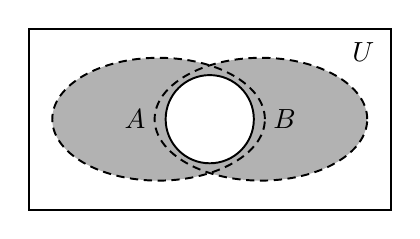
\begin{tikzpicture}[scale=1,line width=0.7pt]
\draw (0,0) rectangle (4.6,2.3);
\fill[black!30] (1.65,1.15) ellipse (1.35 and 0.78);
\fill[black!30] (2.95,1.15) ellipse (1.35 and 0.78);
\fill[white] (2.3,1.15) circle (0.56);
\draw[densely dashed] (1.65,1.15) ellipse (1.35 and 0.78);
\draw[densely dashed] (2.95,1.15) ellipse (1.35 and 0.78);
\draw (2.3,1.15) circle (0.56);
\node at (1.35,1.15) {$A$};
\node at (3.25,1.15) {$B$};
\node at (4.25,2.0) {$U$};
\end{tikzpicture}
\end{center}

\keepwithprev
A. $(-2,1)$\qquad B. $[-1,0]\cup[1,2)$\qquad C. $(-2,-1)\cup[0,1]$\qquad D. $[0,1]$

\ifanswer
\solbegin
\step{$A=\{x\mid-2<x<0\}$，$B=\{x\mid-1\leqslant x\leqslant1\}$，}
\step{所以 $A\cap B=\{x\mid-1\leqslant x<0\}$，$A\cup B=\{x\mid-2<x\leqslant1\}$，}
\step{则图中阴影部分表示的集合是 $(-2,-1)\cup[0,1]$，故选 $C$.}
\solend
\fi

\item 用反证法证明：“若 $x$、$y\in\R$ 且 $x+y>2$，则 $x$、$y$ 中至少有一个大于 $1$”时，应假设\mbox{（\quad）}% 原卷括号内已印“D”，试卷版按惯例留空

\keepwithprev
A. $x$、$y$ 中至少有一个小于 $1$\qquad B. $x$、$y$ 均小于 $1$

C. $x$、$y$ 中至少有一个小于等于 $1$\qquad D. $x$、$y$ 均小于等于 $1$

\ifanswer
\ans{$D$}
\fi

\item 若关于 $x$ 的不等式 $ax^2+bx+c>0$ 的解集是 $(-1,2)$，则不等式 $\dfrac{3ax-b}{x-3}>0$ 的解集是\mbox{（\quad）}

\keepwithprev
A. $\left(-\infty,-\dfrac13\right)\cup(3,+\infty)$\qquad B. $\left(-\dfrac13,3\right)$

C. $(-\infty,-3)\cup\left(\dfrac13,+\infty\right)$\qquad D. $\left(-3,\dfrac13\right)$

\ifanswer
\solbegin
\step{因为不等式 $ax^2+bx+c>0$ 的解集是 $(-1,2)$，}
\step{所以 $-1$、$2$ 是方程 $ax^2+bx+c=0$ 的两个根，且 $a<0$，}
\step{所以 $\begin{cases}-1+2=-\dfrac ba\\ -1\times2=\dfrac ca\end{cases}\Rightarrow\begin{cases}b=-a\\ c=-2a\end{cases}$，}
\step{所以 $\dfrac{3ax-b}{x-3}>0\Rightarrow\dfrac{3ax+a}{x-3}>0\Leftrightarrow a(3x+1)(x-3)>0$，}
\step{又 $a<0$，所以 $(3x+1)(x-3)<0$，解得 $-\dfrac13<x<3$，}
\step{所以不等式 $\dfrac{3ax-b}{x-3}>0$ 的解集为 $\left(-\dfrac13,3\right)$，故选 $B$.}
\solend
\fi

\end{enumerate}

\bigsec{三、解答题}

\begin{enumerate}
\setcounter{enumi}{16}

\item 解下列不等式组：

（1）$\begin{cases}\dfrac{5-x}{x+3}>0\\ 2x-\lvert x-1\rvert>2\end{cases}$；\qquad（2）$\begin{cases}-x^2+x+6\geqslant0\\ \dfrac{x-2}{x+1}\geqslant0\end{cases}$.

\ansspace*[12]

\ifanswer
\solbegin
\stepm{（1）}{不等式 $\dfrac{5-x}{x+3}>0$ 等价于 $(x-5)(x+3)<0$，所以 $-3<x<5$，}
\step{不等式 $2x-\lvert x-1\rvert>2$ 等价于 $2x-2>\lvert x-1\rvert$，}
\step{所以 $2-2x<x-1<2x-2$，故 $x>1$，}
\step{所以不等式组的解集为 $(1,5)$；}
\stepm{（2）}{不等式组 $\begin{cases}-x^2+x+6\geqslant0\\ \dfrac{x-2}{x+1}\geqslant0\end{cases}$ 可化为 $\begin{cases}x^2-x-6\leqslant0\\ (x-2)(x+1)\geqslant0\\ x+1\neq0\end{cases}$，}
\step{解得 $\begin{cases}-2\leqslant x\leqslant3\\ x\leqslant-1\ \text{或}\ x\geqslant2\\ x\neq-1\end{cases}$，即 $-2\leqslant x<-1$ 或 $2\leqslant x\leqslant3$，}
\step{所以不等式组的解集为 $\{x\mid-2\leqslant x<-1$ 或 $2\leqslant x\leqslant3\}$.}
\solend
\fi

\needvspace{3.2cm}
\item 已知 $A=\{x\mid x^2-2x-3\leqslant0\}$，$B=\{x\mid a-1\leqslant x\leqslant2a+1\}$，$a\in\R$.

（1）若 $A\cap B=B$，求实数 $a$ 的取值范围.

（2）若 $a>b>0$，比较 $\dfrac{a^2-b^2}{a^2+b^2}$ 与 $\dfrac{a-b}{a+b}$ 的大小.

\ansspace*[13]

\ifanswer
\solbegin
\stepm{（1）}{解不等式 $x^2-2x-3\leqslant0$，得 $-1\leqslant x\leqslant3$，}
\step{因为 $A\cap B=B$，所以 $B\subseteq A$，}
\step{当 $B=\varnothing$ 时，则 $a-1>2a+1$，解得 $a<-2$，}
\step{当 $B\neq\varnothing$ 时，要使得 $B\subseteq A$，则满足 $\begin{cases}a-1\leqslant2a+1\\ a-1\geqslant-1\\ 2a+1\leqslant3\end{cases}$，解得 $0\leqslant a\leqslant1$，}
\step{综上，实数 $a$ 的取值范围为 $(-\infty,-2)\cup[0,1]$.}
\stepm{（2）}{因为 $a>b>0$，所以 $a-b>0$，$a+b>0$，$ab>0$，}
\step{所以 $a^2-b^2=(a-b)(a+b)>0$，$a^2+b^2+2ab>a^2+b^2>0$，}
\step{$\dfrac{a^2-b^2}{a^2+b^2}>0$，$\dfrac{a-b}{a+b}>0$，}
\step{$\dfrac{\dfrac{a^2-b^2}{a^2+b^2}}{\dfrac{a-b}{a+b}}=\dfrac{(a-b)(a+b)}{a^2+b^2}\cdot\dfrac{a+b}{a-b}=\dfrac{a^2+b^2+2ab}{a^2+b^2}>1$，}
\step{所以 $\dfrac{a^2-b^2}{a^2+b^2}>\dfrac{a-b}{a+b}$.}
\solend
\fi

\item 汽车在行驶中，由于惯性作用，刹车后还要继续向前滑行一段距离才能停住，我们称这段距离为“刹车距离”. 刹车距离是分析事故的一个重要因素. 在一个限速 $40\mathrm{km}/\mathrm{h}$ 以内的弯道上，甲、乙两辆汽车相向而行，发现情况不对，同时刹车，但还是相碰了，事发后现场测得甲车的刹车距离略超过 $12\mathrm{m}$，乙车的刹车距离略超过 $10\mathrm{m}$，又知甲、乙两种车型的刹车距离 $s(\mathrm{m})$ 与车速 $x(\mathrm{km}/\mathrm{h})$ 之间有如下关系：$s_{\text{甲}}=0.1x+0.01x^2$，$s_{\text{乙}}=0.05x+0.005x^2$. 问：两车相撞的主要责任是谁？

\ansspace*[10]

\ifanswer
\solbegin
\step{由题意列出不等式组 $\begin{cases}0.1x+0.01x^2>12\\ 0.05x+0.005x^2>10\end{cases}$，解得 $\begin{cases}x<-40\ \text{或}\ x>30\\ x<-50\ \text{或}\ x>40\end{cases}$，}
\step{由于 $x>0$，从而可得 $x_{\text{甲}}>30\mathrm{km}/\mathrm{h}$，$x_{\text{乙}}>40\mathrm{km}/\mathrm{h}$.}
\step{经比较得乙车超过限速，应负主要责任.}
\solend
\fi

\item 已知关于 $x$ 的一元二次方程 $x^2+(2m-1)x+m^2-3=0$ 有实数根.

（1）若方程有两个负根，求实数 $m$ 的取值范围；

（2）当 $m=2$ 时，记方程的根为 $x_1$、$x_2$，求代数式 $\lvert x_1-x_2\rvert$ 的值.

\ansspace*[12]

\ifanswer
\solbegin
\stepm{（1）}{由方程有两个负根，得 $\begin{cases}\Delta=(2m-1)^2-4(m^2-3)\geqslant0\\ -(2m-1)<0\\ m^2-3>0\end{cases}$，}
\step{即 $\begin{cases}13-4m\geqslant0\\ 2m-1>0\\ (m-\sqrt3)(m+\sqrt3)>0\end{cases}$，解得 $\sqrt3<m\leqslant\dfrac{13}4$，}
\step{则实数 $m$ 的取值范围为 $\left\{m\left|\sqrt3<m\leqslant\dfrac{13}4\right.\right\}$.}
\stepm{（2）}{当 $m=2$ 时，方程为 $x^2+3x+1=0$，}
\step{此时 $\Delta=3^2-4=5>0$，且 $x_1+x_2=-3$，$x_1x_2=1$，}
\step{则 $\lvert x_1-x_2\rvert=\sqrt{(x_1+x_2)^2-4x_1x_2}=\sqrt{(-3)^2-4}=\sqrt5$.}
\solend
\fi

\item 已知不等式 $\lvert2x-a\rvert\leqslant b$ 的解集为 $A$，不等式 $mx^2-mx-1<0$ 的解集为 $B$.

（1）若 $a=1$，$b=2$，求 $A$.

（2）若 $A=[-1,3]$，求实数 $a$、$b$ 的取值；

（3）若 $B=\R$，求实数 $m$ 的取值范围.

\ansspace*[12]

\ifanswer
\solbegin
\stepm{（1）}{因为 $a=1$，$b=2$，所以不等式 $\lvert2x-a\rvert\leqslant b$ 等价于 $\lvert2x-1\rvert\leqslant2$，}
\step{所以 $-2\leqslant2x-1\leqslant2$，故 $-\dfrac12\leqslant x\leqslant\dfrac32$，所以 $A=\left[-\dfrac12,\dfrac32\right]$；}
\stepm{（2）}{当 $b>0$ 时，不等式 $\lvert2x-a\rvert\leqslant b$ 可化为 $-b\leqslant2x-a\leqslant b$，}
\step{所以 $\dfrac{a-b}2\leqslant x\leqslant\dfrac{a+b}2$，由 $A=[-1,3]$，得 $\dfrac{a-b}2=-1$，$\dfrac{a+b}2=3$；}
\step{当 $b=0$ 时，不等式 $\lvert2x-a\rvert\leqslant b$ 的解集为 $\left\{\dfrac a2\right\}$，不满足要求，}
\step{当 $b<0$ 时，不等式 $\lvert2x-a\rvert\leqslant b$ 的解集为 $\varnothing$，不满足要求，}
\step{所以 $a=2$，$b=4$；}
\stepm{（3）}{由已知不等式 $mx^2-mx-1<0$ 的解集为 $\R$，}
\step{得 $\begin{cases}m<0\\ m^2+4m<0\end{cases}$ 或 $m=0$，解得 $-4<m<0$ 或 $m=0$，}
\step{所以实数 $m$ 的取值范围为 $(-4,0]$.}
\solend
\fi

\end{enumerate}

\end{document}
"
% 紧凑版：xelatex "\def\iscompact{1}% 高一97_浦东中学_10月月考.tex
%   —— 高一上数学“2026-2027 年浦东中学高一上 10 月月考”（讲评版）
% 试卷版：xelatex 高一97_浦东中学_10月月考.tex
% 答案版：xelatex "\def\isanswer{1}\input{高一97_浦东中学_10月月考.tex}"
% 紧凑版：xelatex "\def\iscompact{1}\input{高一97_浦东中学_10月月考.tex}"
%
% 原始材料：微信公众号“魔都数学加油站”文章，连载“27学年高一97”；
% 原文标题“27学年高一97——2026-2027年上海市浦东中学高一上10月月考”；
% 原文链接：https://mp.weixin.qq.com/s/2uW3LikOX3B07IWw7LkF_g。
% 正文为 8 张 PNG 页（`原图/高一97_浦东中学_10月月考/01..08.png`）：04、08 为
% 2560×3620，其余为 4762×6735，按页序读取。
%
% 篇幅与题号：原卷自第 3 题起编号（第 1、2 题不在原文内）。填空题 3—12（10 题）、
% 选择题 13—16（4 题）、解答题 17—21（5 题），共 19 题。
%
% 讲评版：第 15 题无【解析】、答案“D”直接印在题干括号内，本稿试卷版按惯例留空、
% 答案版提 \ans{}；其余 18 题印【解析】，其中第 13、14、16 题的答案在解析末句
% “故选 $B$／$C$／$B$”。
%
% 副标题：原卷未印副标题。本稿按内容标作“集合与常用逻辑用语、不等式”。
%
% 插图：第 14 题题干右侧有一幅韦恩图（全集 $U$ 的矩形内两个相交椭圆 $A$、$B$，
% 阴影为两椭圆的对称差）。原图该页为 2560×3620 的低分辨率页，直接裁切会糊，
% 故按原图布局用 TikZ 重绘（三版都出）。
%
% 与原卷的排版差异：
%   ① 原卷每题下直接印【答案】/【解析】，本稿按全稿惯例将答案与解析置于答案版；
%   ② 原卷未印副标题，本稿补出；填空横线统一排 \blankline[4.4em]；
%   ③ 原卷数集记号排斜体 $R$，本稿按全稿惯例改用 $\R$；
%   ④ 第 14 题的韦恩图原为行内右侧小图，本稿改为居中单列；
%   ⑤ 解答题按惯例加 \ansspace；选择题括号排 \mbox{（\quad）}。
%
% 行数核对：逐题数 \step/\stepm 条数，合计 85 条（Q3：2；Q4：2；Q5：2；Q6：2；
% Q7：2；Q8：4；Q9：4；Q10：5；Q11：10；Q12：3；Q13：4；Q14：3；Q15：0；
% Q16：6；Q17：7；Q18：10；Q19：3；Q20：6；Q21：10）。第 15 题无解析，
% 不计入 \step 账。原卷解析的换行按语意合并，未逐行强拆。
%
\documentclass[a4paper,11pt]{article}
\usepackage{common}

\begin{document}

\examtitlest[2]{2026--2027 年浦东中学高一上 10 月月考}{集合与常用逻辑用语、不等式}

\bigsec{一、填空题}

\begin{enumerate}
\setcounter{enumi}{2}

\item “$a(a-2)<0$”是“$\dfrac2a>1$”成立的\blankline[4.4em]条件（填充分必要性）.

\ifanswer
\solbegin
\step{“不等式 $a(a-2)<0\Rightarrow0<a<2$，不等式 $\dfrac2a>1\Rightarrow\dfrac{2-a}a>0\Rightarrow0<a<2$，}
\step{两不等式解集相等，所以“$a(a-2)<0$”是“$\dfrac2a>1$”成立的充要条件.}
\solend
\fi

\item 求不等式 $\lvert5-2x\rvert\leqslant3$ 的解集\blankline[4.4em].

\ifanswer
\solbegin
\step{$\lvert5-2x\rvert\leqslant3$ 等价于 $-3\leqslant5-2x\leqslant3$，解得 $1\leqslant x\leqslant4$，}
\step{所以不等式 $\lvert5-2x\rvert\leqslant3$ 的解集为 $\{x\mid1\leqslant x\leqslant4\}$.}
\solend
\fi

\item 求不等式组 $\begin{cases}3x^2+2x-1<0\\ \dfrac1x\geqslant0\end{cases}$ 的解集\blankline[4.4em].

\ifanswer
\solbegin
\step{不等式 $3x^2+2x-1=(3x-1)(x+1)<0$，解得 $-1<x<\dfrac13$，}
\step{由不等式 $\dfrac1x\geqslant0$ 解得 $x>0$，所以不等式组的解集为 $\left(0,\dfrac13\right)$.}
\solend
\fi

\item 满足 $\{1,3\}\subseteq A\subseteq\{0,1,3,5\}$ 的所有集合 $A$ 的全部元素之和为\blankline[4.4em].

\ifanswer
\solbegin
\step{符合条件的集合 $A$ 有以下几个，$A_1=\{0,1,3\}$，$A_2=\{1,3,5\}$，$A_3=\{0,1,3,5\}$，}
\step{所以所有集合 $A$ 的全部元素之和为 $0+1+3+1+3+5+0+1+3+5=22$.}
\solend
\fi

\item 已知集合 $A=\{(x,y)\mid y=-x+1\}$，$B=\{(x,y)\mid y=x^2-1\}$，则 $A\cap B=\blankline[4.4em]$.

\ifanswer
\solbegin
\step{联立 $\begin{cases}y=-x+1\\ y=x^2-1\end{cases}$，解得 $\begin{cases}x=1\\ y=0\end{cases}$ 或 $\begin{cases}x=-2\\ y=3\end{cases}$，}
\step{故 $A\cap B=\{(1,0),(-2,3)\}$.}
\solend
\fi

\item 若 $a$、$b$ 是方程 $x^2+2x-3=0$ 的两个实数根，则 $a^2-2b=\blankline[4.4em]$.

\ifanswer
\solbegin
\step{$a$、$b$ 是方程 $x^2+2x-3=0$ 的两个实数根，}
\step{所以 $a^2+2a-3=0$，故 $a^2=3-2a$，}
\step{由韦达定理得 $a+b=-2$，所以 $b=-2-a$，}
\step{所以 $a^2-2b=3-2a-2b=3-2a+4+2a=7$.}
\solend
\fi

\item 设 $a$、$b$ 为实数，若不等式 $x^2-ax-b<0$ 的解集为 $(2,8)$，则 $bx^2-ax-1>0$ 的解集为\blankline[4.4em].

\ifanswer
\solbegin
\step{因为不等式 $x^2-ax-b<0$ 的解集为 $(2,8)$，所以 $\begin{cases}2+8=a\\ 2\times8=-b\end{cases}$，}
\step{所以 $a=10$，$b=-16$，所以 $bx^2-ax-1>0$ 可化为 $-16x^2-10x-1>0$，}
\step{所以 $16x^2+10x+1<0$，}
\step{所以所求不等式的解集为 $\left(-\dfrac12,-\dfrac18\right)$.}
\solend
\fi

\item 若集合 $A=\{x\mid x^2+3x-4=0\}$，$B=\{x\mid ax-1=0\}$，若 $A\cap B=B$，则实数 $a$ 的取值组成的集合是\blankline[4.4em].

\ifanswer
\solbegin
\step{集合 $A=\{x\mid x^2+3x-4=0\}=\{-4,1\}$，$B=\{x\mid ax-1=0\}$，}
\step{因为 $A\cap B=B$，所以 $B\subseteq A$，}
\step{当 $a=0$ 时，$B=\varnothing$，$B\subseteq A$ 成立；}
\step{当 $a\neq0$ 时，$B=\left\{\dfrac1a\right\}$，由 $B\subseteq A$，得 $\dfrac1a=-4$ 或 $\dfrac1a=1$，解得 $a=-\dfrac14$ 或 $a=1$，}
\step{所以实数 $a$ 的值为 $-\dfrac14$ 或 $0$ 或 $1$，实数 $a$ 的取值组成的集合是 $\left\{-\dfrac14,0,1\right\}$.}
\solend
\fi

\item 关于 $x$ 的不等式 $ax^2+(1-2a^2)x-2a<0$ 的解集中恰有 $3$ 个正整数解，则 $a$ 的取值范围为\blankline[4.4em].

\ifanswer
\solbegin
\step{①当 $a=0$ 时，不等式化为 $x<0$，则解集中有无数个整数，不满足题意；}
\step{当 $a\neq0$ 时，不等式 $ax^2+(1-2a^2)x-2a<0$ 的解集中恰有 $3$ 个正整数解，}
\step{即为不等式 $(ax+1)(x-2a)<0$ 的解集中恰有 $3$ 个正整数解，}
\step{②当 $a<0$ 时，不等式 $(ax+1)(x-2a)<0$ 的解集中有无数个正整数，}
\step{不满足题意，}
\step{③当 $a>0$ 时，$-\dfrac1a<0,2a>0$，所以 $-\dfrac1a<2a$，}
\step{所以不等式的解集为 $\left\{x\left|-\dfrac1a<x<2a\right.\right\}$，}
\step{由解集得 $0$ 一定属于此集合，则由不等式的解集中恰有 $3$ 个正整数，}
\step{则这 $3$ 个正整数一定为 $1$，$2$，$3$，则 $3<2a\leqslant4$，解得 $\dfrac32<a\leqslant2$，}
\step{所以 $a$ 的取值范围是 $\left\{a\left|\dfrac32<a\leqslant2\right.\right\}$.}
\solend
\fi

\item 设 $x\in\R$，$[x]$ 表示不大于 $x$ 的最大整数，如 $[\pi]=3$，$[-1.2]=-2$，$\left[\dfrac12\right]=0$，则使 $[\lvert x-1\rvert]=3$ 成立的 $x$ 的取值范围\blankline[4.4em].

\ifanswer
\solbegin
\step{由题意 $[\lvert x-1\rvert]=3$，则 $3\leqslant\lvert x-1\rvert<4$，所以 $3\leqslant x-1<4$ 或 $-4\leqslant x-1<-3$，}
\step{解得 $4\leqslant x<5$ 或 $-3<x\leqslant-2$，}
\step{所以使 $[\lvert x-1\rvert]=3$ 成立的 $x$ 的取值范围是 $(-3,-2]\cup[4,5)$.}
\solend
\fi

\end{enumerate}

\bigsec{二、选择题}

\begin{enumerate}
\setcounter{enumi}{12}

\item 若 $a\in\R$，则“$a^2>a$”是“$a>1$”的\mbox{（\quad）}

\keepwithprev
A. 充分非必要条件\qquad B. 必要非充分条件

C. 充要条件\qquad D. 既非充分又非必要条件

\ifanswer
\solbegin
\step{已知 $a^2>a$，则 $a(a-1)>0$，即 $a<0$ 或 $a>1$，}
\step{由“$a<0$ 或 $a>1$”不能推出“$a>1$”；}
\step{由“$a>1$”可以推出“$a<0$ 或 $a>1$”，即“$a>1$”可以推出“$a^2>a$”；}
\step{所以“$a^2>a$”是“$a>1$”的必要非充分条件. 故选 $B$.}
\solend
\fi

\item 已知全集 $U=\R$，集合 $A=\{x\mid x(x+2)<0\}$，$B=\{x\mid\lvert x\rvert\leqslant1\}$，则图中阴影部分表示的集合是\mbox{（\quad）}

\begin{center}
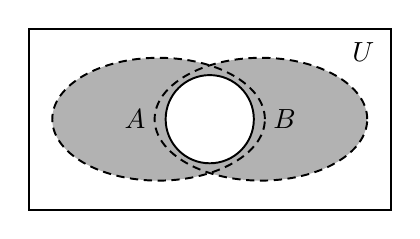
\begin{tikzpicture}[scale=1,line width=0.7pt]
\draw (0,0) rectangle (4.6,2.3);
\fill[black!30] (1.65,1.15) ellipse (1.35 and 0.78);
\fill[black!30] (2.95,1.15) ellipse (1.35 and 0.78);
\fill[white] (2.3,1.15) circle (0.56);
\draw[densely dashed] (1.65,1.15) ellipse (1.35 and 0.78);
\draw[densely dashed] (2.95,1.15) ellipse (1.35 and 0.78);
\draw (2.3,1.15) circle (0.56);
\node at (1.35,1.15) {$A$};
\node at (3.25,1.15) {$B$};
\node at (4.25,2.0) {$U$};
\end{tikzpicture}
\end{center}

\keepwithprev
A. $(-2,1)$\qquad B. $[-1,0]\cup[1,2)$\qquad C. $(-2,-1)\cup[0,1]$\qquad D. $[0,1]$

\ifanswer
\solbegin
\step{$A=\{x\mid-2<x<0\}$，$B=\{x\mid-1\leqslant x\leqslant1\}$，}
\step{所以 $A\cap B=\{x\mid-1\leqslant x<0\}$，$A\cup B=\{x\mid-2<x\leqslant1\}$，}
\step{则图中阴影部分表示的集合是 $(-2,-1)\cup[0,1]$，故选 $C$.}
\solend
\fi

\item 用反证法证明：“若 $x$、$y\in\R$ 且 $x+y>2$，则 $x$、$y$ 中至少有一个大于 $1$”时，应假设\mbox{（\quad）}% 原卷括号内已印“D”，试卷版按惯例留空

\keepwithprev
A. $x$、$y$ 中至少有一个小于 $1$\qquad B. $x$、$y$ 均小于 $1$

C. $x$、$y$ 中至少有一个小于等于 $1$\qquad D. $x$、$y$ 均小于等于 $1$

\ifanswer
\ans{$D$}
\fi

\item 若关于 $x$ 的不等式 $ax^2+bx+c>0$ 的解集是 $(-1,2)$，则不等式 $\dfrac{3ax-b}{x-3}>0$ 的解集是\mbox{（\quad）}

\keepwithprev
A. $\left(-\infty,-\dfrac13\right)\cup(3,+\infty)$\qquad B. $\left(-\dfrac13,3\right)$

C. $(-\infty,-3)\cup\left(\dfrac13,+\infty\right)$\qquad D. $\left(-3,\dfrac13\right)$

\ifanswer
\solbegin
\step{因为不等式 $ax^2+bx+c>0$ 的解集是 $(-1,2)$，}
\step{所以 $-1$、$2$ 是方程 $ax^2+bx+c=0$ 的两个根，且 $a<0$，}
\step{所以 $\begin{cases}-1+2=-\dfrac ba\\ -1\times2=\dfrac ca\end{cases}\Rightarrow\begin{cases}b=-a\\ c=-2a\end{cases}$，}
\step{所以 $\dfrac{3ax-b}{x-3}>0\Rightarrow\dfrac{3ax+a}{x-3}>0\Leftrightarrow a(3x+1)(x-3)>0$，}
\step{又 $a<0$，所以 $(3x+1)(x-3)<0$，解得 $-\dfrac13<x<3$，}
\step{所以不等式 $\dfrac{3ax-b}{x-3}>0$ 的解集为 $\left(-\dfrac13,3\right)$，故选 $B$.}
\solend
\fi

\end{enumerate}

\bigsec{三、解答题}

\begin{enumerate}
\setcounter{enumi}{16}

\item 解下列不等式组：

（1）$\begin{cases}\dfrac{5-x}{x+3}>0\\ 2x-\lvert x-1\rvert>2\end{cases}$；\qquad（2）$\begin{cases}-x^2+x+6\geqslant0\\ \dfrac{x-2}{x+1}\geqslant0\end{cases}$.

\ansspace*[12]

\ifanswer
\solbegin
\stepm{（1）}{不等式 $\dfrac{5-x}{x+3}>0$ 等价于 $(x-5)(x+3)<0$，所以 $-3<x<5$，}
\step{不等式 $2x-\lvert x-1\rvert>2$ 等价于 $2x-2>\lvert x-1\rvert$，}
\step{所以 $2-2x<x-1<2x-2$，故 $x>1$，}
\step{所以不等式组的解集为 $(1,5)$；}
\stepm{（2）}{不等式组 $\begin{cases}-x^2+x+6\geqslant0\\ \dfrac{x-2}{x+1}\geqslant0\end{cases}$ 可化为 $\begin{cases}x^2-x-6\leqslant0\\ (x-2)(x+1)\geqslant0\\ x+1\neq0\end{cases}$，}
\step{解得 $\begin{cases}-2\leqslant x\leqslant3\\ x\leqslant-1\ \text{或}\ x\geqslant2\\ x\neq-1\end{cases}$，即 $-2\leqslant x<-1$ 或 $2\leqslant x\leqslant3$，}
\step{所以不等式组的解集为 $\{x\mid-2\leqslant x<-1$ 或 $2\leqslant x\leqslant3\}$.}
\solend
\fi

\needvspace{3.2cm}
\item 已知 $A=\{x\mid x^2-2x-3\leqslant0\}$，$B=\{x\mid a-1\leqslant x\leqslant2a+1\}$，$a\in\R$.

（1）若 $A\cap B=B$，求实数 $a$ 的取值范围.

（2）若 $a>b>0$，比较 $\dfrac{a^2-b^2}{a^2+b^2}$ 与 $\dfrac{a-b}{a+b}$ 的大小.

\ansspace*[13]

\ifanswer
\solbegin
\stepm{（1）}{解不等式 $x^2-2x-3\leqslant0$，得 $-1\leqslant x\leqslant3$，}
\step{因为 $A\cap B=B$，所以 $B\subseteq A$，}
\step{当 $B=\varnothing$ 时，则 $a-1>2a+1$，解得 $a<-2$，}
\step{当 $B\neq\varnothing$ 时，要使得 $B\subseteq A$，则满足 $\begin{cases}a-1\leqslant2a+1\\ a-1\geqslant-1\\ 2a+1\leqslant3\end{cases}$，解得 $0\leqslant a\leqslant1$，}
\step{综上，实数 $a$ 的取值范围为 $(-\infty,-2)\cup[0,1]$.}
\stepm{（2）}{因为 $a>b>0$，所以 $a-b>0$，$a+b>0$，$ab>0$，}
\step{所以 $a^2-b^2=(a-b)(a+b)>0$，$a^2+b^2+2ab>a^2+b^2>0$，}
\step{$\dfrac{a^2-b^2}{a^2+b^2}>0$，$\dfrac{a-b}{a+b}>0$，}
\step{$\dfrac{\dfrac{a^2-b^2}{a^2+b^2}}{\dfrac{a-b}{a+b}}=\dfrac{(a-b)(a+b)}{a^2+b^2}\cdot\dfrac{a+b}{a-b}=\dfrac{a^2+b^2+2ab}{a^2+b^2}>1$，}
\step{所以 $\dfrac{a^2-b^2}{a^2+b^2}>\dfrac{a-b}{a+b}$.}
\solend
\fi

\item 汽车在行驶中，由于惯性作用，刹车后还要继续向前滑行一段距离才能停住，我们称这段距离为“刹车距离”. 刹车距离是分析事故的一个重要因素. 在一个限速 $40\mathrm{km}/\mathrm{h}$ 以内的弯道上，甲、乙两辆汽车相向而行，发现情况不对，同时刹车，但还是相碰了，事发后现场测得甲车的刹车距离略超过 $12\mathrm{m}$，乙车的刹车距离略超过 $10\mathrm{m}$，又知甲、乙两种车型的刹车距离 $s(\mathrm{m})$ 与车速 $x(\mathrm{km}/\mathrm{h})$ 之间有如下关系：$s_{\text{甲}}=0.1x+0.01x^2$，$s_{\text{乙}}=0.05x+0.005x^2$. 问：两车相撞的主要责任是谁？

\ansspace*[10]

\ifanswer
\solbegin
\step{由题意列出不等式组 $\begin{cases}0.1x+0.01x^2>12\\ 0.05x+0.005x^2>10\end{cases}$，解得 $\begin{cases}x<-40\ \text{或}\ x>30\\ x<-50\ \text{或}\ x>40\end{cases}$，}
\step{由于 $x>0$，从而可得 $x_{\text{甲}}>30\mathrm{km}/\mathrm{h}$，$x_{\text{乙}}>40\mathrm{km}/\mathrm{h}$.}
\step{经比较得乙车超过限速，应负主要责任.}
\solend
\fi

\item 已知关于 $x$ 的一元二次方程 $x^2+(2m-1)x+m^2-3=0$ 有实数根.

（1）若方程有两个负根，求实数 $m$ 的取值范围；

（2）当 $m=2$ 时，记方程的根为 $x_1$、$x_2$，求代数式 $\lvert x_1-x_2\rvert$ 的值.

\ansspace*[12]

\ifanswer
\solbegin
\stepm{（1）}{由方程有两个负根，得 $\begin{cases}\Delta=(2m-1)^2-4(m^2-3)\geqslant0\\ -(2m-1)<0\\ m^2-3>0\end{cases}$，}
\step{即 $\begin{cases}13-4m\geqslant0\\ 2m-1>0\\ (m-\sqrt3)(m+\sqrt3)>0\end{cases}$，解得 $\sqrt3<m\leqslant\dfrac{13}4$，}
\step{则实数 $m$ 的取值范围为 $\left\{m\left|\sqrt3<m\leqslant\dfrac{13}4\right.\right\}$.}
\stepm{（2）}{当 $m=2$ 时，方程为 $x^2+3x+1=0$，}
\step{此时 $\Delta=3^2-4=5>0$，且 $x_1+x_2=-3$，$x_1x_2=1$，}
\step{则 $\lvert x_1-x_2\rvert=\sqrt{(x_1+x_2)^2-4x_1x_2}=\sqrt{(-3)^2-4}=\sqrt5$.}
\solend
\fi

\item 已知不等式 $\lvert2x-a\rvert\leqslant b$ 的解集为 $A$，不等式 $mx^2-mx-1<0$ 的解集为 $B$.

（1）若 $a=1$，$b=2$，求 $A$.

（2）若 $A=[-1,3]$，求实数 $a$、$b$ 的取值；

（3）若 $B=\R$，求实数 $m$ 的取值范围.

\ansspace*[12]

\ifanswer
\solbegin
\stepm{（1）}{因为 $a=1$，$b=2$，所以不等式 $\lvert2x-a\rvert\leqslant b$ 等价于 $\lvert2x-1\rvert\leqslant2$，}
\step{所以 $-2\leqslant2x-1\leqslant2$，故 $-\dfrac12\leqslant x\leqslant\dfrac32$，所以 $A=\left[-\dfrac12,\dfrac32\right]$；}
\stepm{（2）}{当 $b>0$ 时，不等式 $\lvert2x-a\rvert\leqslant b$ 可化为 $-b\leqslant2x-a\leqslant b$，}
\step{所以 $\dfrac{a-b}2\leqslant x\leqslant\dfrac{a+b}2$，由 $A=[-1,3]$，得 $\dfrac{a-b}2=-1$，$\dfrac{a+b}2=3$；}
\step{当 $b=0$ 时，不等式 $\lvert2x-a\rvert\leqslant b$ 的解集为 $\left\{\dfrac a2\right\}$，不满足要求，}
\step{当 $b<0$ 时，不等式 $\lvert2x-a\rvert\leqslant b$ 的解集为 $\varnothing$，不满足要求，}
\step{所以 $a=2$，$b=4$；}
\stepm{（3）}{由已知不等式 $mx^2-mx-1<0$ 的解集为 $\R$，}
\step{得 $\begin{cases}m<0\\ m^2+4m<0\end{cases}$ 或 $m=0$，解得 $-4<m<0$ 或 $m=0$，}
\step{所以实数 $m$ 的取值范围为 $(-4,0]$.}
\solend
\fi

\end{enumerate}

\end{document}
"
%
% 原始材料：微信公众号“魔都数学加油站”文章，连载“27学年高一97”；
% 原文标题“27学年高一97——2026-2027年上海市浦东中学高一上10月月考”；
% 原文链接：https://mp.weixin.qq.com/s/2uW3LikOX3B07IWw7LkF_g。
% 正文为 8 张 PNG 页（`原图/高一97_浦东中学_10月月考/01..08.png`）：04、08 为
% 2560×3620，其余为 4762×6735，按页序读取。
%
% 篇幅与题号：原卷自第 3 题起编号（第 1、2 题不在原文内）。填空题 3—12（10 题）、
% 选择题 13—16（4 题）、解答题 17—21（5 题），共 19 题。
%
% 讲评版：第 15 题无【解析】、答案“D”直接印在题干括号内，本稿试卷版按惯例留空、
% 答案版提 \ans{}；其余 18 题印【解析】，其中第 13、14、16 题的答案在解析末句
% “故选 $B$／$C$／$B$”。
%
% 副标题：原卷未印副标题。本稿按内容标作“集合与常用逻辑用语、不等式”。
%
% 插图：第 14 题题干右侧有一幅韦恩图（全集 $U$ 的矩形内两个相交椭圆 $A$、$B$，
% 阴影为两椭圆的对称差）。原图该页为 2560×3620 的低分辨率页，直接裁切会糊，
% 故按原图布局用 TikZ 重绘（三版都出）。
%
% 与原卷的排版差异：
%   ① 原卷每题下直接印【答案】/【解析】，本稿按全稿惯例将答案与解析置于答案版；
%   ② 原卷未印副标题，本稿补出；填空横线统一排 \blankline[4.4em]；
%   ③ 原卷数集记号排斜体 $R$，本稿按全稿惯例改用 $\R$；
%   ④ 第 14 题的韦恩图原为行内右侧小图，本稿改为居中单列；
%   ⑤ 解答题按惯例加 \ansspace；选择题括号排 \mbox{（\quad）}。
%
% 行数核对：逐题数 \step/\stepm 条数，合计 85 条（Q3：2；Q4：2；Q5：2；Q6：2；
% Q7：2；Q8：4；Q9：4；Q10：5；Q11：10；Q12：3；Q13：4；Q14：3；Q15：0；
% Q16：6；Q17：7；Q18：10；Q19：3；Q20：6；Q21：10）。第 15 题无解析，
% 不计入 \step 账。原卷解析的换行按语意合并，未逐行强拆。
%
\documentclass[a4paper,11pt]{article}
\usepackage{common}

\begin{document}

\examtitlest[2]{2026--2027 年浦东中学高一上 10 月月考}{集合与常用逻辑用语、不等式}

\bigsec{一、填空题}

\begin{enumerate}
\setcounter{enumi}{2}

\item “$a(a-2)<0$”是“$\dfrac2a>1$”成立的\blankline[4.4em]条件（填充分必要性）.

\ifanswer
\solbegin
\step{“不等式 $a(a-2)<0\Rightarrow0<a<2$，不等式 $\dfrac2a>1\Rightarrow\dfrac{2-a}a>0\Rightarrow0<a<2$，}
\step{两不等式解集相等，所以“$a(a-2)<0$”是“$\dfrac2a>1$”成立的充要条件.}
\solend
\fi

\item 求不等式 $\lvert5-2x\rvert\leqslant3$ 的解集\blankline[4.4em].

\ifanswer
\solbegin
\step{$\lvert5-2x\rvert\leqslant3$ 等价于 $-3\leqslant5-2x\leqslant3$，解得 $1\leqslant x\leqslant4$，}
\step{所以不等式 $\lvert5-2x\rvert\leqslant3$ 的解集为 $\{x\mid1\leqslant x\leqslant4\}$.}
\solend
\fi

\item 求不等式组 $\begin{cases}3x^2+2x-1<0\\ \dfrac1x\geqslant0\end{cases}$ 的解集\blankline[4.4em].

\ifanswer
\solbegin
\step{不等式 $3x^2+2x-1=(3x-1)(x+1)<0$，解得 $-1<x<\dfrac13$，}
\step{由不等式 $\dfrac1x\geqslant0$ 解得 $x>0$，所以不等式组的解集为 $\left(0,\dfrac13\right)$.}
\solend
\fi

\item 满足 $\{1,3\}\subseteq A\subseteq\{0,1,3,5\}$ 的所有集合 $A$ 的全部元素之和为\blankline[4.4em].

\ifanswer
\solbegin
\step{符合条件的集合 $A$ 有以下几个，$A_1=\{0,1,3\}$，$A_2=\{1,3,5\}$，$A_3=\{0,1,3,5\}$，}
\step{所以所有集合 $A$ 的全部元素之和为 $0+1+3+1+3+5+0+1+3+5=22$.}
\solend
\fi

\item 已知集合 $A=\{(x,y)\mid y=-x+1\}$，$B=\{(x,y)\mid y=x^2-1\}$，则 $A\cap B=\blankline[4.4em]$.

\ifanswer
\solbegin
\step{联立 $\begin{cases}y=-x+1\\ y=x^2-1\end{cases}$，解得 $\begin{cases}x=1\\ y=0\end{cases}$ 或 $\begin{cases}x=-2\\ y=3\end{cases}$，}
\step{故 $A\cap B=\{(1,0),(-2,3)\}$.}
\solend
\fi

\item 若 $a$、$b$ 是方程 $x^2+2x-3=0$ 的两个实数根，则 $a^2-2b=\blankline[4.4em]$.

\ifanswer
\solbegin
\step{$a$、$b$ 是方程 $x^2+2x-3=0$ 的两个实数根，}
\step{所以 $a^2+2a-3=0$，故 $a^2=3-2a$，}
\step{由韦达定理得 $a+b=-2$，所以 $b=-2-a$，}
\step{所以 $a^2-2b=3-2a-2b=3-2a+4+2a=7$.}
\solend
\fi

\item 设 $a$、$b$ 为实数，若不等式 $x^2-ax-b<0$ 的解集为 $(2,8)$，则 $bx^2-ax-1>0$ 的解集为\blankline[4.4em].

\ifanswer
\solbegin
\step{因为不等式 $x^2-ax-b<0$ 的解集为 $(2,8)$，所以 $\begin{cases}2+8=a\\ 2\times8=-b\end{cases}$，}
\step{所以 $a=10$，$b=-16$，所以 $bx^2-ax-1>0$ 可化为 $-16x^2-10x-1>0$，}
\step{所以 $16x^2+10x+1<0$，}
\step{所以所求不等式的解集为 $\left(-\dfrac12,-\dfrac18\right)$.}
\solend
\fi

\item 若集合 $A=\{x\mid x^2+3x-4=0\}$，$B=\{x\mid ax-1=0\}$，若 $A\cap B=B$，则实数 $a$ 的取值组成的集合是\blankline[4.4em].

\ifanswer
\solbegin
\step{集合 $A=\{x\mid x^2+3x-4=0\}=\{-4,1\}$，$B=\{x\mid ax-1=0\}$，}
\step{因为 $A\cap B=B$，所以 $B\subseteq A$，}
\step{当 $a=0$ 时，$B=\varnothing$，$B\subseteq A$ 成立；}
\step{当 $a\neq0$ 时，$B=\left\{\dfrac1a\right\}$，由 $B\subseteq A$，得 $\dfrac1a=-4$ 或 $\dfrac1a=1$，解得 $a=-\dfrac14$ 或 $a=1$，}
\step{所以实数 $a$ 的值为 $-\dfrac14$ 或 $0$ 或 $1$，实数 $a$ 的取值组成的集合是 $\left\{-\dfrac14,0,1\right\}$.}
\solend
\fi

\item 关于 $x$ 的不等式 $ax^2+(1-2a^2)x-2a<0$ 的解集中恰有 $3$ 个正整数解，则 $a$ 的取值范围为\blankline[4.4em].

\ifanswer
\solbegin
\step{①当 $a=0$ 时，不等式化为 $x<0$，则解集中有无数个整数，不满足题意；}
\step{当 $a\neq0$ 时，不等式 $ax^2+(1-2a^2)x-2a<0$ 的解集中恰有 $3$ 个正整数解，}
\step{即为不等式 $(ax+1)(x-2a)<0$ 的解集中恰有 $3$ 个正整数解，}
\step{②当 $a<0$ 时，不等式 $(ax+1)(x-2a)<0$ 的解集中有无数个正整数，}
\step{不满足题意，}
\step{③当 $a>0$ 时，$-\dfrac1a<0,2a>0$，所以 $-\dfrac1a<2a$，}
\step{所以不等式的解集为 $\left\{x\left|-\dfrac1a<x<2a\right.\right\}$，}
\step{由解集得 $0$ 一定属于此集合，则由不等式的解集中恰有 $3$ 个正整数，}
\step{则这 $3$ 个正整数一定为 $1$，$2$，$3$，则 $3<2a\leqslant4$，解得 $\dfrac32<a\leqslant2$，}
\step{所以 $a$ 的取值范围是 $\left\{a\left|\dfrac32<a\leqslant2\right.\right\}$.}
\solend
\fi

\item 设 $x\in\R$，$[x]$ 表示不大于 $x$ 的最大整数，如 $[\pi]=3$，$[-1.2]=-2$，$\left[\dfrac12\right]=0$，则使 $[\lvert x-1\rvert]=3$ 成立的 $x$ 的取值范围\blankline[4.4em].

\ifanswer
\solbegin
\step{由题意 $[\lvert x-1\rvert]=3$，则 $3\leqslant\lvert x-1\rvert<4$，所以 $3\leqslant x-1<4$ 或 $-4\leqslant x-1<-3$，}
\step{解得 $4\leqslant x<5$ 或 $-3<x\leqslant-2$，}
\step{所以使 $[\lvert x-1\rvert]=3$ 成立的 $x$ 的取值范围是 $(-3,-2]\cup[4,5)$.}
\solend
\fi

\end{enumerate}

\bigsec{二、选择题}

\begin{enumerate}
\setcounter{enumi}{12}

\item 若 $a\in\R$，则“$a^2>a$”是“$a>1$”的\mbox{（\quad）}

\keepwithprev
A. 充分非必要条件\qquad B. 必要非充分条件

C. 充要条件\qquad D. 既非充分又非必要条件

\ifanswer
\solbegin
\step{已知 $a^2>a$，则 $a(a-1)>0$，即 $a<0$ 或 $a>1$，}
\step{由“$a<0$ 或 $a>1$”不能推出“$a>1$”；}
\step{由“$a>1$”可以推出“$a<0$ 或 $a>1$”，即“$a>1$”可以推出“$a^2>a$”；}
\step{所以“$a^2>a$”是“$a>1$”的必要非充分条件. 故选 $B$.}
\solend
\fi

\item 已知全集 $U=\R$，集合 $A=\{x\mid x(x+2)<0\}$，$B=\{x\mid\lvert x\rvert\leqslant1\}$，则图中阴影部分表示的集合是\mbox{（\quad）}

\begin{center}
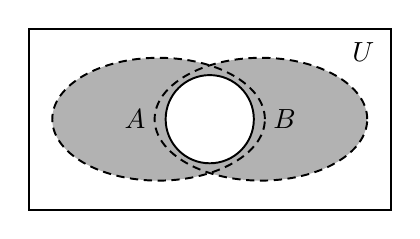
\begin{tikzpicture}[scale=1,line width=0.7pt]
\draw (0,0) rectangle (4.6,2.3);
\fill[black!30] (1.65,1.15) ellipse (1.35 and 0.78);
\fill[black!30] (2.95,1.15) ellipse (1.35 and 0.78);
\fill[white] (2.3,1.15) circle (0.56);
\draw[densely dashed] (1.65,1.15) ellipse (1.35 and 0.78);
\draw[densely dashed] (2.95,1.15) ellipse (1.35 and 0.78);
\draw (2.3,1.15) circle (0.56);
\node at (1.35,1.15) {$A$};
\node at (3.25,1.15) {$B$};
\node at (4.25,2.0) {$U$};
\end{tikzpicture}
\end{center}

\keepwithprev
A. $(-2,1)$\qquad B. $[-1,0]\cup[1,2)$\qquad C. $(-2,-1)\cup[0,1]$\qquad D. $[0,1]$

\ifanswer
\solbegin
\step{$A=\{x\mid-2<x<0\}$，$B=\{x\mid-1\leqslant x\leqslant1\}$，}
\step{所以 $A\cap B=\{x\mid-1\leqslant x<0\}$，$A\cup B=\{x\mid-2<x\leqslant1\}$，}
\step{则图中阴影部分表示的集合是 $(-2,-1)\cup[0,1]$，故选 $C$.}
\solend
\fi

\item 用反证法证明：“若 $x$、$y\in\R$ 且 $x+y>2$，则 $x$、$y$ 中至少有一个大于 $1$”时，应假设\mbox{（\quad）}% 原卷括号内已印“D”，试卷版按惯例留空

\keepwithprev
A. $x$、$y$ 中至少有一个小于 $1$\qquad B. $x$、$y$ 均小于 $1$

C. $x$、$y$ 中至少有一个小于等于 $1$\qquad D. $x$、$y$ 均小于等于 $1$

\ifanswer
\ans{$D$}
\fi

\item 若关于 $x$ 的不等式 $ax^2+bx+c>0$ 的解集是 $(-1,2)$，则不等式 $\dfrac{3ax-b}{x-3}>0$ 的解集是\mbox{（\quad）}

\keepwithprev
A. $\left(-\infty,-\dfrac13\right)\cup(3,+\infty)$\qquad B. $\left(-\dfrac13,3\right)$

C. $(-\infty,-3)\cup\left(\dfrac13,+\infty\right)$\qquad D. $\left(-3,\dfrac13\right)$

\ifanswer
\solbegin
\step{因为不等式 $ax^2+bx+c>0$ 的解集是 $(-1,2)$，}
\step{所以 $-1$、$2$ 是方程 $ax^2+bx+c=0$ 的两个根，且 $a<0$，}
\step{所以 $\begin{cases}-1+2=-\dfrac ba\\ -1\times2=\dfrac ca\end{cases}\Rightarrow\begin{cases}b=-a\\ c=-2a\end{cases}$，}
\step{所以 $\dfrac{3ax-b}{x-3}>0\Rightarrow\dfrac{3ax+a}{x-3}>0\Leftrightarrow a(3x+1)(x-3)>0$，}
\step{又 $a<0$，所以 $(3x+1)(x-3)<0$，解得 $-\dfrac13<x<3$，}
\step{所以不等式 $\dfrac{3ax-b}{x-3}>0$ 的解集为 $\left(-\dfrac13,3\right)$，故选 $B$.}
\solend
\fi

\end{enumerate}

\bigsec{三、解答题}

\begin{enumerate}
\setcounter{enumi}{16}

\item 解下列不等式组：

（1）$\begin{cases}\dfrac{5-x}{x+3}>0\\ 2x-\lvert x-1\rvert>2\end{cases}$；\qquad（2）$\begin{cases}-x^2+x+6\geqslant0\\ \dfrac{x-2}{x+1}\geqslant0\end{cases}$.

\ansspace*[12]

\ifanswer
\solbegin
\stepm{（1）}{不等式 $\dfrac{5-x}{x+3}>0$ 等价于 $(x-5)(x+3)<0$，所以 $-3<x<5$，}
\step{不等式 $2x-\lvert x-1\rvert>2$ 等价于 $2x-2>\lvert x-1\rvert$，}
\step{所以 $2-2x<x-1<2x-2$，故 $x>1$，}
\step{所以不等式组的解集为 $(1,5)$；}
\stepm{（2）}{不等式组 $\begin{cases}-x^2+x+6\geqslant0\\ \dfrac{x-2}{x+1}\geqslant0\end{cases}$ 可化为 $\begin{cases}x^2-x-6\leqslant0\\ (x-2)(x+1)\geqslant0\\ x+1\neq0\end{cases}$，}
\step{解得 $\begin{cases}-2\leqslant x\leqslant3\\ x\leqslant-1\ \text{或}\ x\geqslant2\\ x\neq-1\end{cases}$，即 $-2\leqslant x<-1$ 或 $2\leqslant x\leqslant3$，}
\step{所以不等式组的解集为 $\{x\mid-2\leqslant x<-1$ 或 $2\leqslant x\leqslant3\}$.}
\solend
\fi

\needvspace{3.2cm}
\item 已知 $A=\{x\mid x^2-2x-3\leqslant0\}$，$B=\{x\mid a-1\leqslant x\leqslant2a+1\}$，$a\in\R$.

（1）若 $A\cap B=B$，求实数 $a$ 的取值范围.

（2）若 $a>b>0$，比较 $\dfrac{a^2-b^2}{a^2+b^2}$ 与 $\dfrac{a-b}{a+b}$ 的大小.

\ansspace*[13]

\ifanswer
\solbegin
\stepm{（1）}{解不等式 $x^2-2x-3\leqslant0$，得 $-1\leqslant x\leqslant3$，}
\step{因为 $A\cap B=B$，所以 $B\subseteq A$，}
\step{当 $B=\varnothing$ 时，则 $a-1>2a+1$，解得 $a<-2$，}
\step{当 $B\neq\varnothing$ 时，要使得 $B\subseteq A$，则满足 $\begin{cases}a-1\leqslant2a+1\\ a-1\geqslant-1\\ 2a+1\leqslant3\end{cases}$，解得 $0\leqslant a\leqslant1$，}
\step{综上，实数 $a$ 的取值范围为 $(-\infty,-2)\cup[0,1]$.}
\stepm{（2）}{因为 $a>b>0$，所以 $a-b>0$，$a+b>0$，$ab>0$，}
\step{所以 $a^2-b^2=(a-b)(a+b)>0$，$a^2+b^2+2ab>a^2+b^2>0$，}
\step{$\dfrac{a^2-b^2}{a^2+b^2}>0$，$\dfrac{a-b}{a+b}>0$，}
\step{$\dfrac{\dfrac{a^2-b^2}{a^2+b^2}}{\dfrac{a-b}{a+b}}=\dfrac{(a-b)(a+b)}{a^2+b^2}\cdot\dfrac{a+b}{a-b}=\dfrac{a^2+b^2+2ab}{a^2+b^2}>1$，}
\step{所以 $\dfrac{a^2-b^2}{a^2+b^2}>\dfrac{a-b}{a+b}$.}
\solend
\fi

\item 汽车在行驶中，由于惯性作用，刹车后还要继续向前滑行一段距离才能停住，我们称这段距离为“刹车距离”. 刹车距离是分析事故的一个重要因素. 在一个限速 $40\mathrm{km}/\mathrm{h}$ 以内的弯道上，甲、乙两辆汽车相向而行，发现情况不对，同时刹车，但还是相碰了，事发后现场测得甲车的刹车距离略超过 $12\mathrm{m}$，乙车的刹车距离略超过 $10\mathrm{m}$，又知甲、乙两种车型的刹车距离 $s(\mathrm{m})$ 与车速 $x(\mathrm{km}/\mathrm{h})$ 之间有如下关系：$s_{\text{甲}}=0.1x+0.01x^2$，$s_{\text{乙}}=0.05x+0.005x^2$. 问：两车相撞的主要责任是谁？

\ansspace*[10]

\ifanswer
\solbegin
\step{由题意列出不等式组 $\begin{cases}0.1x+0.01x^2>12\\ 0.05x+0.005x^2>10\end{cases}$，解得 $\begin{cases}x<-40\ \text{或}\ x>30\\ x<-50\ \text{或}\ x>40\end{cases}$，}
\step{由于 $x>0$，从而可得 $x_{\text{甲}}>30\mathrm{km}/\mathrm{h}$，$x_{\text{乙}}>40\mathrm{km}/\mathrm{h}$.}
\step{经比较得乙车超过限速，应负主要责任.}
\solend
\fi

\item 已知关于 $x$ 的一元二次方程 $x^2+(2m-1)x+m^2-3=0$ 有实数根.

（1）若方程有两个负根，求实数 $m$ 的取值范围；

（2）当 $m=2$ 时，记方程的根为 $x_1$、$x_2$，求代数式 $\lvert x_1-x_2\rvert$ 的值.

\ansspace*[12]

\ifanswer
\solbegin
\stepm{（1）}{由方程有两个负根，得 $\begin{cases}\Delta=(2m-1)^2-4(m^2-3)\geqslant0\\ -(2m-1)<0\\ m^2-3>0\end{cases}$，}
\step{即 $\begin{cases}13-4m\geqslant0\\ 2m-1>0\\ (m-\sqrt3)(m+\sqrt3)>0\end{cases}$，解得 $\sqrt3<m\leqslant\dfrac{13}4$，}
\step{则实数 $m$ 的取值范围为 $\left\{m\left|\sqrt3<m\leqslant\dfrac{13}4\right.\right\}$.}
\stepm{（2）}{当 $m=2$ 时，方程为 $x^2+3x+1=0$，}
\step{此时 $\Delta=3^2-4=5>0$，且 $x_1+x_2=-3$，$x_1x_2=1$，}
\step{则 $\lvert x_1-x_2\rvert=\sqrt{(x_1+x_2)^2-4x_1x_2}=\sqrt{(-3)^2-4}=\sqrt5$.}
\solend
\fi

\item 已知不等式 $\lvert2x-a\rvert\leqslant b$ 的解集为 $A$，不等式 $mx^2-mx-1<0$ 的解集为 $B$.

（1）若 $a=1$，$b=2$，求 $A$.

（2）若 $A=[-1,3]$，求实数 $a$、$b$ 的取值；

（3）若 $B=\R$，求实数 $m$ 的取值范围.

\ansspace*[12]

\ifanswer
\solbegin
\stepm{（1）}{因为 $a=1$，$b=2$，所以不等式 $\lvert2x-a\rvert\leqslant b$ 等价于 $\lvert2x-1\rvert\leqslant2$，}
\step{所以 $-2\leqslant2x-1\leqslant2$，故 $-\dfrac12\leqslant x\leqslant\dfrac32$，所以 $A=\left[-\dfrac12,\dfrac32\right]$；}
\stepm{（2）}{当 $b>0$ 时，不等式 $\lvert2x-a\rvert\leqslant b$ 可化为 $-b\leqslant2x-a\leqslant b$，}
\step{所以 $\dfrac{a-b}2\leqslant x\leqslant\dfrac{a+b}2$，由 $A=[-1,3]$，得 $\dfrac{a-b}2=-1$，$\dfrac{a+b}2=3$；}
\step{当 $b=0$ 时，不等式 $\lvert2x-a\rvert\leqslant b$ 的解集为 $\left\{\dfrac a2\right\}$，不满足要求，}
\step{当 $b<0$ 时，不等式 $\lvert2x-a\rvert\leqslant b$ 的解集为 $\varnothing$，不满足要求，}
\step{所以 $a=2$，$b=4$；}
\stepm{（3）}{由已知不等式 $mx^2-mx-1<0$ 的解集为 $\R$，}
\step{得 $\begin{cases}m<0\\ m^2+4m<0\end{cases}$ 或 $m=0$，解得 $-4<m<0$ 或 $m=0$，}
\step{所以实数 $m$ 的取值范围为 $(-4,0]$.}
\solend
\fi

\end{enumerate}

\end{document}
"
% 紧凑版：xelatex "\def\iscompact{1}% 高一97_浦东中学_10月月考.tex
%   —— 高一上数学“2026-2027 年浦东中学高一上 10 月月考”（讲评版）
% 试卷版：xelatex 高一97_浦东中学_10月月考.tex
% 答案版：xelatex "\def\isanswer{1}% 高一97_浦东中学_10月月考.tex
%   —— 高一上数学“2026-2027 年浦东中学高一上 10 月月考”（讲评版）
% 试卷版：xelatex 高一97_浦东中学_10月月考.tex
% 答案版：xelatex "\def\isanswer{1}\input{高一97_浦东中学_10月月考.tex}"
% 紧凑版：xelatex "\def\iscompact{1}\input{高一97_浦东中学_10月月考.tex}"
%
% 原始材料：微信公众号“魔都数学加油站”文章，连载“27学年高一97”；
% 原文标题“27学年高一97——2026-2027年上海市浦东中学高一上10月月考”；
% 原文链接：https://mp.weixin.qq.com/s/2uW3LikOX3B07IWw7LkF_g。
% 正文为 8 张 PNG 页（`原图/高一97_浦东中学_10月月考/01..08.png`）：04、08 为
% 2560×3620，其余为 4762×6735，按页序读取。
%
% 篇幅与题号：原卷自第 3 题起编号（第 1、2 题不在原文内）。填空题 3—12（10 题）、
% 选择题 13—16（4 题）、解答题 17—21（5 题），共 19 题。
%
% 讲评版：第 15 题无【解析】、答案“D”直接印在题干括号内，本稿试卷版按惯例留空、
% 答案版提 \ans{}；其余 18 题印【解析】，其中第 13、14、16 题的答案在解析末句
% “故选 $B$／$C$／$B$”。
%
% 副标题：原卷未印副标题。本稿按内容标作“集合与常用逻辑用语、不等式”。
%
% 插图：第 14 题题干右侧有一幅韦恩图（全集 $U$ 的矩形内两个相交椭圆 $A$、$B$，
% 阴影为两椭圆的对称差）。原图该页为 2560×3620 的低分辨率页，直接裁切会糊，
% 故按原图布局用 TikZ 重绘（三版都出）。
%
% 与原卷的排版差异：
%   ① 原卷每题下直接印【答案】/【解析】，本稿按全稿惯例将答案与解析置于答案版；
%   ② 原卷未印副标题，本稿补出；填空横线统一排 \blankline[4.4em]；
%   ③ 原卷数集记号排斜体 $R$，本稿按全稿惯例改用 $\R$；
%   ④ 第 14 题的韦恩图原为行内右侧小图，本稿改为居中单列；
%   ⑤ 解答题按惯例加 \ansspace；选择题括号排 \mbox{（\quad）}。
%
% 行数核对：逐题数 \step/\stepm 条数，合计 85 条（Q3：2；Q4：2；Q5：2；Q6：2；
% Q7：2；Q8：4；Q9：4；Q10：5；Q11：10；Q12：3；Q13：4；Q14：3；Q15：0；
% Q16：6；Q17：7；Q18：10；Q19：3；Q20：6；Q21：10）。第 15 题无解析，
% 不计入 \step 账。原卷解析的换行按语意合并，未逐行强拆。
%
\documentclass[a4paper,11pt]{article}
\usepackage{common}

\begin{document}

\examtitlest[2]{2026--2027 年浦东中学高一上 10 月月考}{集合与常用逻辑用语、不等式}

\bigsec{一、填空题}

\begin{enumerate}
\setcounter{enumi}{2}

\item “$a(a-2)<0$”是“$\dfrac2a>1$”成立的\blankline[4.4em]条件（填充分必要性）.

\ifanswer
\solbegin
\step{“不等式 $a(a-2)<0\Rightarrow0<a<2$，不等式 $\dfrac2a>1\Rightarrow\dfrac{2-a}a>0\Rightarrow0<a<2$，}
\step{两不等式解集相等，所以“$a(a-2)<0$”是“$\dfrac2a>1$”成立的充要条件.}
\solend
\fi

\item 求不等式 $\lvert5-2x\rvert\leqslant3$ 的解集\blankline[4.4em].

\ifanswer
\solbegin
\step{$\lvert5-2x\rvert\leqslant3$ 等价于 $-3\leqslant5-2x\leqslant3$，解得 $1\leqslant x\leqslant4$，}
\step{所以不等式 $\lvert5-2x\rvert\leqslant3$ 的解集为 $\{x\mid1\leqslant x\leqslant4\}$.}
\solend
\fi

\item 求不等式组 $\begin{cases}3x^2+2x-1<0\\ \dfrac1x\geqslant0\end{cases}$ 的解集\blankline[4.4em].

\ifanswer
\solbegin
\step{不等式 $3x^2+2x-1=(3x-1)(x+1)<0$，解得 $-1<x<\dfrac13$，}
\step{由不等式 $\dfrac1x\geqslant0$ 解得 $x>0$，所以不等式组的解集为 $\left(0,\dfrac13\right)$.}
\solend
\fi

\item 满足 $\{1,3\}\subseteq A\subseteq\{0,1,3,5\}$ 的所有集合 $A$ 的全部元素之和为\blankline[4.4em].

\ifanswer
\solbegin
\step{符合条件的集合 $A$ 有以下几个，$A_1=\{0,1,3\}$，$A_2=\{1,3,5\}$，$A_3=\{0,1,3,5\}$，}
\step{所以所有集合 $A$ 的全部元素之和为 $0+1+3+1+3+5+0+1+3+5=22$.}
\solend
\fi

\item 已知集合 $A=\{(x,y)\mid y=-x+1\}$，$B=\{(x,y)\mid y=x^2-1\}$，则 $A\cap B=\blankline[4.4em]$.

\ifanswer
\solbegin
\step{联立 $\begin{cases}y=-x+1\\ y=x^2-1\end{cases}$，解得 $\begin{cases}x=1\\ y=0\end{cases}$ 或 $\begin{cases}x=-2\\ y=3\end{cases}$，}
\step{故 $A\cap B=\{(1,0),(-2,3)\}$.}
\solend
\fi

\item 若 $a$、$b$ 是方程 $x^2+2x-3=0$ 的两个实数根，则 $a^2-2b=\blankline[4.4em]$.

\ifanswer
\solbegin
\step{$a$、$b$ 是方程 $x^2+2x-3=0$ 的两个实数根，}
\step{所以 $a^2+2a-3=0$，故 $a^2=3-2a$，}
\step{由韦达定理得 $a+b=-2$，所以 $b=-2-a$，}
\step{所以 $a^2-2b=3-2a-2b=3-2a+4+2a=7$.}
\solend
\fi

\item 设 $a$、$b$ 为实数，若不等式 $x^2-ax-b<0$ 的解集为 $(2,8)$，则 $bx^2-ax-1>0$ 的解集为\blankline[4.4em].

\ifanswer
\solbegin
\step{因为不等式 $x^2-ax-b<0$ 的解集为 $(2,8)$，所以 $\begin{cases}2+8=a\\ 2\times8=-b\end{cases}$，}
\step{所以 $a=10$，$b=-16$，所以 $bx^2-ax-1>0$ 可化为 $-16x^2-10x-1>0$，}
\step{所以 $16x^2+10x+1<0$，}
\step{所以所求不等式的解集为 $\left(-\dfrac12,-\dfrac18\right)$.}
\solend
\fi

\item 若集合 $A=\{x\mid x^2+3x-4=0\}$，$B=\{x\mid ax-1=0\}$，若 $A\cap B=B$，则实数 $a$ 的取值组成的集合是\blankline[4.4em].

\ifanswer
\solbegin
\step{集合 $A=\{x\mid x^2+3x-4=0\}=\{-4,1\}$，$B=\{x\mid ax-1=0\}$，}
\step{因为 $A\cap B=B$，所以 $B\subseteq A$，}
\step{当 $a=0$ 时，$B=\varnothing$，$B\subseteq A$ 成立；}
\step{当 $a\neq0$ 时，$B=\left\{\dfrac1a\right\}$，由 $B\subseteq A$，得 $\dfrac1a=-4$ 或 $\dfrac1a=1$，解得 $a=-\dfrac14$ 或 $a=1$，}
\step{所以实数 $a$ 的值为 $-\dfrac14$ 或 $0$ 或 $1$，实数 $a$ 的取值组成的集合是 $\left\{-\dfrac14,0,1\right\}$.}
\solend
\fi

\item 关于 $x$ 的不等式 $ax^2+(1-2a^2)x-2a<0$ 的解集中恰有 $3$ 个正整数解，则 $a$ 的取值范围为\blankline[4.4em].

\ifanswer
\solbegin
\step{①当 $a=0$ 时，不等式化为 $x<0$，则解集中有无数个整数，不满足题意；}
\step{当 $a\neq0$ 时，不等式 $ax^2+(1-2a^2)x-2a<0$ 的解集中恰有 $3$ 个正整数解，}
\step{即为不等式 $(ax+1)(x-2a)<0$ 的解集中恰有 $3$ 个正整数解，}
\step{②当 $a<0$ 时，不等式 $(ax+1)(x-2a)<0$ 的解集中有无数个正整数，}
\step{不满足题意，}
\step{③当 $a>0$ 时，$-\dfrac1a<0,2a>0$，所以 $-\dfrac1a<2a$，}
\step{所以不等式的解集为 $\left\{x\left|-\dfrac1a<x<2a\right.\right\}$，}
\step{由解集得 $0$ 一定属于此集合，则由不等式的解集中恰有 $3$ 个正整数，}
\step{则这 $3$ 个正整数一定为 $1$，$2$，$3$，则 $3<2a\leqslant4$，解得 $\dfrac32<a\leqslant2$，}
\step{所以 $a$ 的取值范围是 $\left\{a\left|\dfrac32<a\leqslant2\right.\right\}$.}
\solend
\fi

\item 设 $x\in\R$，$[x]$ 表示不大于 $x$ 的最大整数，如 $[\pi]=3$，$[-1.2]=-2$，$\left[\dfrac12\right]=0$，则使 $[\lvert x-1\rvert]=3$ 成立的 $x$ 的取值范围\blankline[4.4em].

\ifanswer
\solbegin
\step{由题意 $[\lvert x-1\rvert]=3$，则 $3\leqslant\lvert x-1\rvert<4$，所以 $3\leqslant x-1<4$ 或 $-4\leqslant x-1<-3$，}
\step{解得 $4\leqslant x<5$ 或 $-3<x\leqslant-2$，}
\step{所以使 $[\lvert x-1\rvert]=3$ 成立的 $x$ 的取值范围是 $(-3,-2]\cup[4,5)$.}
\solend
\fi

\end{enumerate}

\bigsec{二、选择题}

\begin{enumerate}
\setcounter{enumi}{12}

\item 若 $a\in\R$，则“$a^2>a$”是“$a>1$”的\mbox{（\quad）}

\keepwithprev
A. 充分非必要条件\qquad B. 必要非充分条件

C. 充要条件\qquad D. 既非充分又非必要条件

\ifanswer
\solbegin
\step{已知 $a^2>a$，则 $a(a-1)>0$，即 $a<0$ 或 $a>1$，}
\step{由“$a<0$ 或 $a>1$”不能推出“$a>1$”；}
\step{由“$a>1$”可以推出“$a<0$ 或 $a>1$”，即“$a>1$”可以推出“$a^2>a$”；}
\step{所以“$a^2>a$”是“$a>1$”的必要非充分条件. 故选 $B$.}
\solend
\fi

\item 已知全集 $U=\R$，集合 $A=\{x\mid x(x+2)<0\}$，$B=\{x\mid\lvert x\rvert\leqslant1\}$，则图中阴影部分表示的集合是\mbox{（\quad）}

\begin{center}
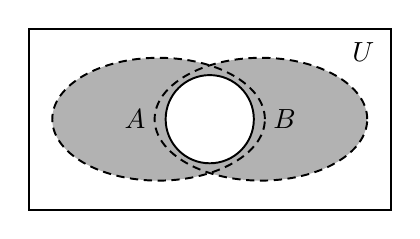
\begin{tikzpicture}[scale=1,line width=0.7pt]
\draw (0,0) rectangle (4.6,2.3);
\fill[black!30] (1.65,1.15) ellipse (1.35 and 0.78);
\fill[black!30] (2.95,1.15) ellipse (1.35 and 0.78);
\fill[white] (2.3,1.15) circle (0.56);
\draw[densely dashed] (1.65,1.15) ellipse (1.35 and 0.78);
\draw[densely dashed] (2.95,1.15) ellipse (1.35 and 0.78);
\draw (2.3,1.15) circle (0.56);
\node at (1.35,1.15) {$A$};
\node at (3.25,1.15) {$B$};
\node at (4.25,2.0) {$U$};
\end{tikzpicture}
\end{center}

\keepwithprev
A. $(-2,1)$\qquad B. $[-1,0]\cup[1,2)$\qquad C. $(-2,-1)\cup[0,1]$\qquad D. $[0,1]$

\ifanswer
\solbegin
\step{$A=\{x\mid-2<x<0\}$，$B=\{x\mid-1\leqslant x\leqslant1\}$，}
\step{所以 $A\cap B=\{x\mid-1\leqslant x<0\}$，$A\cup B=\{x\mid-2<x\leqslant1\}$，}
\step{则图中阴影部分表示的集合是 $(-2,-1)\cup[0,1]$，故选 $C$.}
\solend
\fi

\item 用反证法证明：“若 $x$、$y\in\R$ 且 $x+y>2$，则 $x$、$y$ 中至少有一个大于 $1$”时，应假设\mbox{（\quad）}% 原卷括号内已印“D”，试卷版按惯例留空

\keepwithprev
A. $x$、$y$ 中至少有一个小于 $1$\qquad B. $x$、$y$ 均小于 $1$

C. $x$、$y$ 中至少有一个小于等于 $1$\qquad D. $x$、$y$ 均小于等于 $1$

\ifanswer
\ans{$D$}
\fi

\item 若关于 $x$ 的不等式 $ax^2+bx+c>0$ 的解集是 $(-1,2)$，则不等式 $\dfrac{3ax-b}{x-3}>0$ 的解集是\mbox{（\quad）}

\keepwithprev
A. $\left(-\infty,-\dfrac13\right)\cup(3,+\infty)$\qquad B. $\left(-\dfrac13,3\right)$

C. $(-\infty,-3)\cup\left(\dfrac13,+\infty\right)$\qquad D. $\left(-3,\dfrac13\right)$

\ifanswer
\solbegin
\step{因为不等式 $ax^2+bx+c>0$ 的解集是 $(-1,2)$，}
\step{所以 $-1$、$2$ 是方程 $ax^2+bx+c=0$ 的两个根，且 $a<0$，}
\step{所以 $\begin{cases}-1+2=-\dfrac ba\\ -1\times2=\dfrac ca\end{cases}\Rightarrow\begin{cases}b=-a\\ c=-2a\end{cases}$，}
\step{所以 $\dfrac{3ax-b}{x-3}>0\Rightarrow\dfrac{3ax+a}{x-3}>0\Leftrightarrow a(3x+1)(x-3)>0$，}
\step{又 $a<0$，所以 $(3x+1)(x-3)<0$，解得 $-\dfrac13<x<3$，}
\step{所以不等式 $\dfrac{3ax-b}{x-3}>0$ 的解集为 $\left(-\dfrac13,3\right)$，故选 $B$.}
\solend
\fi

\end{enumerate}

\bigsec{三、解答题}

\begin{enumerate}
\setcounter{enumi}{16}

\item 解下列不等式组：

（1）$\begin{cases}\dfrac{5-x}{x+3}>0\\ 2x-\lvert x-1\rvert>2\end{cases}$；\qquad（2）$\begin{cases}-x^2+x+6\geqslant0\\ \dfrac{x-2}{x+1}\geqslant0\end{cases}$.

\ansspace*[12]

\ifanswer
\solbegin
\stepm{（1）}{不等式 $\dfrac{5-x}{x+3}>0$ 等价于 $(x-5)(x+3)<0$，所以 $-3<x<5$，}
\step{不等式 $2x-\lvert x-1\rvert>2$ 等价于 $2x-2>\lvert x-1\rvert$，}
\step{所以 $2-2x<x-1<2x-2$，故 $x>1$，}
\step{所以不等式组的解集为 $(1,5)$；}
\stepm{（2）}{不等式组 $\begin{cases}-x^2+x+6\geqslant0\\ \dfrac{x-2}{x+1}\geqslant0\end{cases}$ 可化为 $\begin{cases}x^2-x-6\leqslant0\\ (x-2)(x+1)\geqslant0\\ x+1\neq0\end{cases}$，}
\step{解得 $\begin{cases}-2\leqslant x\leqslant3\\ x\leqslant-1\ \text{或}\ x\geqslant2\\ x\neq-1\end{cases}$，即 $-2\leqslant x<-1$ 或 $2\leqslant x\leqslant3$，}
\step{所以不等式组的解集为 $\{x\mid-2\leqslant x<-1$ 或 $2\leqslant x\leqslant3\}$.}
\solend
\fi

\needvspace{3.2cm}
\item 已知 $A=\{x\mid x^2-2x-3\leqslant0\}$，$B=\{x\mid a-1\leqslant x\leqslant2a+1\}$，$a\in\R$.

（1）若 $A\cap B=B$，求实数 $a$ 的取值范围.

（2）若 $a>b>0$，比较 $\dfrac{a^2-b^2}{a^2+b^2}$ 与 $\dfrac{a-b}{a+b}$ 的大小.

\ansspace*[13]

\ifanswer
\solbegin
\stepm{（1）}{解不等式 $x^2-2x-3\leqslant0$，得 $-1\leqslant x\leqslant3$，}
\step{因为 $A\cap B=B$，所以 $B\subseteq A$，}
\step{当 $B=\varnothing$ 时，则 $a-1>2a+1$，解得 $a<-2$，}
\step{当 $B\neq\varnothing$ 时，要使得 $B\subseteq A$，则满足 $\begin{cases}a-1\leqslant2a+1\\ a-1\geqslant-1\\ 2a+1\leqslant3\end{cases}$，解得 $0\leqslant a\leqslant1$，}
\step{综上，实数 $a$ 的取值范围为 $(-\infty,-2)\cup[0,1]$.}
\stepm{（2）}{因为 $a>b>0$，所以 $a-b>0$，$a+b>0$，$ab>0$，}
\step{所以 $a^2-b^2=(a-b)(a+b)>0$，$a^2+b^2+2ab>a^2+b^2>0$，}
\step{$\dfrac{a^2-b^2}{a^2+b^2}>0$，$\dfrac{a-b}{a+b}>0$，}
\step{$\dfrac{\dfrac{a^2-b^2}{a^2+b^2}}{\dfrac{a-b}{a+b}}=\dfrac{(a-b)(a+b)}{a^2+b^2}\cdot\dfrac{a+b}{a-b}=\dfrac{a^2+b^2+2ab}{a^2+b^2}>1$，}
\step{所以 $\dfrac{a^2-b^2}{a^2+b^2}>\dfrac{a-b}{a+b}$.}
\solend
\fi

\item 汽车在行驶中，由于惯性作用，刹车后还要继续向前滑行一段距离才能停住，我们称这段距离为“刹车距离”. 刹车距离是分析事故的一个重要因素. 在一个限速 $40\mathrm{km}/\mathrm{h}$ 以内的弯道上，甲、乙两辆汽车相向而行，发现情况不对，同时刹车，但还是相碰了，事发后现场测得甲车的刹车距离略超过 $12\mathrm{m}$，乙车的刹车距离略超过 $10\mathrm{m}$，又知甲、乙两种车型的刹车距离 $s(\mathrm{m})$ 与车速 $x(\mathrm{km}/\mathrm{h})$ 之间有如下关系：$s_{\text{甲}}=0.1x+0.01x^2$，$s_{\text{乙}}=0.05x+0.005x^2$. 问：两车相撞的主要责任是谁？

\ansspace*[10]

\ifanswer
\solbegin
\step{由题意列出不等式组 $\begin{cases}0.1x+0.01x^2>12\\ 0.05x+0.005x^2>10\end{cases}$，解得 $\begin{cases}x<-40\ \text{或}\ x>30\\ x<-50\ \text{或}\ x>40\end{cases}$，}
\step{由于 $x>0$，从而可得 $x_{\text{甲}}>30\mathrm{km}/\mathrm{h}$，$x_{\text{乙}}>40\mathrm{km}/\mathrm{h}$.}
\step{经比较得乙车超过限速，应负主要责任.}
\solend
\fi

\item 已知关于 $x$ 的一元二次方程 $x^2+(2m-1)x+m^2-3=0$ 有实数根.

（1）若方程有两个负根，求实数 $m$ 的取值范围；

（2）当 $m=2$ 时，记方程的根为 $x_1$、$x_2$，求代数式 $\lvert x_1-x_2\rvert$ 的值.

\ansspace*[12]

\ifanswer
\solbegin
\stepm{（1）}{由方程有两个负根，得 $\begin{cases}\Delta=(2m-1)^2-4(m^2-3)\geqslant0\\ -(2m-1)<0\\ m^2-3>0\end{cases}$，}
\step{即 $\begin{cases}13-4m\geqslant0\\ 2m-1>0\\ (m-\sqrt3)(m+\sqrt3)>0\end{cases}$，解得 $\sqrt3<m\leqslant\dfrac{13}4$，}
\step{则实数 $m$ 的取值范围为 $\left\{m\left|\sqrt3<m\leqslant\dfrac{13}4\right.\right\}$.}
\stepm{（2）}{当 $m=2$ 时，方程为 $x^2+3x+1=0$，}
\step{此时 $\Delta=3^2-4=5>0$，且 $x_1+x_2=-3$，$x_1x_2=1$，}
\step{则 $\lvert x_1-x_2\rvert=\sqrt{(x_1+x_2)^2-4x_1x_2}=\sqrt{(-3)^2-4}=\sqrt5$.}
\solend
\fi

\item 已知不等式 $\lvert2x-a\rvert\leqslant b$ 的解集为 $A$，不等式 $mx^2-mx-1<0$ 的解集为 $B$.

（1）若 $a=1$，$b=2$，求 $A$.

（2）若 $A=[-1,3]$，求实数 $a$、$b$ 的取值；

（3）若 $B=\R$，求实数 $m$ 的取值范围.

\ansspace*[12]

\ifanswer
\solbegin
\stepm{（1）}{因为 $a=1$，$b=2$，所以不等式 $\lvert2x-a\rvert\leqslant b$ 等价于 $\lvert2x-1\rvert\leqslant2$，}
\step{所以 $-2\leqslant2x-1\leqslant2$，故 $-\dfrac12\leqslant x\leqslant\dfrac32$，所以 $A=\left[-\dfrac12,\dfrac32\right]$；}
\stepm{（2）}{当 $b>0$ 时，不等式 $\lvert2x-a\rvert\leqslant b$ 可化为 $-b\leqslant2x-a\leqslant b$，}
\step{所以 $\dfrac{a-b}2\leqslant x\leqslant\dfrac{a+b}2$，由 $A=[-1,3]$，得 $\dfrac{a-b}2=-1$，$\dfrac{a+b}2=3$；}
\step{当 $b=0$ 时，不等式 $\lvert2x-a\rvert\leqslant b$ 的解集为 $\left\{\dfrac a2\right\}$，不满足要求，}
\step{当 $b<0$ 时，不等式 $\lvert2x-a\rvert\leqslant b$ 的解集为 $\varnothing$，不满足要求，}
\step{所以 $a=2$，$b=4$；}
\stepm{（3）}{由已知不等式 $mx^2-mx-1<0$ 的解集为 $\R$，}
\step{得 $\begin{cases}m<0\\ m^2+4m<0\end{cases}$ 或 $m=0$，解得 $-4<m<0$ 或 $m=0$，}
\step{所以实数 $m$ 的取值范围为 $(-4,0]$.}
\solend
\fi

\end{enumerate}

\end{document}
"
% 紧凑版：xelatex "\def\iscompact{1}% 高一97_浦东中学_10月月考.tex
%   —— 高一上数学“2026-2027 年浦东中学高一上 10 月月考”（讲评版）
% 试卷版：xelatex 高一97_浦东中学_10月月考.tex
% 答案版：xelatex "\def\isanswer{1}\input{高一97_浦东中学_10月月考.tex}"
% 紧凑版：xelatex "\def\iscompact{1}\input{高一97_浦东中学_10月月考.tex}"
%
% 原始材料：微信公众号“魔都数学加油站”文章，连载“27学年高一97”；
% 原文标题“27学年高一97——2026-2027年上海市浦东中学高一上10月月考”；
% 原文链接：https://mp.weixin.qq.com/s/2uW3LikOX3B07IWw7LkF_g。
% 正文为 8 张 PNG 页（`原图/高一97_浦东中学_10月月考/01..08.png`）：04、08 为
% 2560×3620，其余为 4762×6735，按页序读取。
%
% 篇幅与题号：原卷自第 3 题起编号（第 1、2 题不在原文内）。填空题 3—12（10 题）、
% 选择题 13—16（4 题）、解答题 17—21（5 题），共 19 题。
%
% 讲评版：第 15 题无【解析】、答案“D”直接印在题干括号内，本稿试卷版按惯例留空、
% 答案版提 \ans{}；其余 18 题印【解析】，其中第 13、14、16 题的答案在解析末句
% “故选 $B$／$C$／$B$”。
%
% 副标题：原卷未印副标题。本稿按内容标作“集合与常用逻辑用语、不等式”。
%
% 插图：第 14 题题干右侧有一幅韦恩图（全集 $U$ 的矩形内两个相交椭圆 $A$、$B$，
% 阴影为两椭圆的对称差）。原图该页为 2560×3620 的低分辨率页，直接裁切会糊，
% 故按原图布局用 TikZ 重绘（三版都出）。
%
% 与原卷的排版差异：
%   ① 原卷每题下直接印【答案】/【解析】，本稿按全稿惯例将答案与解析置于答案版；
%   ② 原卷未印副标题，本稿补出；填空横线统一排 \blankline[4.4em]；
%   ③ 原卷数集记号排斜体 $R$，本稿按全稿惯例改用 $\R$；
%   ④ 第 14 题的韦恩图原为行内右侧小图，本稿改为居中单列；
%   ⑤ 解答题按惯例加 \ansspace；选择题括号排 \mbox{（\quad）}。
%
% 行数核对：逐题数 \step/\stepm 条数，合计 85 条（Q3：2；Q4：2；Q5：2；Q6：2；
% Q7：2；Q8：4；Q9：4；Q10：5；Q11：10；Q12：3；Q13：4；Q14：3；Q15：0；
% Q16：6；Q17：7；Q18：10；Q19：3；Q20：6；Q21：10）。第 15 题无解析，
% 不计入 \step 账。原卷解析的换行按语意合并，未逐行强拆。
%
\documentclass[a4paper,11pt]{article}
\usepackage{common}

\begin{document}

\examtitlest[2]{2026--2027 年浦东中学高一上 10 月月考}{集合与常用逻辑用语、不等式}

\bigsec{一、填空题}

\begin{enumerate}
\setcounter{enumi}{2}

\item “$a(a-2)<0$”是“$\dfrac2a>1$”成立的\blankline[4.4em]条件（填充分必要性）.

\ifanswer
\solbegin
\step{“不等式 $a(a-2)<0\Rightarrow0<a<2$，不等式 $\dfrac2a>1\Rightarrow\dfrac{2-a}a>0\Rightarrow0<a<2$，}
\step{两不等式解集相等，所以“$a(a-2)<0$”是“$\dfrac2a>1$”成立的充要条件.}
\solend
\fi

\item 求不等式 $\lvert5-2x\rvert\leqslant3$ 的解集\blankline[4.4em].

\ifanswer
\solbegin
\step{$\lvert5-2x\rvert\leqslant3$ 等价于 $-3\leqslant5-2x\leqslant3$，解得 $1\leqslant x\leqslant4$，}
\step{所以不等式 $\lvert5-2x\rvert\leqslant3$ 的解集为 $\{x\mid1\leqslant x\leqslant4\}$.}
\solend
\fi

\item 求不等式组 $\begin{cases}3x^2+2x-1<0\\ \dfrac1x\geqslant0\end{cases}$ 的解集\blankline[4.4em].

\ifanswer
\solbegin
\step{不等式 $3x^2+2x-1=(3x-1)(x+1)<0$，解得 $-1<x<\dfrac13$，}
\step{由不等式 $\dfrac1x\geqslant0$ 解得 $x>0$，所以不等式组的解集为 $\left(0,\dfrac13\right)$.}
\solend
\fi

\item 满足 $\{1,3\}\subseteq A\subseteq\{0,1,3,5\}$ 的所有集合 $A$ 的全部元素之和为\blankline[4.4em].

\ifanswer
\solbegin
\step{符合条件的集合 $A$ 有以下几个，$A_1=\{0,1,3\}$，$A_2=\{1,3,5\}$，$A_3=\{0,1,3,5\}$，}
\step{所以所有集合 $A$ 的全部元素之和为 $0+1+3+1+3+5+0+1+3+5=22$.}
\solend
\fi

\item 已知集合 $A=\{(x,y)\mid y=-x+1\}$，$B=\{(x,y)\mid y=x^2-1\}$，则 $A\cap B=\blankline[4.4em]$.

\ifanswer
\solbegin
\step{联立 $\begin{cases}y=-x+1\\ y=x^2-1\end{cases}$，解得 $\begin{cases}x=1\\ y=0\end{cases}$ 或 $\begin{cases}x=-2\\ y=3\end{cases}$，}
\step{故 $A\cap B=\{(1,0),(-2,3)\}$.}
\solend
\fi

\item 若 $a$、$b$ 是方程 $x^2+2x-3=0$ 的两个实数根，则 $a^2-2b=\blankline[4.4em]$.

\ifanswer
\solbegin
\step{$a$、$b$ 是方程 $x^2+2x-3=0$ 的两个实数根，}
\step{所以 $a^2+2a-3=0$，故 $a^2=3-2a$，}
\step{由韦达定理得 $a+b=-2$，所以 $b=-2-a$，}
\step{所以 $a^2-2b=3-2a-2b=3-2a+4+2a=7$.}
\solend
\fi

\item 设 $a$、$b$ 为实数，若不等式 $x^2-ax-b<0$ 的解集为 $(2,8)$，则 $bx^2-ax-1>0$ 的解集为\blankline[4.4em].

\ifanswer
\solbegin
\step{因为不等式 $x^2-ax-b<0$ 的解集为 $(2,8)$，所以 $\begin{cases}2+8=a\\ 2\times8=-b\end{cases}$，}
\step{所以 $a=10$，$b=-16$，所以 $bx^2-ax-1>0$ 可化为 $-16x^2-10x-1>0$，}
\step{所以 $16x^2+10x+1<0$，}
\step{所以所求不等式的解集为 $\left(-\dfrac12,-\dfrac18\right)$.}
\solend
\fi

\item 若集合 $A=\{x\mid x^2+3x-4=0\}$，$B=\{x\mid ax-1=0\}$，若 $A\cap B=B$，则实数 $a$ 的取值组成的集合是\blankline[4.4em].

\ifanswer
\solbegin
\step{集合 $A=\{x\mid x^2+3x-4=0\}=\{-4,1\}$，$B=\{x\mid ax-1=0\}$，}
\step{因为 $A\cap B=B$，所以 $B\subseteq A$，}
\step{当 $a=0$ 时，$B=\varnothing$，$B\subseteq A$ 成立；}
\step{当 $a\neq0$ 时，$B=\left\{\dfrac1a\right\}$，由 $B\subseteq A$，得 $\dfrac1a=-4$ 或 $\dfrac1a=1$，解得 $a=-\dfrac14$ 或 $a=1$，}
\step{所以实数 $a$ 的值为 $-\dfrac14$ 或 $0$ 或 $1$，实数 $a$ 的取值组成的集合是 $\left\{-\dfrac14,0,1\right\}$.}
\solend
\fi

\item 关于 $x$ 的不等式 $ax^2+(1-2a^2)x-2a<0$ 的解集中恰有 $3$ 个正整数解，则 $a$ 的取值范围为\blankline[4.4em].

\ifanswer
\solbegin
\step{①当 $a=0$ 时，不等式化为 $x<0$，则解集中有无数个整数，不满足题意；}
\step{当 $a\neq0$ 时，不等式 $ax^2+(1-2a^2)x-2a<0$ 的解集中恰有 $3$ 个正整数解，}
\step{即为不等式 $(ax+1)(x-2a)<0$ 的解集中恰有 $3$ 个正整数解，}
\step{②当 $a<0$ 时，不等式 $(ax+1)(x-2a)<0$ 的解集中有无数个正整数，}
\step{不满足题意，}
\step{③当 $a>0$ 时，$-\dfrac1a<0,2a>0$，所以 $-\dfrac1a<2a$，}
\step{所以不等式的解集为 $\left\{x\left|-\dfrac1a<x<2a\right.\right\}$，}
\step{由解集得 $0$ 一定属于此集合，则由不等式的解集中恰有 $3$ 个正整数，}
\step{则这 $3$ 个正整数一定为 $1$，$2$，$3$，则 $3<2a\leqslant4$，解得 $\dfrac32<a\leqslant2$，}
\step{所以 $a$ 的取值范围是 $\left\{a\left|\dfrac32<a\leqslant2\right.\right\}$.}
\solend
\fi

\item 设 $x\in\R$，$[x]$ 表示不大于 $x$ 的最大整数，如 $[\pi]=3$，$[-1.2]=-2$，$\left[\dfrac12\right]=0$，则使 $[\lvert x-1\rvert]=3$ 成立的 $x$ 的取值范围\blankline[4.4em].

\ifanswer
\solbegin
\step{由题意 $[\lvert x-1\rvert]=3$，则 $3\leqslant\lvert x-1\rvert<4$，所以 $3\leqslant x-1<4$ 或 $-4\leqslant x-1<-3$，}
\step{解得 $4\leqslant x<5$ 或 $-3<x\leqslant-2$，}
\step{所以使 $[\lvert x-1\rvert]=3$ 成立的 $x$ 的取值范围是 $(-3,-2]\cup[4,5)$.}
\solend
\fi

\end{enumerate}

\bigsec{二、选择题}

\begin{enumerate}
\setcounter{enumi}{12}

\item 若 $a\in\R$，则“$a^2>a$”是“$a>1$”的\mbox{（\quad）}

\keepwithprev
A. 充分非必要条件\qquad B. 必要非充分条件

C. 充要条件\qquad D. 既非充分又非必要条件

\ifanswer
\solbegin
\step{已知 $a^2>a$，则 $a(a-1)>0$，即 $a<0$ 或 $a>1$，}
\step{由“$a<0$ 或 $a>1$”不能推出“$a>1$”；}
\step{由“$a>1$”可以推出“$a<0$ 或 $a>1$”，即“$a>1$”可以推出“$a^2>a$”；}
\step{所以“$a^2>a$”是“$a>1$”的必要非充分条件. 故选 $B$.}
\solend
\fi

\item 已知全集 $U=\R$，集合 $A=\{x\mid x(x+2)<0\}$，$B=\{x\mid\lvert x\rvert\leqslant1\}$，则图中阴影部分表示的集合是\mbox{（\quad）}

\begin{center}
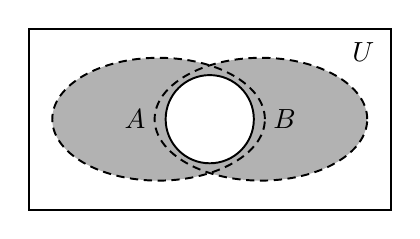
\begin{tikzpicture}[scale=1,line width=0.7pt]
\draw (0,0) rectangle (4.6,2.3);
\fill[black!30] (1.65,1.15) ellipse (1.35 and 0.78);
\fill[black!30] (2.95,1.15) ellipse (1.35 and 0.78);
\fill[white] (2.3,1.15) circle (0.56);
\draw[densely dashed] (1.65,1.15) ellipse (1.35 and 0.78);
\draw[densely dashed] (2.95,1.15) ellipse (1.35 and 0.78);
\draw (2.3,1.15) circle (0.56);
\node at (1.35,1.15) {$A$};
\node at (3.25,1.15) {$B$};
\node at (4.25,2.0) {$U$};
\end{tikzpicture}
\end{center}

\keepwithprev
A. $(-2,1)$\qquad B. $[-1,0]\cup[1,2)$\qquad C. $(-2,-1)\cup[0,1]$\qquad D. $[0,1]$

\ifanswer
\solbegin
\step{$A=\{x\mid-2<x<0\}$，$B=\{x\mid-1\leqslant x\leqslant1\}$，}
\step{所以 $A\cap B=\{x\mid-1\leqslant x<0\}$，$A\cup B=\{x\mid-2<x\leqslant1\}$，}
\step{则图中阴影部分表示的集合是 $(-2,-1)\cup[0,1]$，故选 $C$.}
\solend
\fi

\item 用反证法证明：“若 $x$、$y\in\R$ 且 $x+y>2$，则 $x$、$y$ 中至少有一个大于 $1$”时，应假设\mbox{（\quad）}% 原卷括号内已印“D”，试卷版按惯例留空

\keepwithprev
A. $x$、$y$ 中至少有一个小于 $1$\qquad B. $x$、$y$ 均小于 $1$

C. $x$、$y$ 中至少有一个小于等于 $1$\qquad D. $x$、$y$ 均小于等于 $1$

\ifanswer
\ans{$D$}
\fi

\item 若关于 $x$ 的不等式 $ax^2+bx+c>0$ 的解集是 $(-1,2)$，则不等式 $\dfrac{3ax-b}{x-3}>0$ 的解集是\mbox{（\quad）}

\keepwithprev
A. $\left(-\infty,-\dfrac13\right)\cup(3,+\infty)$\qquad B. $\left(-\dfrac13,3\right)$

C. $(-\infty,-3)\cup\left(\dfrac13,+\infty\right)$\qquad D. $\left(-3,\dfrac13\right)$

\ifanswer
\solbegin
\step{因为不等式 $ax^2+bx+c>0$ 的解集是 $(-1,2)$，}
\step{所以 $-1$、$2$ 是方程 $ax^2+bx+c=0$ 的两个根，且 $a<0$，}
\step{所以 $\begin{cases}-1+2=-\dfrac ba\\ -1\times2=\dfrac ca\end{cases}\Rightarrow\begin{cases}b=-a\\ c=-2a\end{cases}$，}
\step{所以 $\dfrac{3ax-b}{x-3}>0\Rightarrow\dfrac{3ax+a}{x-3}>0\Leftrightarrow a(3x+1)(x-3)>0$，}
\step{又 $a<0$，所以 $(3x+1)(x-3)<0$，解得 $-\dfrac13<x<3$，}
\step{所以不等式 $\dfrac{3ax-b}{x-3}>0$ 的解集为 $\left(-\dfrac13,3\right)$，故选 $B$.}
\solend
\fi

\end{enumerate}

\bigsec{三、解答题}

\begin{enumerate}
\setcounter{enumi}{16}

\item 解下列不等式组：

（1）$\begin{cases}\dfrac{5-x}{x+3}>0\\ 2x-\lvert x-1\rvert>2\end{cases}$；\qquad（2）$\begin{cases}-x^2+x+6\geqslant0\\ \dfrac{x-2}{x+1}\geqslant0\end{cases}$.

\ansspace*[12]

\ifanswer
\solbegin
\stepm{（1）}{不等式 $\dfrac{5-x}{x+3}>0$ 等价于 $(x-5)(x+3)<0$，所以 $-3<x<5$，}
\step{不等式 $2x-\lvert x-1\rvert>2$ 等价于 $2x-2>\lvert x-1\rvert$，}
\step{所以 $2-2x<x-1<2x-2$，故 $x>1$，}
\step{所以不等式组的解集为 $(1,5)$；}
\stepm{（2）}{不等式组 $\begin{cases}-x^2+x+6\geqslant0\\ \dfrac{x-2}{x+1}\geqslant0\end{cases}$ 可化为 $\begin{cases}x^2-x-6\leqslant0\\ (x-2)(x+1)\geqslant0\\ x+1\neq0\end{cases}$，}
\step{解得 $\begin{cases}-2\leqslant x\leqslant3\\ x\leqslant-1\ \text{或}\ x\geqslant2\\ x\neq-1\end{cases}$，即 $-2\leqslant x<-1$ 或 $2\leqslant x\leqslant3$，}
\step{所以不等式组的解集为 $\{x\mid-2\leqslant x<-1$ 或 $2\leqslant x\leqslant3\}$.}
\solend
\fi

\needvspace{3.2cm}
\item 已知 $A=\{x\mid x^2-2x-3\leqslant0\}$，$B=\{x\mid a-1\leqslant x\leqslant2a+1\}$，$a\in\R$.

（1）若 $A\cap B=B$，求实数 $a$ 的取值范围.

（2）若 $a>b>0$，比较 $\dfrac{a^2-b^2}{a^2+b^2}$ 与 $\dfrac{a-b}{a+b}$ 的大小.

\ansspace*[13]

\ifanswer
\solbegin
\stepm{（1）}{解不等式 $x^2-2x-3\leqslant0$，得 $-1\leqslant x\leqslant3$，}
\step{因为 $A\cap B=B$，所以 $B\subseteq A$，}
\step{当 $B=\varnothing$ 时，则 $a-1>2a+1$，解得 $a<-2$，}
\step{当 $B\neq\varnothing$ 时，要使得 $B\subseteq A$，则满足 $\begin{cases}a-1\leqslant2a+1\\ a-1\geqslant-1\\ 2a+1\leqslant3\end{cases}$，解得 $0\leqslant a\leqslant1$，}
\step{综上，实数 $a$ 的取值范围为 $(-\infty,-2)\cup[0,1]$.}
\stepm{（2）}{因为 $a>b>0$，所以 $a-b>0$，$a+b>0$，$ab>0$，}
\step{所以 $a^2-b^2=(a-b)(a+b)>0$，$a^2+b^2+2ab>a^2+b^2>0$，}
\step{$\dfrac{a^2-b^2}{a^2+b^2}>0$，$\dfrac{a-b}{a+b}>0$，}
\step{$\dfrac{\dfrac{a^2-b^2}{a^2+b^2}}{\dfrac{a-b}{a+b}}=\dfrac{(a-b)(a+b)}{a^2+b^2}\cdot\dfrac{a+b}{a-b}=\dfrac{a^2+b^2+2ab}{a^2+b^2}>1$，}
\step{所以 $\dfrac{a^2-b^2}{a^2+b^2}>\dfrac{a-b}{a+b}$.}
\solend
\fi

\item 汽车在行驶中，由于惯性作用，刹车后还要继续向前滑行一段距离才能停住，我们称这段距离为“刹车距离”. 刹车距离是分析事故的一个重要因素. 在一个限速 $40\mathrm{km}/\mathrm{h}$ 以内的弯道上，甲、乙两辆汽车相向而行，发现情况不对，同时刹车，但还是相碰了，事发后现场测得甲车的刹车距离略超过 $12\mathrm{m}$，乙车的刹车距离略超过 $10\mathrm{m}$，又知甲、乙两种车型的刹车距离 $s(\mathrm{m})$ 与车速 $x(\mathrm{km}/\mathrm{h})$ 之间有如下关系：$s_{\text{甲}}=0.1x+0.01x^2$，$s_{\text{乙}}=0.05x+0.005x^2$. 问：两车相撞的主要责任是谁？

\ansspace*[10]

\ifanswer
\solbegin
\step{由题意列出不等式组 $\begin{cases}0.1x+0.01x^2>12\\ 0.05x+0.005x^2>10\end{cases}$，解得 $\begin{cases}x<-40\ \text{或}\ x>30\\ x<-50\ \text{或}\ x>40\end{cases}$，}
\step{由于 $x>0$，从而可得 $x_{\text{甲}}>30\mathrm{km}/\mathrm{h}$，$x_{\text{乙}}>40\mathrm{km}/\mathrm{h}$.}
\step{经比较得乙车超过限速，应负主要责任.}
\solend
\fi

\item 已知关于 $x$ 的一元二次方程 $x^2+(2m-1)x+m^2-3=0$ 有实数根.

（1）若方程有两个负根，求实数 $m$ 的取值范围；

（2）当 $m=2$ 时，记方程的根为 $x_1$、$x_2$，求代数式 $\lvert x_1-x_2\rvert$ 的值.

\ansspace*[12]

\ifanswer
\solbegin
\stepm{（1）}{由方程有两个负根，得 $\begin{cases}\Delta=(2m-1)^2-4(m^2-3)\geqslant0\\ -(2m-1)<0\\ m^2-3>0\end{cases}$，}
\step{即 $\begin{cases}13-4m\geqslant0\\ 2m-1>0\\ (m-\sqrt3)(m+\sqrt3)>0\end{cases}$，解得 $\sqrt3<m\leqslant\dfrac{13}4$，}
\step{则实数 $m$ 的取值范围为 $\left\{m\left|\sqrt3<m\leqslant\dfrac{13}4\right.\right\}$.}
\stepm{（2）}{当 $m=2$ 时，方程为 $x^2+3x+1=0$，}
\step{此时 $\Delta=3^2-4=5>0$，且 $x_1+x_2=-3$，$x_1x_2=1$，}
\step{则 $\lvert x_1-x_2\rvert=\sqrt{(x_1+x_2)^2-4x_1x_2}=\sqrt{(-3)^2-4}=\sqrt5$.}
\solend
\fi

\item 已知不等式 $\lvert2x-a\rvert\leqslant b$ 的解集为 $A$，不等式 $mx^2-mx-1<0$ 的解集为 $B$.

（1）若 $a=1$，$b=2$，求 $A$.

（2）若 $A=[-1,3]$，求实数 $a$、$b$ 的取值；

（3）若 $B=\R$，求实数 $m$ 的取值范围.

\ansspace*[12]

\ifanswer
\solbegin
\stepm{（1）}{因为 $a=1$，$b=2$，所以不等式 $\lvert2x-a\rvert\leqslant b$ 等价于 $\lvert2x-1\rvert\leqslant2$，}
\step{所以 $-2\leqslant2x-1\leqslant2$，故 $-\dfrac12\leqslant x\leqslant\dfrac32$，所以 $A=\left[-\dfrac12,\dfrac32\right]$；}
\stepm{（2）}{当 $b>0$ 时，不等式 $\lvert2x-a\rvert\leqslant b$ 可化为 $-b\leqslant2x-a\leqslant b$，}
\step{所以 $\dfrac{a-b}2\leqslant x\leqslant\dfrac{a+b}2$，由 $A=[-1,3]$，得 $\dfrac{a-b}2=-1$，$\dfrac{a+b}2=3$；}
\step{当 $b=0$ 时，不等式 $\lvert2x-a\rvert\leqslant b$ 的解集为 $\left\{\dfrac a2\right\}$，不满足要求，}
\step{当 $b<0$ 时，不等式 $\lvert2x-a\rvert\leqslant b$ 的解集为 $\varnothing$，不满足要求，}
\step{所以 $a=2$，$b=4$；}
\stepm{（3）}{由已知不等式 $mx^2-mx-1<0$ 的解集为 $\R$，}
\step{得 $\begin{cases}m<0\\ m^2+4m<0\end{cases}$ 或 $m=0$，解得 $-4<m<0$ 或 $m=0$，}
\step{所以实数 $m$ 的取值范围为 $(-4,0]$.}
\solend
\fi

\end{enumerate}

\end{document}
"
%
% 原始材料：微信公众号“魔都数学加油站”文章，连载“27学年高一97”；
% 原文标题“27学年高一97——2026-2027年上海市浦东中学高一上10月月考”；
% 原文链接：https://mp.weixin.qq.com/s/2uW3LikOX3B07IWw7LkF_g。
% 正文为 8 张 PNG 页（`原图/高一97_浦东中学_10月月考/01..08.png`）：04、08 为
% 2560×3620，其余为 4762×6735，按页序读取。
%
% 篇幅与题号：原卷自第 3 题起编号（第 1、2 题不在原文内）。填空题 3—12（10 题）、
% 选择题 13—16（4 题）、解答题 17—21（5 题），共 19 题。
%
% 讲评版：第 15 题无【解析】、答案“D”直接印在题干括号内，本稿试卷版按惯例留空、
% 答案版提 \ans{}；其余 18 题印【解析】，其中第 13、14、16 题的答案在解析末句
% “故选 $B$／$C$／$B$”。
%
% 副标题：原卷未印副标题。本稿按内容标作“集合与常用逻辑用语、不等式”。
%
% 插图：第 14 题题干右侧有一幅韦恩图（全集 $U$ 的矩形内两个相交椭圆 $A$、$B$，
% 阴影为两椭圆的对称差）。原图该页为 2560×3620 的低分辨率页，直接裁切会糊，
% 故按原图布局用 TikZ 重绘（三版都出）。
%
% 与原卷的排版差异：
%   ① 原卷每题下直接印【答案】/【解析】，本稿按全稿惯例将答案与解析置于答案版；
%   ② 原卷未印副标题，本稿补出；填空横线统一排 \blankline[4.4em]；
%   ③ 原卷数集记号排斜体 $R$，本稿按全稿惯例改用 $\R$；
%   ④ 第 14 题的韦恩图原为行内右侧小图，本稿改为居中单列；
%   ⑤ 解答题按惯例加 \ansspace；选择题括号排 \mbox{（\quad）}。
%
% 行数核对：逐题数 \step/\stepm 条数，合计 85 条（Q3：2；Q4：2；Q5：2；Q6：2；
% Q7：2；Q8：4；Q9：4；Q10：5；Q11：10；Q12：3；Q13：4；Q14：3；Q15：0；
% Q16：6；Q17：7；Q18：10；Q19：3；Q20：6；Q21：10）。第 15 题无解析，
% 不计入 \step 账。原卷解析的换行按语意合并，未逐行强拆。
%
\documentclass[a4paper,11pt]{article}
\usepackage{common}

\begin{document}

\examtitlest[2]{2026--2027 年浦东中学高一上 10 月月考}{集合与常用逻辑用语、不等式}

\bigsec{一、填空题}

\begin{enumerate}
\setcounter{enumi}{2}

\item “$a(a-2)<0$”是“$\dfrac2a>1$”成立的\blankline[4.4em]条件（填充分必要性）.

\ifanswer
\solbegin
\step{“不等式 $a(a-2)<0\Rightarrow0<a<2$，不等式 $\dfrac2a>1\Rightarrow\dfrac{2-a}a>0\Rightarrow0<a<2$，}
\step{两不等式解集相等，所以“$a(a-2)<0$”是“$\dfrac2a>1$”成立的充要条件.}
\solend
\fi

\item 求不等式 $\lvert5-2x\rvert\leqslant3$ 的解集\blankline[4.4em].

\ifanswer
\solbegin
\step{$\lvert5-2x\rvert\leqslant3$ 等价于 $-3\leqslant5-2x\leqslant3$，解得 $1\leqslant x\leqslant4$，}
\step{所以不等式 $\lvert5-2x\rvert\leqslant3$ 的解集为 $\{x\mid1\leqslant x\leqslant4\}$.}
\solend
\fi

\item 求不等式组 $\begin{cases}3x^2+2x-1<0\\ \dfrac1x\geqslant0\end{cases}$ 的解集\blankline[4.4em].

\ifanswer
\solbegin
\step{不等式 $3x^2+2x-1=(3x-1)(x+1)<0$，解得 $-1<x<\dfrac13$，}
\step{由不等式 $\dfrac1x\geqslant0$ 解得 $x>0$，所以不等式组的解集为 $\left(0,\dfrac13\right)$.}
\solend
\fi

\item 满足 $\{1,3\}\subseteq A\subseteq\{0,1,3,5\}$ 的所有集合 $A$ 的全部元素之和为\blankline[4.4em].

\ifanswer
\solbegin
\step{符合条件的集合 $A$ 有以下几个，$A_1=\{0,1,3\}$，$A_2=\{1,3,5\}$，$A_3=\{0,1,3,5\}$，}
\step{所以所有集合 $A$ 的全部元素之和为 $0+1+3+1+3+5+0+1+3+5=22$.}
\solend
\fi

\item 已知集合 $A=\{(x,y)\mid y=-x+1\}$，$B=\{(x,y)\mid y=x^2-1\}$，则 $A\cap B=\blankline[4.4em]$.

\ifanswer
\solbegin
\step{联立 $\begin{cases}y=-x+1\\ y=x^2-1\end{cases}$，解得 $\begin{cases}x=1\\ y=0\end{cases}$ 或 $\begin{cases}x=-2\\ y=3\end{cases}$，}
\step{故 $A\cap B=\{(1,0),(-2,3)\}$.}
\solend
\fi

\item 若 $a$、$b$ 是方程 $x^2+2x-3=0$ 的两个实数根，则 $a^2-2b=\blankline[4.4em]$.

\ifanswer
\solbegin
\step{$a$、$b$ 是方程 $x^2+2x-3=0$ 的两个实数根，}
\step{所以 $a^2+2a-3=0$，故 $a^2=3-2a$，}
\step{由韦达定理得 $a+b=-2$，所以 $b=-2-a$，}
\step{所以 $a^2-2b=3-2a-2b=3-2a+4+2a=7$.}
\solend
\fi

\item 设 $a$、$b$ 为实数，若不等式 $x^2-ax-b<0$ 的解集为 $(2,8)$，则 $bx^2-ax-1>0$ 的解集为\blankline[4.4em].

\ifanswer
\solbegin
\step{因为不等式 $x^2-ax-b<0$ 的解集为 $(2,8)$，所以 $\begin{cases}2+8=a\\ 2\times8=-b\end{cases}$，}
\step{所以 $a=10$，$b=-16$，所以 $bx^2-ax-1>0$ 可化为 $-16x^2-10x-1>0$，}
\step{所以 $16x^2+10x+1<0$，}
\step{所以所求不等式的解集为 $\left(-\dfrac12,-\dfrac18\right)$.}
\solend
\fi

\item 若集合 $A=\{x\mid x^2+3x-4=0\}$，$B=\{x\mid ax-1=0\}$，若 $A\cap B=B$，则实数 $a$ 的取值组成的集合是\blankline[4.4em].

\ifanswer
\solbegin
\step{集合 $A=\{x\mid x^2+3x-4=0\}=\{-4,1\}$，$B=\{x\mid ax-1=0\}$，}
\step{因为 $A\cap B=B$，所以 $B\subseteq A$，}
\step{当 $a=0$ 时，$B=\varnothing$，$B\subseteq A$ 成立；}
\step{当 $a\neq0$ 时，$B=\left\{\dfrac1a\right\}$，由 $B\subseteq A$，得 $\dfrac1a=-4$ 或 $\dfrac1a=1$，解得 $a=-\dfrac14$ 或 $a=1$，}
\step{所以实数 $a$ 的值为 $-\dfrac14$ 或 $0$ 或 $1$，实数 $a$ 的取值组成的集合是 $\left\{-\dfrac14,0,1\right\}$.}
\solend
\fi

\item 关于 $x$ 的不等式 $ax^2+(1-2a^2)x-2a<0$ 的解集中恰有 $3$ 个正整数解，则 $a$ 的取值范围为\blankline[4.4em].

\ifanswer
\solbegin
\step{①当 $a=0$ 时，不等式化为 $x<0$，则解集中有无数个整数，不满足题意；}
\step{当 $a\neq0$ 时，不等式 $ax^2+(1-2a^2)x-2a<0$ 的解集中恰有 $3$ 个正整数解，}
\step{即为不等式 $(ax+1)(x-2a)<0$ 的解集中恰有 $3$ 个正整数解，}
\step{②当 $a<0$ 时，不等式 $(ax+1)(x-2a)<0$ 的解集中有无数个正整数，}
\step{不满足题意，}
\step{③当 $a>0$ 时，$-\dfrac1a<0,2a>0$，所以 $-\dfrac1a<2a$，}
\step{所以不等式的解集为 $\left\{x\left|-\dfrac1a<x<2a\right.\right\}$，}
\step{由解集得 $0$ 一定属于此集合，则由不等式的解集中恰有 $3$ 个正整数，}
\step{则这 $3$ 个正整数一定为 $1$，$2$，$3$，则 $3<2a\leqslant4$，解得 $\dfrac32<a\leqslant2$，}
\step{所以 $a$ 的取值范围是 $\left\{a\left|\dfrac32<a\leqslant2\right.\right\}$.}
\solend
\fi

\item 设 $x\in\R$，$[x]$ 表示不大于 $x$ 的最大整数，如 $[\pi]=3$，$[-1.2]=-2$，$\left[\dfrac12\right]=0$，则使 $[\lvert x-1\rvert]=3$ 成立的 $x$ 的取值范围\blankline[4.4em].

\ifanswer
\solbegin
\step{由题意 $[\lvert x-1\rvert]=3$，则 $3\leqslant\lvert x-1\rvert<4$，所以 $3\leqslant x-1<4$ 或 $-4\leqslant x-1<-3$，}
\step{解得 $4\leqslant x<5$ 或 $-3<x\leqslant-2$，}
\step{所以使 $[\lvert x-1\rvert]=3$ 成立的 $x$ 的取值范围是 $(-3,-2]\cup[4,5)$.}
\solend
\fi

\end{enumerate}

\bigsec{二、选择题}

\begin{enumerate}
\setcounter{enumi}{12}

\item 若 $a\in\R$，则“$a^2>a$”是“$a>1$”的\mbox{（\quad）}

\keepwithprev
A. 充分非必要条件\qquad B. 必要非充分条件

C. 充要条件\qquad D. 既非充分又非必要条件

\ifanswer
\solbegin
\step{已知 $a^2>a$，则 $a(a-1)>0$，即 $a<0$ 或 $a>1$，}
\step{由“$a<0$ 或 $a>1$”不能推出“$a>1$”；}
\step{由“$a>1$”可以推出“$a<0$ 或 $a>1$”，即“$a>1$”可以推出“$a^2>a$”；}
\step{所以“$a^2>a$”是“$a>1$”的必要非充分条件. 故选 $B$.}
\solend
\fi

\item 已知全集 $U=\R$，集合 $A=\{x\mid x(x+2)<0\}$，$B=\{x\mid\lvert x\rvert\leqslant1\}$，则图中阴影部分表示的集合是\mbox{（\quad）}

\begin{center}
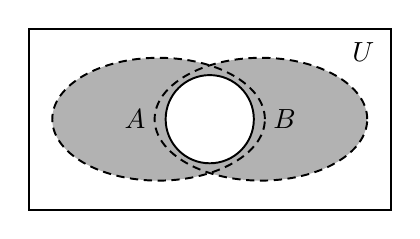
\begin{tikzpicture}[scale=1,line width=0.7pt]
\draw (0,0) rectangle (4.6,2.3);
\fill[black!30] (1.65,1.15) ellipse (1.35 and 0.78);
\fill[black!30] (2.95,1.15) ellipse (1.35 and 0.78);
\fill[white] (2.3,1.15) circle (0.56);
\draw[densely dashed] (1.65,1.15) ellipse (1.35 and 0.78);
\draw[densely dashed] (2.95,1.15) ellipse (1.35 and 0.78);
\draw (2.3,1.15) circle (0.56);
\node at (1.35,1.15) {$A$};
\node at (3.25,1.15) {$B$};
\node at (4.25,2.0) {$U$};
\end{tikzpicture}
\end{center}

\keepwithprev
A. $(-2,1)$\qquad B. $[-1,0]\cup[1,2)$\qquad C. $(-2,-1)\cup[0,1]$\qquad D. $[0,1]$

\ifanswer
\solbegin
\step{$A=\{x\mid-2<x<0\}$，$B=\{x\mid-1\leqslant x\leqslant1\}$，}
\step{所以 $A\cap B=\{x\mid-1\leqslant x<0\}$，$A\cup B=\{x\mid-2<x\leqslant1\}$，}
\step{则图中阴影部分表示的集合是 $(-2,-1)\cup[0,1]$，故选 $C$.}
\solend
\fi

\item 用反证法证明：“若 $x$、$y\in\R$ 且 $x+y>2$，则 $x$、$y$ 中至少有一个大于 $1$”时，应假设\mbox{（\quad）}% 原卷括号内已印“D”，试卷版按惯例留空

\keepwithprev
A. $x$、$y$ 中至少有一个小于 $1$\qquad B. $x$、$y$ 均小于 $1$

C. $x$、$y$ 中至少有一个小于等于 $1$\qquad D. $x$、$y$ 均小于等于 $1$

\ifanswer
\ans{$D$}
\fi

\item 若关于 $x$ 的不等式 $ax^2+bx+c>0$ 的解集是 $(-1,2)$，则不等式 $\dfrac{3ax-b}{x-3}>0$ 的解集是\mbox{（\quad）}

\keepwithprev
A. $\left(-\infty,-\dfrac13\right)\cup(3,+\infty)$\qquad B. $\left(-\dfrac13,3\right)$

C. $(-\infty,-3)\cup\left(\dfrac13,+\infty\right)$\qquad D. $\left(-3,\dfrac13\right)$

\ifanswer
\solbegin
\step{因为不等式 $ax^2+bx+c>0$ 的解集是 $(-1,2)$，}
\step{所以 $-1$、$2$ 是方程 $ax^2+bx+c=0$ 的两个根，且 $a<0$，}
\step{所以 $\begin{cases}-1+2=-\dfrac ba\\ -1\times2=\dfrac ca\end{cases}\Rightarrow\begin{cases}b=-a\\ c=-2a\end{cases}$，}
\step{所以 $\dfrac{3ax-b}{x-3}>0\Rightarrow\dfrac{3ax+a}{x-3}>0\Leftrightarrow a(3x+1)(x-3)>0$，}
\step{又 $a<0$，所以 $(3x+1)(x-3)<0$，解得 $-\dfrac13<x<3$，}
\step{所以不等式 $\dfrac{3ax-b}{x-3}>0$ 的解集为 $\left(-\dfrac13,3\right)$，故选 $B$.}
\solend
\fi

\end{enumerate}

\bigsec{三、解答题}

\begin{enumerate}
\setcounter{enumi}{16}

\item 解下列不等式组：

（1）$\begin{cases}\dfrac{5-x}{x+3}>0\\ 2x-\lvert x-1\rvert>2\end{cases}$；\qquad（2）$\begin{cases}-x^2+x+6\geqslant0\\ \dfrac{x-2}{x+1}\geqslant0\end{cases}$.

\ansspace*[12]

\ifanswer
\solbegin
\stepm{（1）}{不等式 $\dfrac{5-x}{x+3}>0$ 等价于 $(x-5)(x+3)<0$，所以 $-3<x<5$，}
\step{不等式 $2x-\lvert x-1\rvert>2$ 等价于 $2x-2>\lvert x-1\rvert$，}
\step{所以 $2-2x<x-1<2x-2$，故 $x>1$，}
\step{所以不等式组的解集为 $(1,5)$；}
\stepm{（2）}{不等式组 $\begin{cases}-x^2+x+6\geqslant0\\ \dfrac{x-2}{x+1}\geqslant0\end{cases}$ 可化为 $\begin{cases}x^2-x-6\leqslant0\\ (x-2)(x+1)\geqslant0\\ x+1\neq0\end{cases}$，}
\step{解得 $\begin{cases}-2\leqslant x\leqslant3\\ x\leqslant-1\ \text{或}\ x\geqslant2\\ x\neq-1\end{cases}$，即 $-2\leqslant x<-1$ 或 $2\leqslant x\leqslant3$，}
\step{所以不等式组的解集为 $\{x\mid-2\leqslant x<-1$ 或 $2\leqslant x\leqslant3\}$.}
\solend
\fi

\needvspace{3.2cm}
\item 已知 $A=\{x\mid x^2-2x-3\leqslant0\}$，$B=\{x\mid a-1\leqslant x\leqslant2a+1\}$，$a\in\R$.

（1）若 $A\cap B=B$，求实数 $a$ 的取值范围.

（2）若 $a>b>0$，比较 $\dfrac{a^2-b^2}{a^2+b^2}$ 与 $\dfrac{a-b}{a+b}$ 的大小.

\ansspace*[13]

\ifanswer
\solbegin
\stepm{（1）}{解不等式 $x^2-2x-3\leqslant0$，得 $-1\leqslant x\leqslant3$，}
\step{因为 $A\cap B=B$，所以 $B\subseteq A$，}
\step{当 $B=\varnothing$ 时，则 $a-1>2a+1$，解得 $a<-2$，}
\step{当 $B\neq\varnothing$ 时，要使得 $B\subseteq A$，则满足 $\begin{cases}a-1\leqslant2a+1\\ a-1\geqslant-1\\ 2a+1\leqslant3\end{cases}$，解得 $0\leqslant a\leqslant1$，}
\step{综上，实数 $a$ 的取值范围为 $(-\infty,-2)\cup[0,1]$.}
\stepm{（2）}{因为 $a>b>0$，所以 $a-b>0$，$a+b>0$，$ab>0$，}
\step{所以 $a^2-b^2=(a-b)(a+b)>0$，$a^2+b^2+2ab>a^2+b^2>0$，}
\step{$\dfrac{a^2-b^2}{a^2+b^2}>0$，$\dfrac{a-b}{a+b}>0$，}
\step{$\dfrac{\dfrac{a^2-b^2}{a^2+b^2}}{\dfrac{a-b}{a+b}}=\dfrac{(a-b)(a+b)}{a^2+b^2}\cdot\dfrac{a+b}{a-b}=\dfrac{a^2+b^2+2ab}{a^2+b^2}>1$，}
\step{所以 $\dfrac{a^2-b^2}{a^2+b^2}>\dfrac{a-b}{a+b}$.}
\solend
\fi

\item 汽车在行驶中，由于惯性作用，刹车后还要继续向前滑行一段距离才能停住，我们称这段距离为“刹车距离”. 刹车距离是分析事故的一个重要因素. 在一个限速 $40\mathrm{km}/\mathrm{h}$ 以内的弯道上，甲、乙两辆汽车相向而行，发现情况不对，同时刹车，但还是相碰了，事发后现场测得甲车的刹车距离略超过 $12\mathrm{m}$，乙车的刹车距离略超过 $10\mathrm{m}$，又知甲、乙两种车型的刹车距离 $s(\mathrm{m})$ 与车速 $x(\mathrm{km}/\mathrm{h})$ 之间有如下关系：$s_{\text{甲}}=0.1x+0.01x^2$，$s_{\text{乙}}=0.05x+0.005x^2$. 问：两车相撞的主要责任是谁？

\ansspace*[10]

\ifanswer
\solbegin
\step{由题意列出不等式组 $\begin{cases}0.1x+0.01x^2>12\\ 0.05x+0.005x^2>10\end{cases}$，解得 $\begin{cases}x<-40\ \text{或}\ x>30\\ x<-50\ \text{或}\ x>40\end{cases}$，}
\step{由于 $x>0$，从而可得 $x_{\text{甲}}>30\mathrm{km}/\mathrm{h}$，$x_{\text{乙}}>40\mathrm{km}/\mathrm{h}$.}
\step{经比较得乙车超过限速，应负主要责任.}
\solend
\fi

\item 已知关于 $x$ 的一元二次方程 $x^2+(2m-1)x+m^2-3=0$ 有实数根.

（1）若方程有两个负根，求实数 $m$ 的取值范围；

（2）当 $m=2$ 时，记方程的根为 $x_1$、$x_2$，求代数式 $\lvert x_1-x_2\rvert$ 的值.

\ansspace*[12]

\ifanswer
\solbegin
\stepm{（1）}{由方程有两个负根，得 $\begin{cases}\Delta=(2m-1)^2-4(m^2-3)\geqslant0\\ -(2m-1)<0\\ m^2-3>0\end{cases}$，}
\step{即 $\begin{cases}13-4m\geqslant0\\ 2m-1>0\\ (m-\sqrt3)(m+\sqrt3)>0\end{cases}$，解得 $\sqrt3<m\leqslant\dfrac{13}4$，}
\step{则实数 $m$ 的取值范围为 $\left\{m\left|\sqrt3<m\leqslant\dfrac{13}4\right.\right\}$.}
\stepm{（2）}{当 $m=2$ 时，方程为 $x^2+3x+1=0$，}
\step{此时 $\Delta=3^2-4=5>0$，且 $x_1+x_2=-3$，$x_1x_2=1$，}
\step{则 $\lvert x_1-x_2\rvert=\sqrt{(x_1+x_2)^2-4x_1x_2}=\sqrt{(-3)^2-4}=\sqrt5$.}
\solend
\fi

\item 已知不等式 $\lvert2x-a\rvert\leqslant b$ 的解集为 $A$，不等式 $mx^2-mx-1<0$ 的解集为 $B$.

（1）若 $a=1$，$b=2$，求 $A$.

（2）若 $A=[-1,3]$，求实数 $a$、$b$ 的取值；

（3）若 $B=\R$，求实数 $m$ 的取值范围.

\ansspace*[12]

\ifanswer
\solbegin
\stepm{（1）}{因为 $a=1$，$b=2$，所以不等式 $\lvert2x-a\rvert\leqslant b$ 等价于 $\lvert2x-1\rvert\leqslant2$，}
\step{所以 $-2\leqslant2x-1\leqslant2$，故 $-\dfrac12\leqslant x\leqslant\dfrac32$，所以 $A=\left[-\dfrac12,\dfrac32\right]$；}
\stepm{（2）}{当 $b>0$ 时，不等式 $\lvert2x-a\rvert\leqslant b$ 可化为 $-b\leqslant2x-a\leqslant b$，}
\step{所以 $\dfrac{a-b}2\leqslant x\leqslant\dfrac{a+b}2$，由 $A=[-1,3]$，得 $\dfrac{a-b}2=-1$，$\dfrac{a+b}2=3$；}
\step{当 $b=0$ 时，不等式 $\lvert2x-a\rvert\leqslant b$ 的解集为 $\left\{\dfrac a2\right\}$，不满足要求，}
\step{当 $b<0$ 时，不等式 $\lvert2x-a\rvert\leqslant b$ 的解集为 $\varnothing$，不满足要求，}
\step{所以 $a=2$，$b=4$；}
\stepm{（3）}{由已知不等式 $mx^2-mx-1<0$ 的解集为 $\R$，}
\step{得 $\begin{cases}m<0\\ m^2+4m<0\end{cases}$ 或 $m=0$，解得 $-4<m<0$ 或 $m=0$，}
\step{所以实数 $m$ 的取值范围为 $(-4,0]$.}
\solend
\fi

\end{enumerate}

\end{document}
"
%
% 原始材料：微信公众号“魔都数学加油站”文章，连载“27学年高一97”；
% 原文标题“27学年高一97——2026-2027年上海市浦东中学高一上10月月考”；
% 原文链接：https://mp.weixin.qq.com/s/2uW3LikOX3B07IWw7LkF_g。
% 正文为 8 张 PNG 页（`原图/高一97_浦东中学_10月月考/01..08.png`）：04、08 为
% 2560×3620，其余为 4762×6735，按页序读取。
%
% 篇幅与题号：原卷自第 3 题起编号（第 1、2 题不在原文内）。填空题 3—12（10 题）、
% 选择题 13—16（4 题）、解答题 17—21（5 题），共 19 题。
%
% 讲评版：第 15 题无【解析】、答案“D”直接印在题干括号内，本稿试卷版按惯例留空、
% 答案版提 \ans{}；其余 18 题印【解析】，其中第 13、14、16 题的答案在解析末句
% “故选 $B$／$C$／$B$”。
%
% 副标题：原卷未印副标题。本稿按内容标作“集合与常用逻辑用语、不等式”。
%
% 插图：第 14 题题干右侧有一幅韦恩图（全集 $U$ 的矩形内两个相交椭圆 $A$、$B$，
% 阴影为两椭圆的对称差）。原图该页为 2560×3620 的低分辨率页，直接裁切会糊，
% 故按原图布局用 TikZ 重绘（三版都出）。
%
% 与原卷的排版差异：
%   ① 原卷每题下直接印【答案】/【解析】，本稿按全稿惯例将答案与解析置于答案版；
%   ② 原卷未印副标题，本稿补出；填空横线统一排 \blankline[4.4em]；
%   ③ 原卷数集记号排斜体 $R$，本稿按全稿惯例改用 $\R$；
%   ④ 第 14 题的韦恩图原为行内右侧小图，本稿改为居中单列；
%   ⑤ 解答题按惯例加 \ansspace；选择题括号排 \mbox{（\quad）}。
%
% 行数核对：逐题数 \step/\stepm 条数，合计 85 条（Q3：2；Q4：2；Q5：2；Q6：2；
% Q7：2；Q8：4；Q9：4；Q10：5；Q11：10；Q12：3；Q13：4；Q14：3；Q15：0；
% Q16：6；Q17：7；Q18：10；Q19：3；Q20：6；Q21：10）。第 15 题无解析，
% 不计入 \step 账。原卷解析的换行按语意合并，未逐行强拆。
%
\documentclass[a4paper,11pt]{article}
\usepackage{common}

\begin{document}

\examtitlest[2]{2026--2027 年浦东中学高一上 10 月月考}{集合与常用逻辑用语、不等式}

\bigsec{一、填空题}

\begin{enumerate}
\setcounter{enumi}{2}

\item “$a(a-2)<0$”是“$\dfrac2a>1$”成立的\blankline[4.4em]条件（填充分必要性）.

\ifanswer
\solbegin
\step{“不等式 $a(a-2)<0\Rightarrow0<a<2$，不等式 $\dfrac2a>1\Rightarrow\dfrac{2-a}a>0\Rightarrow0<a<2$，}
\step{两不等式解集相等，所以“$a(a-2)<0$”是“$\dfrac2a>1$”成立的充要条件.}
\solend
\fi

\item 求不等式 $\lvert5-2x\rvert\leqslant3$ 的解集\blankline[4.4em].

\ifanswer
\solbegin
\step{$\lvert5-2x\rvert\leqslant3$ 等价于 $-3\leqslant5-2x\leqslant3$，解得 $1\leqslant x\leqslant4$，}
\step{所以不等式 $\lvert5-2x\rvert\leqslant3$ 的解集为 $\{x\mid1\leqslant x\leqslant4\}$.}
\solend
\fi

\item 求不等式组 $\begin{cases}3x^2+2x-1<0\\ \dfrac1x\geqslant0\end{cases}$ 的解集\blankline[4.4em].

\ifanswer
\solbegin
\step{不等式 $3x^2+2x-1=(3x-1)(x+1)<0$，解得 $-1<x<\dfrac13$，}
\step{由不等式 $\dfrac1x\geqslant0$ 解得 $x>0$，所以不等式组的解集为 $\left(0,\dfrac13\right)$.}
\solend
\fi

\item 满足 $\{1,3\}\subseteq A\subseteq\{0,1,3,5\}$ 的所有集合 $A$ 的全部元素之和为\blankline[4.4em].

\ifanswer
\solbegin
\step{符合条件的集合 $A$ 有以下几个，$A_1=\{0,1,3\}$，$A_2=\{1,3,5\}$，$A_3=\{0,1,3,5\}$，}
\step{所以所有集合 $A$ 的全部元素之和为 $0+1+3+1+3+5+0+1+3+5=22$.}
\solend
\fi

\item 已知集合 $A=\{(x,y)\mid y=-x+1\}$，$B=\{(x,y)\mid y=x^2-1\}$，则 $A\cap B=\blankline[4.4em]$.

\ifanswer
\solbegin
\step{联立 $\begin{cases}y=-x+1\\ y=x^2-1\end{cases}$，解得 $\begin{cases}x=1\\ y=0\end{cases}$ 或 $\begin{cases}x=-2\\ y=3\end{cases}$，}
\step{故 $A\cap B=\{(1,0),(-2,3)\}$.}
\solend
\fi

\item 若 $a$、$b$ 是方程 $x^2+2x-3=0$ 的两个实数根，则 $a^2-2b=\blankline[4.4em]$.

\ifanswer
\solbegin
\step{$a$、$b$ 是方程 $x^2+2x-3=0$ 的两个实数根，}
\step{所以 $a^2+2a-3=0$，故 $a^2=3-2a$，}
\step{由韦达定理得 $a+b=-2$，所以 $b=-2-a$，}
\step{所以 $a^2-2b=3-2a-2b=3-2a+4+2a=7$.}
\solend
\fi

\item 设 $a$、$b$ 为实数，若不等式 $x^2-ax-b<0$ 的解集为 $(2,8)$，则 $bx^2-ax-1>0$ 的解集为\blankline[4.4em].

\ifanswer
\solbegin
\step{因为不等式 $x^2-ax-b<0$ 的解集为 $(2,8)$，所以 $\begin{cases}2+8=a\\ 2\times8=-b\end{cases}$，}
\step{所以 $a=10$，$b=-16$，所以 $bx^2-ax-1>0$ 可化为 $-16x^2-10x-1>0$，}
\step{所以 $16x^2+10x+1<0$，}
\step{所以所求不等式的解集为 $\left(-\dfrac12,-\dfrac18\right)$.}
\solend
\fi

\item 若集合 $A=\{x\mid x^2+3x-4=0\}$，$B=\{x\mid ax-1=0\}$，若 $A\cap B=B$，则实数 $a$ 的取值组成的集合是\blankline[4.4em].

\ifanswer
\solbegin
\step{集合 $A=\{x\mid x^2+3x-4=0\}=\{-4,1\}$，$B=\{x\mid ax-1=0\}$，}
\step{因为 $A\cap B=B$，所以 $B\subseteq A$，}
\step{当 $a=0$ 时，$B=\varnothing$，$B\subseteq A$ 成立；}
\step{当 $a\neq0$ 时，$B=\left\{\dfrac1a\right\}$，由 $B\subseteq A$，得 $\dfrac1a=-4$ 或 $\dfrac1a=1$，解得 $a=-\dfrac14$ 或 $a=1$，}
\step{所以实数 $a$ 的值为 $-\dfrac14$ 或 $0$ 或 $1$，实数 $a$ 的取值组成的集合是 $\left\{-\dfrac14,0,1\right\}$.}
\solend
\fi

\item 关于 $x$ 的不等式 $ax^2+(1-2a^2)x-2a<0$ 的解集中恰有 $3$ 个正整数解，则 $a$ 的取值范围为\blankline[4.4em].

\ifanswer
\solbegin
\step{①当 $a=0$ 时，不等式化为 $x<0$，则解集中有无数个整数，不满足题意；}
\step{当 $a\neq0$ 时，不等式 $ax^2+(1-2a^2)x-2a<0$ 的解集中恰有 $3$ 个正整数解，}
\step{即为不等式 $(ax+1)(x-2a)<0$ 的解集中恰有 $3$ 个正整数解，}
\step{②当 $a<0$ 时，不等式 $(ax+1)(x-2a)<0$ 的解集中有无数个正整数，}
\step{不满足题意，}
\step{③当 $a>0$ 时，$-\dfrac1a<0,2a>0$，所以 $-\dfrac1a<2a$，}
\step{所以不等式的解集为 $\left\{x\left|-\dfrac1a<x<2a\right.\right\}$，}
\step{由解集得 $0$ 一定属于此集合，则由不等式的解集中恰有 $3$ 个正整数，}
\step{则这 $3$ 个正整数一定为 $1$，$2$，$3$，则 $3<2a\leqslant4$，解得 $\dfrac32<a\leqslant2$，}
\step{所以 $a$ 的取值范围是 $\left\{a\left|\dfrac32<a\leqslant2\right.\right\}$.}
\solend
\fi

\item 设 $x\in\R$，$[x]$ 表示不大于 $x$ 的最大整数，如 $[\pi]=3$，$[-1.2]=-2$，$\left[\dfrac12\right]=0$，则使 $[\lvert x-1\rvert]=3$ 成立的 $x$ 的取值范围\blankline[4.4em].

\ifanswer
\solbegin
\step{由题意 $[\lvert x-1\rvert]=3$，则 $3\leqslant\lvert x-1\rvert<4$，所以 $3\leqslant x-1<4$ 或 $-4\leqslant x-1<-3$，}
\step{解得 $4\leqslant x<5$ 或 $-3<x\leqslant-2$，}
\step{所以使 $[\lvert x-1\rvert]=3$ 成立的 $x$ 的取值范围是 $(-3,-2]\cup[4,5)$.}
\solend
\fi

\end{enumerate}

\bigsec{二、选择题}

\begin{enumerate}
\setcounter{enumi}{12}

\item 若 $a\in\R$，则“$a^2>a$”是“$a>1$”的\mbox{（\quad）}

\keepwithprev
A. 充分非必要条件\qquad B. 必要非充分条件

C. 充要条件\qquad D. 既非充分又非必要条件

\ifanswer
\solbegin
\step{已知 $a^2>a$，则 $a(a-1)>0$，即 $a<0$ 或 $a>1$，}
\step{由“$a<0$ 或 $a>1$”不能推出“$a>1$”；}
\step{由“$a>1$”可以推出“$a<0$ 或 $a>1$”，即“$a>1$”可以推出“$a^2>a$”；}
\step{所以“$a^2>a$”是“$a>1$”的必要非充分条件. 故选 $B$.}
\solend
\fi

\item 已知全集 $U=\R$，集合 $A=\{x\mid x(x+2)<0\}$，$B=\{x\mid\lvert x\rvert\leqslant1\}$，则图中阴影部分表示的集合是\mbox{（\quad）}

\begin{center}
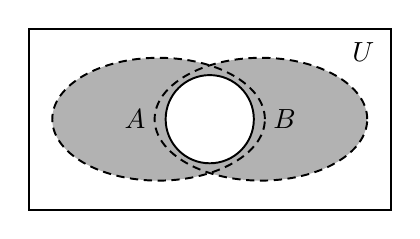
\begin{tikzpicture}[scale=1,line width=0.7pt]
\draw (0,0) rectangle (4.6,2.3);
\fill[black!30] (1.65,1.15) ellipse (1.35 and 0.78);
\fill[black!30] (2.95,1.15) ellipse (1.35 and 0.78);
\fill[white] (2.3,1.15) circle (0.56);
\draw[densely dashed] (1.65,1.15) ellipse (1.35 and 0.78);
\draw[densely dashed] (2.95,1.15) ellipse (1.35 and 0.78);
\draw (2.3,1.15) circle (0.56);
\node at (1.35,1.15) {$A$};
\node at (3.25,1.15) {$B$};
\node at (4.25,2.0) {$U$};
\end{tikzpicture}
\end{center}

\keepwithprev
A. $(-2,1)$\qquad B. $[-1,0]\cup[1,2)$\qquad C. $(-2,-1)\cup[0,1]$\qquad D. $[0,1]$

\ifanswer
\solbegin
\step{$A=\{x\mid-2<x<0\}$，$B=\{x\mid-1\leqslant x\leqslant1\}$，}
\step{所以 $A\cap B=\{x\mid-1\leqslant x<0\}$，$A\cup B=\{x\mid-2<x\leqslant1\}$，}
\step{则图中阴影部分表示的集合是 $(-2,-1)\cup[0,1]$，故选 $C$.}
\solend
\fi

\item 用反证法证明：“若 $x$、$y\in\R$ 且 $x+y>2$，则 $x$、$y$ 中至少有一个大于 $1$”时，应假设\mbox{（\quad）}% 原卷括号内已印“D”，试卷版按惯例留空

\keepwithprev
A. $x$、$y$ 中至少有一个小于 $1$\qquad B. $x$、$y$ 均小于 $1$

C. $x$、$y$ 中至少有一个小于等于 $1$\qquad D. $x$、$y$ 均小于等于 $1$

\ifanswer
\ans{$D$}
\fi

\item 若关于 $x$ 的不等式 $ax^2+bx+c>0$ 的解集是 $(-1,2)$，则不等式 $\dfrac{3ax-b}{x-3}>0$ 的解集是\mbox{（\quad）}

\keepwithprev
A. $\left(-\infty,-\dfrac13\right)\cup(3,+\infty)$\qquad B. $\left(-\dfrac13,3\right)$

C. $(-\infty,-3)\cup\left(\dfrac13,+\infty\right)$\qquad D. $\left(-3,\dfrac13\right)$

\ifanswer
\solbegin
\step{因为不等式 $ax^2+bx+c>0$ 的解集是 $(-1,2)$，}
\step{所以 $-1$、$2$ 是方程 $ax^2+bx+c=0$ 的两个根，且 $a<0$，}
\step{所以 $\begin{cases}-1+2=-\dfrac ba\\ -1\times2=\dfrac ca\end{cases}\Rightarrow\begin{cases}b=-a\\ c=-2a\end{cases}$，}
\step{所以 $\dfrac{3ax-b}{x-3}>0\Rightarrow\dfrac{3ax+a}{x-3}>0\Leftrightarrow a(3x+1)(x-3)>0$，}
\step{又 $a<0$，所以 $(3x+1)(x-3)<0$，解得 $-\dfrac13<x<3$，}
\step{所以不等式 $\dfrac{3ax-b}{x-3}>0$ 的解集为 $\left(-\dfrac13,3\right)$，故选 $B$.}
\solend
\fi

\end{enumerate}

\bigsec{三、解答题}

\begin{enumerate}
\setcounter{enumi}{16}

\item 解下列不等式组：

（1）$\begin{cases}\dfrac{5-x}{x+3}>0\\ 2x-\lvert x-1\rvert>2\end{cases}$；\qquad（2）$\begin{cases}-x^2+x+6\geqslant0\\ \dfrac{x-2}{x+1}\geqslant0\end{cases}$.

\ansspace*[12]

\ifanswer
\solbegin
\stepm{（1）}{不等式 $\dfrac{5-x}{x+3}>0$ 等价于 $(x-5)(x+3)<0$，所以 $-3<x<5$，}
\step{不等式 $2x-\lvert x-1\rvert>2$ 等价于 $2x-2>\lvert x-1\rvert$，}
\step{所以 $2-2x<x-1<2x-2$，故 $x>1$，}
\step{所以不等式组的解集为 $(1,5)$；}
\stepm{（2）}{不等式组 $\begin{cases}-x^2+x+6\geqslant0\\ \dfrac{x-2}{x+1}\geqslant0\end{cases}$ 可化为 $\begin{cases}x^2-x-6\leqslant0\\ (x-2)(x+1)\geqslant0\\ x+1\neq0\end{cases}$，}
\step{解得 $\begin{cases}-2\leqslant x\leqslant3\\ x\leqslant-1\ \text{或}\ x\geqslant2\\ x\neq-1\end{cases}$，即 $-2\leqslant x<-1$ 或 $2\leqslant x\leqslant3$，}
\step{所以不等式组的解集为 $\{x\mid-2\leqslant x<-1$ 或 $2\leqslant x\leqslant3\}$.}
\solend
\fi

\needvspace{3.2cm}
\item 已知 $A=\{x\mid x^2-2x-3\leqslant0\}$，$B=\{x\mid a-1\leqslant x\leqslant2a+1\}$，$a\in\R$.

（1）若 $A\cap B=B$，求实数 $a$ 的取值范围.

（2）若 $a>b>0$，比较 $\dfrac{a^2-b^2}{a^2+b^2}$ 与 $\dfrac{a-b}{a+b}$ 的大小.

\ansspace*[13]

\ifanswer
\solbegin
\stepm{（1）}{解不等式 $x^2-2x-3\leqslant0$，得 $-1\leqslant x\leqslant3$，}
\step{因为 $A\cap B=B$，所以 $B\subseteq A$，}
\step{当 $B=\varnothing$ 时，则 $a-1>2a+1$，解得 $a<-2$，}
\step{当 $B\neq\varnothing$ 时，要使得 $B\subseteq A$，则满足 $\begin{cases}a-1\leqslant2a+1\\ a-1\geqslant-1\\ 2a+1\leqslant3\end{cases}$，解得 $0\leqslant a\leqslant1$，}
\step{综上，实数 $a$ 的取值范围为 $(-\infty,-2)\cup[0,1]$.}
\stepm{（2）}{因为 $a>b>0$，所以 $a-b>0$，$a+b>0$，$ab>0$，}
\step{所以 $a^2-b^2=(a-b)(a+b)>0$，$a^2+b^2+2ab>a^2+b^2>0$，}
\step{$\dfrac{a^2-b^2}{a^2+b^2}>0$，$\dfrac{a-b}{a+b}>0$，}
\step{$\dfrac{\dfrac{a^2-b^2}{a^2+b^2}}{\dfrac{a-b}{a+b}}=\dfrac{(a-b)(a+b)}{a^2+b^2}\cdot\dfrac{a+b}{a-b}=\dfrac{a^2+b^2+2ab}{a^2+b^2}>1$，}
\step{所以 $\dfrac{a^2-b^2}{a^2+b^2}>\dfrac{a-b}{a+b}$.}
\solend
\fi

\item 汽车在行驶中，由于惯性作用，刹车后还要继续向前滑行一段距离才能停住，我们称这段距离为“刹车距离”. 刹车距离是分析事故的一个重要因素. 在一个限速 $40\mathrm{km}/\mathrm{h}$ 以内的弯道上，甲、乙两辆汽车相向而行，发现情况不对，同时刹车，但还是相碰了，事发后现场测得甲车的刹车距离略超过 $12\mathrm{m}$，乙车的刹车距离略超过 $10\mathrm{m}$，又知甲、乙两种车型的刹车距离 $s(\mathrm{m})$ 与车速 $x(\mathrm{km}/\mathrm{h})$ 之间有如下关系：$s_{\text{甲}}=0.1x+0.01x^2$，$s_{\text{乙}}=0.05x+0.005x^2$. 问：两车相撞的主要责任是谁？

\ansspace*[10]

\ifanswer
\solbegin
\step{由题意列出不等式组 $\begin{cases}0.1x+0.01x^2>12\\ 0.05x+0.005x^2>10\end{cases}$，解得 $\begin{cases}x<-40\ \text{或}\ x>30\\ x<-50\ \text{或}\ x>40\end{cases}$，}
\step{由于 $x>0$，从而可得 $x_{\text{甲}}>30\mathrm{km}/\mathrm{h}$，$x_{\text{乙}}>40\mathrm{km}/\mathrm{h}$.}
\step{经比较得乙车超过限速，应负主要责任.}
\solend
\fi

\item 已知关于 $x$ 的一元二次方程 $x^2+(2m-1)x+m^2-3=0$ 有实数根.

（1）若方程有两个负根，求实数 $m$ 的取值范围；

（2）当 $m=2$ 时，记方程的根为 $x_1$、$x_2$，求代数式 $\lvert x_1-x_2\rvert$ 的值.

\ansspace*[12]

\ifanswer
\solbegin
\stepm{（1）}{由方程有两个负根，得 $\begin{cases}\Delta=(2m-1)^2-4(m^2-3)\geqslant0\\ -(2m-1)<0\\ m^2-3>0\end{cases}$，}
\step{即 $\begin{cases}13-4m\geqslant0\\ 2m-1>0\\ (m-\sqrt3)(m+\sqrt3)>0\end{cases}$，解得 $\sqrt3<m\leqslant\dfrac{13}4$，}
\step{则实数 $m$ 的取值范围为 $\left\{m\left|\sqrt3<m\leqslant\dfrac{13}4\right.\right\}$.}
\stepm{（2）}{当 $m=2$ 时，方程为 $x^2+3x+1=0$，}
\step{此时 $\Delta=3^2-4=5>0$，且 $x_1+x_2=-3$，$x_1x_2=1$，}
\step{则 $\lvert x_1-x_2\rvert=\sqrt{(x_1+x_2)^2-4x_1x_2}=\sqrt{(-3)^2-4}=\sqrt5$.}
\solend
\fi

\item 已知不等式 $\lvert2x-a\rvert\leqslant b$ 的解集为 $A$，不等式 $mx^2-mx-1<0$ 的解集为 $B$.

（1）若 $a=1$，$b=2$，求 $A$.

（2）若 $A=[-1,3]$，求实数 $a$、$b$ 的取值；

（3）若 $B=\R$，求实数 $m$ 的取值范围.

\ansspace*[12]

\ifanswer
\solbegin
\stepm{（1）}{因为 $a=1$，$b=2$，所以不等式 $\lvert2x-a\rvert\leqslant b$ 等价于 $\lvert2x-1\rvert\leqslant2$，}
\step{所以 $-2\leqslant2x-1\leqslant2$，故 $-\dfrac12\leqslant x\leqslant\dfrac32$，所以 $A=\left[-\dfrac12,\dfrac32\right]$；}
\stepm{（2）}{当 $b>0$ 时，不等式 $\lvert2x-a\rvert\leqslant b$ 可化为 $-b\leqslant2x-a\leqslant b$，}
\step{所以 $\dfrac{a-b}2\leqslant x\leqslant\dfrac{a+b}2$，由 $A=[-1,3]$，得 $\dfrac{a-b}2=-1$，$\dfrac{a+b}2=3$；}
\step{当 $b=0$ 时，不等式 $\lvert2x-a\rvert\leqslant b$ 的解集为 $\left\{\dfrac a2\right\}$，不满足要求，}
\step{当 $b<0$ 时，不等式 $\lvert2x-a\rvert\leqslant b$ 的解集为 $\varnothing$，不满足要求，}
\step{所以 $a=2$，$b=4$；}
\stepm{（3）}{由已知不等式 $mx^2-mx-1<0$ 的解集为 $\R$，}
\step{得 $\begin{cases}m<0\\ m^2+4m<0\end{cases}$ 或 $m=0$，解得 $-4<m<0$ 或 $m=0$，}
\step{所以实数 $m$ 的取值范围为 $(-4,0]$.}
\solend
\fi

\end{enumerate}

\end{document}
"
% 紧凑版：xelatex "\def\iscompact{1}% 高一97_浦东中学_10月月考.tex
%   —— 高一上数学“2026-2027 年浦东中学高一上 10 月月考”（讲评版）
% 试卷版：xelatex 高一97_浦东中学_10月月考.tex
% 答案版：xelatex "\def\isanswer{1}% 高一97_浦东中学_10月月考.tex
%   —— 高一上数学“2026-2027 年浦东中学高一上 10 月月考”（讲评版）
% 试卷版：xelatex 高一97_浦东中学_10月月考.tex
% 答案版：xelatex "\def\isanswer{1}% 高一97_浦东中学_10月月考.tex
%   —— 高一上数学“2026-2027 年浦东中学高一上 10 月月考”（讲评版）
% 试卷版：xelatex 高一97_浦东中学_10月月考.tex
% 答案版：xelatex "\def\isanswer{1}\input{高一97_浦东中学_10月月考.tex}"
% 紧凑版：xelatex "\def\iscompact{1}\input{高一97_浦东中学_10月月考.tex}"
%
% 原始材料：微信公众号“魔都数学加油站”文章，连载“27学年高一97”；
% 原文标题“27学年高一97——2026-2027年上海市浦东中学高一上10月月考”；
% 原文链接：https://mp.weixin.qq.com/s/2uW3LikOX3B07IWw7LkF_g。
% 正文为 8 张 PNG 页（`原图/高一97_浦东中学_10月月考/01..08.png`）：04、08 为
% 2560×3620，其余为 4762×6735，按页序读取。
%
% 篇幅与题号：原卷自第 3 题起编号（第 1、2 题不在原文内）。填空题 3—12（10 题）、
% 选择题 13—16（4 题）、解答题 17—21（5 题），共 19 题。
%
% 讲评版：第 15 题无【解析】、答案“D”直接印在题干括号内，本稿试卷版按惯例留空、
% 答案版提 \ans{}；其余 18 题印【解析】，其中第 13、14、16 题的答案在解析末句
% “故选 $B$／$C$／$B$”。
%
% 副标题：原卷未印副标题。本稿按内容标作“集合与常用逻辑用语、不等式”。
%
% 插图：第 14 题题干右侧有一幅韦恩图（全集 $U$ 的矩形内两个相交椭圆 $A$、$B$，
% 阴影为两椭圆的对称差）。原图该页为 2560×3620 的低分辨率页，直接裁切会糊，
% 故按原图布局用 TikZ 重绘（三版都出）。
%
% 与原卷的排版差异：
%   ① 原卷每题下直接印【答案】/【解析】，本稿按全稿惯例将答案与解析置于答案版；
%   ② 原卷未印副标题，本稿补出；填空横线统一排 \blankline[4.4em]；
%   ③ 原卷数集记号排斜体 $R$，本稿按全稿惯例改用 $\R$；
%   ④ 第 14 题的韦恩图原为行内右侧小图，本稿改为居中单列；
%   ⑤ 解答题按惯例加 \ansspace；选择题括号排 \mbox{（\quad）}。
%
% 行数核对：逐题数 \step/\stepm 条数，合计 85 条（Q3：2；Q4：2；Q5：2；Q6：2；
% Q7：2；Q8：4；Q9：4；Q10：5；Q11：10；Q12：3；Q13：4；Q14：3；Q15：0；
% Q16：6；Q17：7；Q18：10；Q19：3；Q20：6；Q21：10）。第 15 题无解析，
% 不计入 \step 账。原卷解析的换行按语意合并，未逐行强拆。
%
\documentclass[a4paper,11pt]{article}
\usepackage{common}

\begin{document}

\examtitlest[2]{2026--2027 年浦东中学高一上 10 月月考}{集合与常用逻辑用语、不等式}

\bigsec{一、填空题}

\begin{enumerate}
\setcounter{enumi}{2}

\item “$a(a-2)<0$”是“$\dfrac2a>1$”成立的\blankline[4.4em]条件（填充分必要性）.

\ifanswer
\solbegin
\step{“不等式 $a(a-2)<0\Rightarrow0<a<2$，不等式 $\dfrac2a>1\Rightarrow\dfrac{2-a}a>0\Rightarrow0<a<2$，}
\step{两不等式解集相等，所以“$a(a-2)<0$”是“$\dfrac2a>1$”成立的充要条件.}
\solend
\fi

\item 求不等式 $\lvert5-2x\rvert\leqslant3$ 的解集\blankline[4.4em].

\ifanswer
\solbegin
\step{$\lvert5-2x\rvert\leqslant3$ 等价于 $-3\leqslant5-2x\leqslant3$，解得 $1\leqslant x\leqslant4$，}
\step{所以不等式 $\lvert5-2x\rvert\leqslant3$ 的解集为 $\{x\mid1\leqslant x\leqslant4\}$.}
\solend
\fi

\item 求不等式组 $\begin{cases}3x^2+2x-1<0\\ \dfrac1x\geqslant0\end{cases}$ 的解集\blankline[4.4em].

\ifanswer
\solbegin
\step{不等式 $3x^2+2x-1=(3x-1)(x+1)<0$，解得 $-1<x<\dfrac13$，}
\step{由不等式 $\dfrac1x\geqslant0$ 解得 $x>0$，所以不等式组的解集为 $\left(0,\dfrac13\right)$.}
\solend
\fi

\item 满足 $\{1,3\}\subseteq A\subseteq\{0,1,3,5\}$ 的所有集合 $A$ 的全部元素之和为\blankline[4.4em].

\ifanswer
\solbegin
\step{符合条件的集合 $A$ 有以下几个，$A_1=\{0,1,3\}$，$A_2=\{1,3,5\}$，$A_3=\{0,1,3,5\}$，}
\step{所以所有集合 $A$ 的全部元素之和为 $0+1+3+1+3+5+0+1+3+5=22$.}
\solend
\fi

\item 已知集合 $A=\{(x,y)\mid y=-x+1\}$，$B=\{(x,y)\mid y=x^2-1\}$，则 $A\cap B=\blankline[4.4em]$.

\ifanswer
\solbegin
\step{联立 $\begin{cases}y=-x+1\\ y=x^2-1\end{cases}$，解得 $\begin{cases}x=1\\ y=0\end{cases}$ 或 $\begin{cases}x=-2\\ y=3\end{cases}$，}
\step{故 $A\cap B=\{(1,0),(-2,3)\}$.}
\solend
\fi

\item 若 $a$、$b$ 是方程 $x^2+2x-3=0$ 的两个实数根，则 $a^2-2b=\blankline[4.4em]$.

\ifanswer
\solbegin
\step{$a$、$b$ 是方程 $x^2+2x-3=0$ 的两个实数根，}
\step{所以 $a^2+2a-3=0$，故 $a^2=3-2a$，}
\step{由韦达定理得 $a+b=-2$，所以 $b=-2-a$，}
\step{所以 $a^2-2b=3-2a-2b=3-2a+4+2a=7$.}
\solend
\fi

\item 设 $a$、$b$ 为实数，若不等式 $x^2-ax-b<0$ 的解集为 $(2,8)$，则 $bx^2-ax-1>0$ 的解集为\blankline[4.4em].

\ifanswer
\solbegin
\step{因为不等式 $x^2-ax-b<0$ 的解集为 $(2,8)$，所以 $\begin{cases}2+8=a\\ 2\times8=-b\end{cases}$，}
\step{所以 $a=10$，$b=-16$，所以 $bx^2-ax-1>0$ 可化为 $-16x^2-10x-1>0$，}
\step{所以 $16x^2+10x+1<0$，}
\step{所以所求不等式的解集为 $\left(-\dfrac12,-\dfrac18\right)$.}
\solend
\fi

\item 若集合 $A=\{x\mid x^2+3x-4=0\}$，$B=\{x\mid ax-1=0\}$，若 $A\cap B=B$，则实数 $a$ 的取值组成的集合是\blankline[4.4em].

\ifanswer
\solbegin
\step{集合 $A=\{x\mid x^2+3x-4=0\}=\{-4,1\}$，$B=\{x\mid ax-1=0\}$，}
\step{因为 $A\cap B=B$，所以 $B\subseteq A$，}
\step{当 $a=0$ 时，$B=\varnothing$，$B\subseteq A$ 成立；}
\step{当 $a\neq0$ 时，$B=\left\{\dfrac1a\right\}$，由 $B\subseteq A$，得 $\dfrac1a=-4$ 或 $\dfrac1a=1$，解得 $a=-\dfrac14$ 或 $a=1$，}
\step{所以实数 $a$ 的值为 $-\dfrac14$ 或 $0$ 或 $1$，实数 $a$ 的取值组成的集合是 $\left\{-\dfrac14,0,1\right\}$.}
\solend
\fi

\item 关于 $x$ 的不等式 $ax^2+(1-2a^2)x-2a<0$ 的解集中恰有 $3$ 个正整数解，则 $a$ 的取值范围为\blankline[4.4em].

\ifanswer
\solbegin
\step{①当 $a=0$ 时，不等式化为 $x<0$，则解集中有无数个整数，不满足题意；}
\step{当 $a\neq0$ 时，不等式 $ax^2+(1-2a^2)x-2a<0$ 的解集中恰有 $3$ 个正整数解，}
\step{即为不等式 $(ax+1)(x-2a)<0$ 的解集中恰有 $3$ 个正整数解，}
\step{②当 $a<0$ 时，不等式 $(ax+1)(x-2a)<0$ 的解集中有无数个正整数，}
\step{不满足题意，}
\step{③当 $a>0$ 时，$-\dfrac1a<0,2a>0$，所以 $-\dfrac1a<2a$，}
\step{所以不等式的解集为 $\left\{x\left|-\dfrac1a<x<2a\right.\right\}$，}
\step{由解集得 $0$ 一定属于此集合，则由不等式的解集中恰有 $3$ 个正整数，}
\step{则这 $3$ 个正整数一定为 $1$，$2$，$3$，则 $3<2a\leqslant4$，解得 $\dfrac32<a\leqslant2$，}
\step{所以 $a$ 的取值范围是 $\left\{a\left|\dfrac32<a\leqslant2\right.\right\}$.}
\solend
\fi

\item 设 $x\in\R$，$[x]$ 表示不大于 $x$ 的最大整数，如 $[\pi]=3$，$[-1.2]=-2$，$\left[\dfrac12\right]=0$，则使 $[\lvert x-1\rvert]=3$ 成立的 $x$ 的取值范围\blankline[4.4em].

\ifanswer
\solbegin
\step{由题意 $[\lvert x-1\rvert]=3$，则 $3\leqslant\lvert x-1\rvert<4$，所以 $3\leqslant x-1<4$ 或 $-4\leqslant x-1<-3$，}
\step{解得 $4\leqslant x<5$ 或 $-3<x\leqslant-2$，}
\step{所以使 $[\lvert x-1\rvert]=3$ 成立的 $x$ 的取值范围是 $(-3,-2]\cup[4,5)$.}
\solend
\fi

\end{enumerate}

\bigsec{二、选择题}

\begin{enumerate}
\setcounter{enumi}{12}

\item 若 $a\in\R$，则“$a^2>a$”是“$a>1$”的\mbox{（\quad）}

\keepwithprev
A. 充分非必要条件\qquad B. 必要非充分条件

C. 充要条件\qquad D. 既非充分又非必要条件

\ifanswer
\solbegin
\step{已知 $a^2>a$，则 $a(a-1)>0$，即 $a<0$ 或 $a>1$，}
\step{由“$a<0$ 或 $a>1$”不能推出“$a>1$”；}
\step{由“$a>1$”可以推出“$a<0$ 或 $a>1$”，即“$a>1$”可以推出“$a^2>a$”；}
\step{所以“$a^2>a$”是“$a>1$”的必要非充分条件. 故选 $B$.}
\solend
\fi

\item 已知全集 $U=\R$，集合 $A=\{x\mid x(x+2)<0\}$，$B=\{x\mid\lvert x\rvert\leqslant1\}$，则图中阴影部分表示的集合是\mbox{（\quad）}

\begin{center}
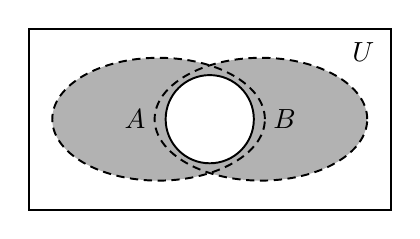
\begin{tikzpicture}[scale=1,line width=0.7pt]
\draw (0,0) rectangle (4.6,2.3);
\fill[black!30] (1.65,1.15) ellipse (1.35 and 0.78);
\fill[black!30] (2.95,1.15) ellipse (1.35 and 0.78);
\fill[white] (2.3,1.15) circle (0.56);
\draw[densely dashed] (1.65,1.15) ellipse (1.35 and 0.78);
\draw[densely dashed] (2.95,1.15) ellipse (1.35 and 0.78);
\draw (2.3,1.15) circle (0.56);
\node at (1.35,1.15) {$A$};
\node at (3.25,1.15) {$B$};
\node at (4.25,2.0) {$U$};
\end{tikzpicture}
\end{center}

\keepwithprev
A. $(-2,1)$\qquad B. $[-1,0]\cup[1,2)$\qquad C. $(-2,-1)\cup[0,1]$\qquad D. $[0,1]$

\ifanswer
\solbegin
\step{$A=\{x\mid-2<x<0\}$，$B=\{x\mid-1\leqslant x\leqslant1\}$，}
\step{所以 $A\cap B=\{x\mid-1\leqslant x<0\}$，$A\cup B=\{x\mid-2<x\leqslant1\}$，}
\step{则图中阴影部分表示的集合是 $(-2,-1)\cup[0,1]$，故选 $C$.}
\solend
\fi

\item 用反证法证明：“若 $x$、$y\in\R$ 且 $x+y>2$，则 $x$、$y$ 中至少有一个大于 $1$”时，应假设\mbox{（\quad）}% 原卷括号内已印“D”，试卷版按惯例留空

\keepwithprev
A. $x$、$y$ 中至少有一个小于 $1$\qquad B. $x$、$y$ 均小于 $1$

C. $x$、$y$ 中至少有一个小于等于 $1$\qquad D. $x$、$y$ 均小于等于 $1$

\ifanswer
\ans{$D$}
\fi

\item 若关于 $x$ 的不等式 $ax^2+bx+c>0$ 的解集是 $(-1,2)$，则不等式 $\dfrac{3ax-b}{x-3}>0$ 的解集是\mbox{（\quad）}

\keepwithprev
A. $\left(-\infty,-\dfrac13\right)\cup(3,+\infty)$\qquad B. $\left(-\dfrac13,3\right)$

C. $(-\infty,-3)\cup\left(\dfrac13,+\infty\right)$\qquad D. $\left(-3,\dfrac13\right)$

\ifanswer
\solbegin
\step{因为不等式 $ax^2+bx+c>0$ 的解集是 $(-1,2)$，}
\step{所以 $-1$、$2$ 是方程 $ax^2+bx+c=0$ 的两个根，且 $a<0$，}
\step{所以 $\begin{cases}-1+2=-\dfrac ba\\ -1\times2=\dfrac ca\end{cases}\Rightarrow\begin{cases}b=-a\\ c=-2a\end{cases}$，}
\step{所以 $\dfrac{3ax-b}{x-3}>0\Rightarrow\dfrac{3ax+a}{x-3}>0\Leftrightarrow a(3x+1)(x-3)>0$，}
\step{又 $a<0$，所以 $(3x+1)(x-3)<0$，解得 $-\dfrac13<x<3$，}
\step{所以不等式 $\dfrac{3ax-b}{x-3}>0$ 的解集为 $\left(-\dfrac13,3\right)$，故选 $B$.}
\solend
\fi

\end{enumerate}

\bigsec{三、解答题}

\begin{enumerate}
\setcounter{enumi}{16}

\item 解下列不等式组：

（1）$\begin{cases}\dfrac{5-x}{x+3}>0\\ 2x-\lvert x-1\rvert>2\end{cases}$；\qquad（2）$\begin{cases}-x^2+x+6\geqslant0\\ \dfrac{x-2}{x+1}\geqslant0\end{cases}$.

\ansspace*[12]

\ifanswer
\solbegin
\stepm{（1）}{不等式 $\dfrac{5-x}{x+3}>0$ 等价于 $(x-5)(x+3)<0$，所以 $-3<x<5$，}
\step{不等式 $2x-\lvert x-1\rvert>2$ 等价于 $2x-2>\lvert x-1\rvert$，}
\step{所以 $2-2x<x-1<2x-2$，故 $x>1$，}
\step{所以不等式组的解集为 $(1,5)$；}
\stepm{（2）}{不等式组 $\begin{cases}-x^2+x+6\geqslant0\\ \dfrac{x-2}{x+1}\geqslant0\end{cases}$ 可化为 $\begin{cases}x^2-x-6\leqslant0\\ (x-2)(x+1)\geqslant0\\ x+1\neq0\end{cases}$，}
\step{解得 $\begin{cases}-2\leqslant x\leqslant3\\ x\leqslant-1\ \text{或}\ x\geqslant2\\ x\neq-1\end{cases}$，即 $-2\leqslant x<-1$ 或 $2\leqslant x\leqslant3$，}
\step{所以不等式组的解集为 $\{x\mid-2\leqslant x<-1$ 或 $2\leqslant x\leqslant3\}$.}
\solend
\fi

\needvspace{3.2cm}
\item 已知 $A=\{x\mid x^2-2x-3\leqslant0\}$，$B=\{x\mid a-1\leqslant x\leqslant2a+1\}$，$a\in\R$.

（1）若 $A\cap B=B$，求实数 $a$ 的取值范围.

（2）若 $a>b>0$，比较 $\dfrac{a^2-b^2}{a^2+b^2}$ 与 $\dfrac{a-b}{a+b}$ 的大小.

\ansspace*[13]

\ifanswer
\solbegin
\stepm{（1）}{解不等式 $x^2-2x-3\leqslant0$，得 $-1\leqslant x\leqslant3$，}
\step{因为 $A\cap B=B$，所以 $B\subseteq A$，}
\step{当 $B=\varnothing$ 时，则 $a-1>2a+1$，解得 $a<-2$，}
\step{当 $B\neq\varnothing$ 时，要使得 $B\subseteq A$，则满足 $\begin{cases}a-1\leqslant2a+1\\ a-1\geqslant-1\\ 2a+1\leqslant3\end{cases}$，解得 $0\leqslant a\leqslant1$，}
\step{综上，实数 $a$ 的取值范围为 $(-\infty,-2)\cup[0,1]$.}
\stepm{（2）}{因为 $a>b>0$，所以 $a-b>0$，$a+b>0$，$ab>0$，}
\step{所以 $a^2-b^2=(a-b)(a+b)>0$，$a^2+b^2+2ab>a^2+b^2>0$，}
\step{$\dfrac{a^2-b^2}{a^2+b^2}>0$，$\dfrac{a-b}{a+b}>0$，}
\step{$\dfrac{\dfrac{a^2-b^2}{a^2+b^2}}{\dfrac{a-b}{a+b}}=\dfrac{(a-b)(a+b)}{a^2+b^2}\cdot\dfrac{a+b}{a-b}=\dfrac{a^2+b^2+2ab}{a^2+b^2}>1$，}
\step{所以 $\dfrac{a^2-b^2}{a^2+b^2}>\dfrac{a-b}{a+b}$.}
\solend
\fi

\item 汽车在行驶中，由于惯性作用，刹车后还要继续向前滑行一段距离才能停住，我们称这段距离为“刹车距离”. 刹车距离是分析事故的一个重要因素. 在一个限速 $40\mathrm{km}/\mathrm{h}$ 以内的弯道上，甲、乙两辆汽车相向而行，发现情况不对，同时刹车，但还是相碰了，事发后现场测得甲车的刹车距离略超过 $12\mathrm{m}$，乙车的刹车距离略超过 $10\mathrm{m}$，又知甲、乙两种车型的刹车距离 $s(\mathrm{m})$ 与车速 $x(\mathrm{km}/\mathrm{h})$ 之间有如下关系：$s_{\text{甲}}=0.1x+0.01x^2$，$s_{\text{乙}}=0.05x+0.005x^2$. 问：两车相撞的主要责任是谁？

\ansspace*[10]

\ifanswer
\solbegin
\step{由题意列出不等式组 $\begin{cases}0.1x+0.01x^2>12\\ 0.05x+0.005x^2>10\end{cases}$，解得 $\begin{cases}x<-40\ \text{或}\ x>30\\ x<-50\ \text{或}\ x>40\end{cases}$，}
\step{由于 $x>0$，从而可得 $x_{\text{甲}}>30\mathrm{km}/\mathrm{h}$，$x_{\text{乙}}>40\mathrm{km}/\mathrm{h}$.}
\step{经比较得乙车超过限速，应负主要责任.}
\solend
\fi

\item 已知关于 $x$ 的一元二次方程 $x^2+(2m-1)x+m^2-3=0$ 有实数根.

（1）若方程有两个负根，求实数 $m$ 的取值范围；

（2）当 $m=2$ 时，记方程的根为 $x_1$、$x_2$，求代数式 $\lvert x_1-x_2\rvert$ 的值.

\ansspace*[12]

\ifanswer
\solbegin
\stepm{（1）}{由方程有两个负根，得 $\begin{cases}\Delta=(2m-1)^2-4(m^2-3)\geqslant0\\ -(2m-1)<0\\ m^2-3>0\end{cases}$，}
\step{即 $\begin{cases}13-4m\geqslant0\\ 2m-1>0\\ (m-\sqrt3)(m+\sqrt3)>0\end{cases}$，解得 $\sqrt3<m\leqslant\dfrac{13}4$，}
\step{则实数 $m$ 的取值范围为 $\left\{m\left|\sqrt3<m\leqslant\dfrac{13}4\right.\right\}$.}
\stepm{（2）}{当 $m=2$ 时，方程为 $x^2+3x+1=0$，}
\step{此时 $\Delta=3^2-4=5>0$，且 $x_1+x_2=-3$，$x_1x_2=1$，}
\step{则 $\lvert x_1-x_2\rvert=\sqrt{(x_1+x_2)^2-4x_1x_2}=\sqrt{(-3)^2-4}=\sqrt5$.}
\solend
\fi

\item 已知不等式 $\lvert2x-a\rvert\leqslant b$ 的解集为 $A$，不等式 $mx^2-mx-1<0$ 的解集为 $B$.

（1）若 $a=1$，$b=2$，求 $A$.

（2）若 $A=[-1,3]$，求实数 $a$、$b$ 的取值；

（3）若 $B=\R$，求实数 $m$ 的取值范围.

\ansspace*[12]

\ifanswer
\solbegin
\stepm{（1）}{因为 $a=1$，$b=2$，所以不等式 $\lvert2x-a\rvert\leqslant b$ 等价于 $\lvert2x-1\rvert\leqslant2$，}
\step{所以 $-2\leqslant2x-1\leqslant2$，故 $-\dfrac12\leqslant x\leqslant\dfrac32$，所以 $A=\left[-\dfrac12,\dfrac32\right]$；}
\stepm{（2）}{当 $b>0$ 时，不等式 $\lvert2x-a\rvert\leqslant b$ 可化为 $-b\leqslant2x-a\leqslant b$，}
\step{所以 $\dfrac{a-b}2\leqslant x\leqslant\dfrac{a+b}2$，由 $A=[-1,3]$，得 $\dfrac{a-b}2=-1$，$\dfrac{a+b}2=3$；}
\step{当 $b=0$ 时，不等式 $\lvert2x-a\rvert\leqslant b$ 的解集为 $\left\{\dfrac a2\right\}$，不满足要求，}
\step{当 $b<0$ 时，不等式 $\lvert2x-a\rvert\leqslant b$ 的解集为 $\varnothing$，不满足要求，}
\step{所以 $a=2$，$b=4$；}
\stepm{（3）}{由已知不等式 $mx^2-mx-1<0$ 的解集为 $\R$，}
\step{得 $\begin{cases}m<0\\ m^2+4m<0\end{cases}$ 或 $m=0$，解得 $-4<m<0$ 或 $m=0$，}
\step{所以实数 $m$ 的取值范围为 $(-4,0]$.}
\solend
\fi

\end{enumerate}

\end{document}
"
% 紧凑版：xelatex "\def\iscompact{1}% 高一97_浦东中学_10月月考.tex
%   —— 高一上数学“2026-2027 年浦东中学高一上 10 月月考”（讲评版）
% 试卷版：xelatex 高一97_浦东中学_10月月考.tex
% 答案版：xelatex "\def\isanswer{1}\input{高一97_浦东中学_10月月考.tex}"
% 紧凑版：xelatex "\def\iscompact{1}\input{高一97_浦东中学_10月月考.tex}"
%
% 原始材料：微信公众号“魔都数学加油站”文章，连载“27学年高一97”；
% 原文标题“27学年高一97——2026-2027年上海市浦东中学高一上10月月考”；
% 原文链接：https://mp.weixin.qq.com/s/2uW3LikOX3B07IWw7LkF_g。
% 正文为 8 张 PNG 页（`原图/高一97_浦东中学_10月月考/01..08.png`）：04、08 为
% 2560×3620，其余为 4762×6735，按页序读取。
%
% 篇幅与题号：原卷自第 3 题起编号（第 1、2 题不在原文内）。填空题 3—12（10 题）、
% 选择题 13—16（4 题）、解答题 17—21（5 题），共 19 题。
%
% 讲评版：第 15 题无【解析】、答案“D”直接印在题干括号内，本稿试卷版按惯例留空、
% 答案版提 \ans{}；其余 18 题印【解析】，其中第 13、14、16 题的答案在解析末句
% “故选 $B$／$C$／$B$”。
%
% 副标题：原卷未印副标题。本稿按内容标作“集合与常用逻辑用语、不等式”。
%
% 插图：第 14 题题干右侧有一幅韦恩图（全集 $U$ 的矩形内两个相交椭圆 $A$、$B$，
% 阴影为两椭圆的对称差）。原图该页为 2560×3620 的低分辨率页，直接裁切会糊，
% 故按原图布局用 TikZ 重绘（三版都出）。
%
% 与原卷的排版差异：
%   ① 原卷每题下直接印【答案】/【解析】，本稿按全稿惯例将答案与解析置于答案版；
%   ② 原卷未印副标题，本稿补出；填空横线统一排 \blankline[4.4em]；
%   ③ 原卷数集记号排斜体 $R$，本稿按全稿惯例改用 $\R$；
%   ④ 第 14 题的韦恩图原为行内右侧小图，本稿改为居中单列；
%   ⑤ 解答题按惯例加 \ansspace；选择题括号排 \mbox{（\quad）}。
%
% 行数核对：逐题数 \step/\stepm 条数，合计 85 条（Q3：2；Q4：2；Q5：2；Q6：2；
% Q7：2；Q8：4；Q9：4；Q10：5；Q11：10；Q12：3；Q13：4；Q14：3；Q15：0；
% Q16：6；Q17：7；Q18：10；Q19：3；Q20：6；Q21：10）。第 15 题无解析，
% 不计入 \step 账。原卷解析的换行按语意合并，未逐行强拆。
%
\documentclass[a4paper,11pt]{article}
\usepackage{common}

\begin{document}

\examtitlest[2]{2026--2027 年浦东中学高一上 10 月月考}{集合与常用逻辑用语、不等式}

\bigsec{一、填空题}

\begin{enumerate}
\setcounter{enumi}{2}

\item “$a(a-2)<0$”是“$\dfrac2a>1$”成立的\blankline[4.4em]条件（填充分必要性）.

\ifanswer
\solbegin
\step{“不等式 $a(a-2)<0\Rightarrow0<a<2$，不等式 $\dfrac2a>1\Rightarrow\dfrac{2-a}a>0\Rightarrow0<a<2$，}
\step{两不等式解集相等，所以“$a(a-2)<0$”是“$\dfrac2a>1$”成立的充要条件.}
\solend
\fi

\item 求不等式 $\lvert5-2x\rvert\leqslant3$ 的解集\blankline[4.4em].

\ifanswer
\solbegin
\step{$\lvert5-2x\rvert\leqslant3$ 等价于 $-3\leqslant5-2x\leqslant3$，解得 $1\leqslant x\leqslant4$，}
\step{所以不等式 $\lvert5-2x\rvert\leqslant3$ 的解集为 $\{x\mid1\leqslant x\leqslant4\}$.}
\solend
\fi

\item 求不等式组 $\begin{cases}3x^2+2x-1<0\\ \dfrac1x\geqslant0\end{cases}$ 的解集\blankline[4.4em].

\ifanswer
\solbegin
\step{不等式 $3x^2+2x-1=(3x-1)(x+1)<0$，解得 $-1<x<\dfrac13$，}
\step{由不等式 $\dfrac1x\geqslant0$ 解得 $x>0$，所以不等式组的解集为 $\left(0,\dfrac13\right)$.}
\solend
\fi

\item 满足 $\{1,3\}\subseteq A\subseteq\{0,1,3,5\}$ 的所有集合 $A$ 的全部元素之和为\blankline[4.4em].

\ifanswer
\solbegin
\step{符合条件的集合 $A$ 有以下几个，$A_1=\{0,1,3\}$，$A_2=\{1,3,5\}$，$A_3=\{0,1,3,5\}$，}
\step{所以所有集合 $A$ 的全部元素之和为 $0+1+3+1+3+5+0+1+3+5=22$.}
\solend
\fi

\item 已知集合 $A=\{(x,y)\mid y=-x+1\}$，$B=\{(x,y)\mid y=x^2-1\}$，则 $A\cap B=\blankline[4.4em]$.

\ifanswer
\solbegin
\step{联立 $\begin{cases}y=-x+1\\ y=x^2-1\end{cases}$，解得 $\begin{cases}x=1\\ y=0\end{cases}$ 或 $\begin{cases}x=-2\\ y=3\end{cases}$，}
\step{故 $A\cap B=\{(1,0),(-2,3)\}$.}
\solend
\fi

\item 若 $a$、$b$ 是方程 $x^2+2x-3=0$ 的两个实数根，则 $a^2-2b=\blankline[4.4em]$.

\ifanswer
\solbegin
\step{$a$、$b$ 是方程 $x^2+2x-3=0$ 的两个实数根，}
\step{所以 $a^2+2a-3=0$，故 $a^2=3-2a$，}
\step{由韦达定理得 $a+b=-2$，所以 $b=-2-a$，}
\step{所以 $a^2-2b=3-2a-2b=3-2a+4+2a=7$.}
\solend
\fi

\item 设 $a$、$b$ 为实数，若不等式 $x^2-ax-b<0$ 的解集为 $(2,8)$，则 $bx^2-ax-1>0$ 的解集为\blankline[4.4em].

\ifanswer
\solbegin
\step{因为不等式 $x^2-ax-b<0$ 的解集为 $(2,8)$，所以 $\begin{cases}2+8=a\\ 2\times8=-b\end{cases}$，}
\step{所以 $a=10$，$b=-16$，所以 $bx^2-ax-1>0$ 可化为 $-16x^2-10x-1>0$，}
\step{所以 $16x^2+10x+1<0$，}
\step{所以所求不等式的解集为 $\left(-\dfrac12,-\dfrac18\right)$.}
\solend
\fi

\item 若集合 $A=\{x\mid x^2+3x-4=0\}$，$B=\{x\mid ax-1=0\}$，若 $A\cap B=B$，则实数 $a$ 的取值组成的集合是\blankline[4.4em].

\ifanswer
\solbegin
\step{集合 $A=\{x\mid x^2+3x-4=0\}=\{-4,1\}$，$B=\{x\mid ax-1=0\}$，}
\step{因为 $A\cap B=B$，所以 $B\subseteq A$，}
\step{当 $a=0$ 时，$B=\varnothing$，$B\subseteq A$ 成立；}
\step{当 $a\neq0$ 时，$B=\left\{\dfrac1a\right\}$，由 $B\subseteq A$，得 $\dfrac1a=-4$ 或 $\dfrac1a=1$，解得 $a=-\dfrac14$ 或 $a=1$，}
\step{所以实数 $a$ 的值为 $-\dfrac14$ 或 $0$ 或 $1$，实数 $a$ 的取值组成的集合是 $\left\{-\dfrac14,0,1\right\}$.}
\solend
\fi

\item 关于 $x$ 的不等式 $ax^2+(1-2a^2)x-2a<0$ 的解集中恰有 $3$ 个正整数解，则 $a$ 的取值范围为\blankline[4.4em].

\ifanswer
\solbegin
\step{①当 $a=0$ 时，不等式化为 $x<0$，则解集中有无数个整数，不满足题意；}
\step{当 $a\neq0$ 时，不等式 $ax^2+(1-2a^2)x-2a<0$ 的解集中恰有 $3$ 个正整数解，}
\step{即为不等式 $(ax+1)(x-2a)<0$ 的解集中恰有 $3$ 个正整数解，}
\step{②当 $a<0$ 时，不等式 $(ax+1)(x-2a)<0$ 的解集中有无数个正整数，}
\step{不满足题意，}
\step{③当 $a>0$ 时，$-\dfrac1a<0,2a>0$，所以 $-\dfrac1a<2a$，}
\step{所以不等式的解集为 $\left\{x\left|-\dfrac1a<x<2a\right.\right\}$，}
\step{由解集得 $0$ 一定属于此集合，则由不等式的解集中恰有 $3$ 个正整数，}
\step{则这 $3$ 个正整数一定为 $1$，$2$，$3$，则 $3<2a\leqslant4$，解得 $\dfrac32<a\leqslant2$，}
\step{所以 $a$ 的取值范围是 $\left\{a\left|\dfrac32<a\leqslant2\right.\right\}$.}
\solend
\fi

\item 设 $x\in\R$，$[x]$ 表示不大于 $x$ 的最大整数，如 $[\pi]=3$，$[-1.2]=-2$，$\left[\dfrac12\right]=0$，则使 $[\lvert x-1\rvert]=3$ 成立的 $x$ 的取值范围\blankline[4.4em].

\ifanswer
\solbegin
\step{由题意 $[\lvert x-1\rvert]=3$，则 $3\leqslant\lvert x-1\rvert<4$，所以 $3\leqslant x-1<4$ 或 $-4\leqslant x-1<-3$，}
\step{解得 $4\leqslant x<5$ 或 $-3<x\leqslant-2$，}
\step{所以使 $[\lvert x-1\rvert]=3$ 成立的 $x$ 的取值范围是 $(-3,-2]\cup[4,5)$.}
\solend
\fi

\end{enumerate}

\bigsec{二、选择题}

\begin{enumerate}
\setcounter{enumi}{12}

\item 若 $a\in\R$，则“$a^2>a$”是“$a>1$”的\mbox{（\quad）}

\keepwithprev
A. 充分非必要条件\qquad B. 必要非充分条件

C. 充要条件\qquad D. 既非充分又非必要条件

\ifanswer
\solbegin
\step{已知 $a^2>a$，则 $a(a-1)>0$，即 $a<0$ 或 $a>1$，}
\step{由“$a<0$ 或 $a>1$”不能推出“$a>1$”；}
\step{由“$a>1$”可以推出“$a<0$ 或 $a>1$”，即“$a>1$”可以推出“$a^2>a$”；}
\step{所以“$a^2>a$”是“$a>1$”的必要非充分条件. 故选 $B$.}
\solend
\fi

\item 已知全集 $U=\R$，集合 $A=\{x\mid x(x+2)<0\}$，$B=\{x\mid\lvert x\rvert\leqslant1\}$，则图中阴影部分表示的集合是\mbox{（\quad）}

\begin{center}
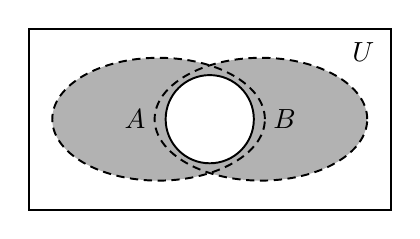
\begin{tikzpicture}[scale=1,line width=0.7pt]
\draw (0,0) rectangle (4.6,2.3);
\fill[black!30] (1.65,1.15) ellipse (1.35 and 0.78);
\fill[black!30] (2.95,1.15) ellipse (1.35 and 0.78);
\fill[white] (2.3,1.15) circle (0.56);
\draw[densely dashed] (1.65,1.15) ellipse (1.35 and 0.78);
\draw[densely dashed] (2.95,1.15) ellipse (1.35 and 0.78);
\draw (2.3,1.15) circle (0.56);
\node at (1.35,1.15) {$A$};
\node at (3.25,1.15) {$B$};
\node at (4.25,2.0) {$U$};
\end{tikzpicture}
\end{center}

\keepwithprev
A. $(-2,1)$\qquad B. $[-1,0]\cup[1,2)$\qquad C. $(-2,-1)\cup[0,1]$\qquad D. $[0,1]$

\ifanswer
\solbegin
\step{$A=\{x\mid-2<x<0\}$，$B=\{x\mid-1\leqslant x\leqslant1\}$，}
\step{所以 $A\cap B=\{x\mid-1\leqslant x<0\}$，$A\cup B=\{x\mid-2<x\leqslant1\}$，}
\step{则图中阴影部分表示的集合是 $(-2,-1)\cup[0,1]$，故选 $C$.}
\solend
\fi

\item 用反证法证明：“若 $x$、$y\in\R$ 且 $x+y>2$，则 $x$、$y$ 中至少有一个大于 $1$”时，应假设\mbox{（\quad）}% 原卷括号内已印“D”，试卷版按惯例留空

\keepwithprev
A. $x$、$y$ 中至少有一个小于 $1$\qquad B. $x$、$y$ 均小于 $1$

C. $x$、$y$ 中至少有一个小于等于 $1$\qquad D. $x$、$y$ 均小于等于 $1$

\ifanswer
\ans{$D$}
\fi

\item 若关于 $x$ 的不等式 $ax^2+bx+c>0$ 的解集是 $(-1,2)$，则不等式 $\dfrac{3ax-b}{x-3}>0$ 的解集是\mbox{（\quad）}

\keepwithprev
A. $\left(-\infty,-\dfrac13\right)\cup(3,+\infty)$\qquad B. $\left(-\dfrac13,3\right)$

C. $(-\infty,-3)\cup\left(\dfrac13,+\infty\right)$\qquad D. $\left(-3,\dfrac13\right)$

\ifanswer
\solbegin
\step{因为不等式 $ax^2+bx+c>0$ 的解集是 $(-1,2)$，}
\step{所以 $-1$、$2$ 是方程 $ax^2+bx+c=0$ 的两个根，且 $a<0$，}
\step{所以 $\begin{cases}-1+2=-\dfrac ba\\ -1\times2=\dfrac ca\end{cases}\Rightarrow\begin{cases}b=-a\\ c=-2a\end{cases}$，}
\step{所以 $\dfrac{3ax-b}{x-3}>0\Rightarrow\dfrac{3ax+a}{x-3}>0\Leftrightarrow a(3x+1)(x-3)>0$，}
\step{又 $a<0$，所以 $(3x+1)(x-3)<0$，解得 $-\dfrac13<x<3$，}
\step{所以不等式 $\dfrac{3ax-b}{x-3}>0$ 的解集为 $\left(-\dfrac13,3\right)$，故选 $B$.}
\solend
\fi

\end{enumerate}

\bigsec{三、解答题}

\begin{enumerate}
\setcounter{enumi}{16}

\item 解下列不等式组：

（1）$\begin{cases}\dfrac{5-x}{x+3}>0\\ 2x-\lvert x-1\rvert>2\end{cases}$；\qquad（2）$\begin{cases}-x^2+x+6\geqslant0\\ \dfrac{x-2}{x+1}\geqslant0\end{cases}$.

\ansspace*[12]

\ifanswer
\solbegin
\stepm{（1）}{不等式 $\dfrac{5-x}{x+3}>0$ 等价于 $(x-5)(x+3)<0$，所以 $-3<x<5$，}
\step{不等式 $2x-\lvert x-1\rvert>2$ 等价于 $2x-2>\lvert x-1\rvert$，}
\step{所以 $2-2x<x-1<2x-2$，故 $x>1$，}
\step{所以不等式组的解集为 $(1,5)$；}
\stepm{（2）}{不等式组 $\begin{cases}-x^2+x+6\geqslant0\\ \dfrac{x-2}{x+1}\geqslant0\end{cases}$ 可化为 $\begin{cases}x^2-x-6\leqslant0\\ (x-2)(x+1)\geqslant0\\ x+1\neq0\end{cases}$，}
\step{解得 $\begin{cases}-2\leqslant x\leqslant3\\ x\leqslant-1\ \text{或}\ x\geqslant2\\ x\neq-1\end{cases}$，即 $-2\leqslant x<-1$ 或 $2\leqslant x\leqslant3$，}
\step{所以不等式组的解集为 $\{x\mid-2\leqslant x<-1$ 或 $2\leqslant x\leqslant3\}$.}
\solend
\fi

\needvspace{3.2cm}
\item 已知 $A=\{x\mid x^2-2x-3\leqslant0\}$，$B=\{x\mid a-1\leqslant x\leqslant2a+1\}$，$a\in\R$.

（1）若 $A\cap B=B$，求实数 $a$ 的取值范围.

（2）若 $a>b>0$，比较 $\dfrac{a^2-b^2}{a^2+b^2}$ 与 $\dfrac{a-b}{a+b}$ 的大小.

\ansspace*[13]

\ifanswer
\solbegin
\stepm{（1）}{解不等式 $x^2-2x-3\leqslant0$，得 $-1\leqslant x\leqslant3$，}
\step{因为 $A\cap B=B$，所以 $B\subseteq A$，}
\step{当 $B=\varnothing$ 时，则 $a-1>2a+1$，解得 $a<-2$，}
\step{当 $B\neq\varnothing$ 时，要使得 $B\subseteq A$，则满足 $\begin{cases}a-1\leqslant2a+1\\ a-1\geqslant-1\\ 2a+1\leqslant3\end{cases}$，解得 $0\leqslant a\leqslant1$，}
\step{综上，实数 $a$ 的取值范围为 $(-\infty,-2)\cup[0,1]$.}
\stepm{（2）}{因为 $a>b>0$，所以 $a-b>0$，$a+b>0$，$ab>0$，}
\step{所以 $a^2-b^2=(a-b)(a+b)>0$，$a^2+b^2+2ab>a^2+b^2>0$，}
\step{$\dfrac{a^2-b^2}{a^2+b^2}>0$，$\dfrac{a-b}{a+b}>0$，}
\step{$\dfrac{\dfrac{a^2-b^2}{a^2+b^2}}{\dfrac{a-b}{a+b}}=\dfrac{(a-b)(a+b)}{a^2+b^2}\cdot\dfrac{a+b}{a-b}=\dfrac{a^2+b^2+2ab}{a^2+b^2}>1$，}
\step{所以 $\dfrac{a^2-b^2}{a^2+b^2}>\dfrac{a-b}{a+b}$.}
\solend
\fi

\item 汽车在行驶中，由于惯性作用，刹车后还要继续向前滑行一段距离才能停住，我们称这段距离为“刹车距离”. 刹车距离是分析事故的一个重要因素. 在一个限速 $40\mathrm{km}/\mathrm{h}$ 以内的弯道上，甲、乙两辆汽车相向而行，发现情况不对，同时刹车，但还是相碰了，事发后现场测得甲车的刹车距离略超过 $12\mathrm{m}$，乙车的刹车距离略超过 $10\mathrm{m}$，又知甲、乙两种车型的刹车距离 $s(\mathrm{m})$ 与车速 $x(\mathrm{km}/\mathrm{h})$ 之间有如下关系：$s_{\text{甲}}=0.1x+0.01x^2$，$s_{\text{乙}}=0.05x+0.005x^2$. 问：两车相撞的主要责任是谁？

\ansspace*[10]

\ifanswer
\solbegin
\step{由题意列出不等式组 $\begin{cases}0.1x+0.01x^2>12\\ 0.05x+0.005x^2>10\end{cases}$，解得 $\begin{cases}x<-40\ \text{或}\ x>30\\ x<-50\ \text{或}\ x>40\end{cases}$，}
\step{由于 $x>0$，从而可得 $x_{\text{甲}}>30\mathrm{km}/\mathrm{h}$，$x_{\text{乙}}>40\mathrm{km}/\mathrm{h}$.}
\step{经比较得乙车超过限速，应负主要责任.}
\solend
\fi

\item 已知关于 $x$ 的一元二次方程 $x^2+(2m-1)x+m^2-3=0$ 有实数根.

（1）若方程有两个负根，求实数 $m$ 的取值范围；

（2）当 $m=2$ 时，记方程的根为 $x_1$、$x_2$，求代数式 $\lvert x_1-x_2\rvert$ 的值.

\ansspace*[12]

\ifanswer
\solbegin
\stepm{（1）}{由方程有两个负根，得 $\begin{cases}\Delta=(2m-1)^2-4(m^2-3)\geqslant0\\ -(2m-1)<0\\ m^2-3>0\end{cases}$，}
\step{即 $\begin{cases}13-4m\geqslant0\\ 2m-1>0\\ (m-\sqrt3)(m+\sqrt3)>0\end{cases}$，解得 $\sqrt3<m\leqslant\dfrac{13}4$，}
\step{则实数 $m$ 的取值范围为 $\left\{m\left|\sqrt3<m\leqslant\dfrac{13}4\right.\right\}$.}
\stepm{（2）}{当 $m=2$ 时，方程为 $x^2+3x+1=0$，}
\step{此时 $\Delta=3^2-4=5>0$，且 $x_1+x_2=-3$，$x_1x_2=1$，}
\step{则 $\lvert x_1-x_2\rvert=\sqrt{(x_1+x_2)^2-4x_1x_2}=\sqrt{(-3)^2-4}=\sqrt5$.}
\solend
\fi

\item 已知不等式 $\lvert2x-a\rvert\leqslant b$ 的解集为 $A$，不等式 $mx^2-mx-1<0$ 的解集为 $B$.

（1）若 $a=1$，$b=2$，求 $A$.

（2）若 $A=[-1,3]$，求实数 $a$、$b$ 的取值；

（3）若 $B=\R$，求实数 $m$ 的取值范围.

\ansspace*[12]

\ifanswer
\solbegin
\stepm{（1）}{因为 $a=1$，$b=2$，所以不等式 $\lvert2x-a\rvert\leqslant b$ 等价于 $\lvert2x-1\rvert\leqslant2$，}
\step{所以 $-2\leqslant2x-1\leqslant2$，故 $-\dfrac12\leqslant x\leqslant\dfrac32$，所以 $A=\left[-\dfrac12,\dfrac32\right]$；}
\stepm{（2）}{当 $b>0$ 时，不等式 $\lvert2x-a\rvert\leqslant b$ 可化为 $-b\leqslant2x-a\leqslant b$，}
\step{所以 $\dfrac{a-b}2\leqslant x\leqslant\dfrac{a+b}2$，由 $A=[-1,3]$，得 $\dfrac{a-b}2=-1$，$\dfrac{a+b}2=3$；}
\step{当 $b=0$ 时，不等式 $\lvert2x-a\rvert\leqslant b$ 的解集为 $\left\{\dfrac a2\right\}$，不满足要求，}
\step{当 $b<0$ 时，不等式 $\lvert2x-a\rvert\leqslant b$ 的解集为 $\varnothing$，不满足要求，}
\step{所以 $a=2$，$b=4$；}
\stepm{（3）}{由已知不等式 $mx^2-mx-1<0$ 的解集为 $\R$，}
\step{得 $\begin{cases}m<0\\ m^2+4m<0\end{cases}$ 或 $m=0$，解得 $-4<m<0$ 或 $m=0$，}
\step{所以实数 $m$ 的取值范围为 $(-4,0]$.}
\solend
\fi

\end{enumerate}

\end{document}
"
%
% 原始材料：微信公众号“魔都数学加油站”文章，连载“27学年高一97”；
% 原文标题“27学年高一97——2026-2027年上海市浦东中学高一上10月月考”；
% 原文链接：https://mp.weixin.qq.com/s/2uW3LikOX3B07IWw7LkF_g。
% 正文为 8 张 PNG 页（`原图/高一97_浦东中学_10月月考/01..08.png`）：04、08 为
% 2560×3620，其余为 4762×6735，按页序读取。
%
% 篇幅与题号：原卷自第 3 题起编号（第 1、2 题不在原文内）。填空题 3—12（10 题）、
% 选择题 13—16（4 题）、解答题 17—21（5 题），共 19 题。
%
% 讲评版：第 15 题无【解析】、答案“D”直接印在题干括号内，本稿试卷版按惯例留空、
% 答案版提 \ans{}；其余 18 题印【解析】，其中第 13、14、16 题的答案在解析末句
% “故选 $B$／$C$／$B$”。
%
% 副标题：原卷未印副标题。本稿按内容标作“集合与常用逻辑用语、不等式”。
%
% 插图：第 14 题题干右侧有一幅韦恩图（全集 $U$ 的矩形内两个相交椭圆 $A$、$B$，
% 阴影为两椭圆的对称差）。原图该页为 2560×3620 的低分辨率页，直接裁切会糊，
% 故按原图布局用 TikZ 重绘（三版都出）。
%
% 与原卷的排版差异：
%   ① 原卷每题下直接印【答案】/【解析】，本稿按全稿惯例将答案与解析置于答案版；
%   ② 原卷未印副标题，本稿补出；填空横线统一排 \blankline[4.4em]；
%   ③ 原卷数集记号排斜体 $R$，本稿按全稿惯例改用 $\R$；
%   ④ 第 14 题的韦恩图原为行内右侧小图，本稿改为居中单列；
%   ⑤ 解答题按惯例加 \ansspace；选择题括号排 \mbox{（\quad）}。
%
% 行数核对：逐题数 \step/\stepm 条数，合计 85 条（Q3：2；Q4：2；Q5：2；Q6：2；
% Q7：2；Q8：4；Q9：4；Q10：5；Q11：10；Q12：3；Q13：4；Q14：3；Q15：0；
% Q16：6；Q17：7；Q18：10；Q19：3；Q20：6；Q21：10）。第 15 题无解析，
% 不计入 \step 账。原卷解析的换行按语意合并，未逐行强拆。
%
\documentclass[a4paper,11pt]{article}
\usepackage{common}

\begin{document}

\examtitlest[2]{2026--2027 年浦东中学高一上 10 月月考}{集合与常用逻辑用语、不等式}

\bigsec{一、填空题}

\begin{enumerate}
\setcounter{enumi}{2}

\item “$a(a-2)<0$”是“$\dfrac2a>1$”成立的\blankline[4.4em]条件（填充分必要性）.

\ifanswer
\solbegin
\step{“不等式 $a(a-2)<0\Rightarrow0<a<2$，不等式 $\dfrac2a>1\Rightarrow\dfrac{2-a}a>0\Rightarrow0<a<2$，}
\step{两不等式解集相等，所以“$a(a-2)<0$”是“$\dfrac2a>1$”成立的充要条件.}
\solend
\fi

\item 求不等式 $\lvert5-2x\rvert\leqslant3$ 的解集\blankline[4.4em].

\ifanswer
\solbegin
\step{$\lvert5-2x\rvert\leqslant3$ 等价于 $-3\leqslant5-2x\leqslant3$，解得 $1\leqslant x\leqslant4$，}
\step{所以不等式 $\lvert5-2x\rvert\leqslant3$ 的解集为 $\{x\mid1\leqslant x\leqslant4\}$.}
\solend
\fi

\item 求不等式组 $\begin{cases}3x^2+2x-1<0\\ \dfrac1x\geqslant0\end{cases}$ 的解集\blankline[4.4em].

\ifanswer
\solbegin
\step{不等式 $3x^2+2x-1=(3x-1)(x+1)<0$，解得 $-1<x<\dfrac13$，}
\step{由不等式 $\dfrac1x\geqslant0$ 解得 $x>0$，所以不等式组的解集为 $\left(0,\dfrac13\right)$.}
\solend
\fi

\item 满足 $\{1,3\}\subseteq A\subseteq\{0,1,3,5\}$ 的所有集合 $A$ 的全部元素之和为\blankline[4.4em].

\ifanswer
\solbegin
\step{符合条件的集合 $A$ 有以下几个，$A_1=\{0,1,3\}$，$A_2=\{1,3,5\}$，$A_3=\{0,1,3,5\}$，}
\step{所以所有集合 $A$ 的全部元素之和为 $0+1+3+1+3+5+0+1+3+5=22$.}
\solend
\fi

\item 已知集合 $A=\{(x,y)\mid y=-x+1\}$，$B=\{(x,y)\mid y=x^2-1\}$，则 $A\cap B=\blankline[4.4em]$.

\ifanswer
\solbegin
\step{联立 $\begin{cases}y=-x+1\\ y=x^2-1\end{cases}$，解得 $\begin{cases}x=1\\ y=0\end{cases}$ 或 $\begin{cases}x=-2\\ y=3\end{cases}$，}
\step{故 $A\cap B=\{(1,0),(-2,3)\}$.}
\solend
\fi

\item 若 $a$、$b$ 是方程 $x^2+2x-3=0$ 的两个实数根，则 $a^2-2b=\blankline[4.4em]$.

\ifanswer
\solbegin
\step{$a$、$b$ 是方程 $x^2+2x-3=0$ 的两个实数根，}
\step{所以 $a^2+2a-3=0$，故 $a^2=3-2a$，}
\step{由韦达定理得 $a+b=-2$，所以 $b=-2-a$，}
\step{所以 $a^2-2b=3-2a-2b=3-2a+4+2a=7$.}
\solend
\fi

\item 设 $a$、$b$ 为实数，若不等式 $x^2-ax-b<0$ 的解集为 $(2,8)$，则 $bx^2-ax-1>0$ 的解集为\blankline[4.4em].

\ifanswer
\solbegin
\step{因为不等式 $x^2-ax-b<0$ 的解集为 $(2,8)$，所以 $\begin{cases}2+8=a\\ 2\times8=-b\end{cases}$，}
\step{所以 $a=10$，$b=-16$，所以 $bx^2-ax-1>0$ 可化为 $-16x^2-10x-1>0$，}
\step{所以 $16x^2+10x+1<0$，}
\step{所以所求不等式的解集为 $\left(-\dfrac12,-\dfrac18\right)$.}
\solend
\fi

\item 若集合 $A=\{x\mid x^2+3x-4=0\}$，$B=\{x\mid ax-1=0\}$，若 $A\cap B=B$，则实数 $a$ 的取值组成的集合是\blankline[4.4em].

\ifanswer
\solbegin
\step{集合 $A=\{x\mid x^2+3x-4=0\}=\{-4,1\}$，$B=\{x\mid ax-1=0\}$，}
\step{因为 $A\cap B=B$，所以 $B\subseteq A$，}
\step{当 $a=0$ 时，$B=\varnothing$，$B\subseteq A$ 成立；}
\step{当 $a\neq0$ 时，$B=\left\{\dfrac1a\right\}$，由 $B\subseteq A$，得 $\dfrac1a=-4$ 或 $\dfrac1a=1$，解得 $a=-\dfrac14$ 或 $a=1$，}
\step{所以实数 $a$ 的值为 $-\dfrac14$ 或 $0$ 或 $1$，实数 $a$ 的取值组成的集合是 $\left\{-\dfrac14,0,1\right\}$.}
\solend
\fi

\item 关于 $x$ 的不等式 $ax^2+(1-2a^2)x-2a<0$ 的解集中恰有 $3$ 个正整数解，则 $a$ 的取值范围为\blankline[4.4em].

\ifanswer
\solbegin
\step{①当 $a=0$ 时，不等式化为 $x<0$，则解集中有无数个整数，不满足题意；}
\step{当 $a\neq0$ 时，不等式 $ax^2+(1-2a^2)x-2a<0$ 的解集中恰有 $3$ 个正整数解，}
\step{即为不等式 $(ax+1)(x-2a)<0$ 的解集中恰有 $3$ 个正整数解，}
\step{②当 $a<0$ 时，不等式 $(ax+1)(x-2a)<0$ 的解集中有无数个正整数，}
\step{不满足题意，}
\step{③当 $a>0$ 时，$-\dfrac1a<0,2a>0$，所以 $-\dfrac1a<2a$，}
\step{所以不等式的解集为 $\left\{x\left|-\dfrac1a<x<2a\right.\right\}$，}
\step{由解集得 $0$ 一定属于此集合，则由不等式的解集中恰有 $3$ 个正整数，}
\step{则这 $3$ 个正整数一定为 $1$，$2$，$3$，则 $3<2a\leqslant4$，解得 $\dfrac32<a\leqslant2$，}
\step{所以 $a$ 的取值范围是 $\left\{a\left|\dfrac32<a\leqslant2\right.\right\}$.}
\solend
\fi

\item 设 $x\in\R$，$[x]$ 表示不大于 $x$ 的最大整数，如 $[\pi]=3$，$[-1.2]=-2$，$\left[\dfrac12\right]=0$，则使 $[\lvert x-1\rvert]=3$ 成立的 $x$ 的取值范围\blankline[4.4em].

\ifanswer
\solbegin
\step{由题意 $[\lvert x-1\rvert]=3$，则 $3\leqslant\lvert x-1\rvert<4$，所以 $3\leqslant x-1<4$ 或 $-4\leqslant x-1<-3$，}
\step{解得 $4\leqslant x<5$ 或 $-3<x\leqslant-2$，}
\step{所以使 $[\lvert x-1\rvert]=3$ 成立的 $x$ 的取值范围是 $(-3,-2]\cup[4,5)$.}
\solend
\fi

\end{enumerate}

\bigsec{二、选择题}

\begin{enumerate}
\setcounter{enumi}{12}

\item 若 $a\in\R$，则“$a^2>a$”是“$a>1$”的\mbox{（\quad）}

\keepwithprev
A. 充分非必要条件\qquad B. 必要非充分条件

C. 充要条件\qquad D. 既非充分又非必要条件

\ifanswer
\solbegin
\step{已知 $a^2>a$，则 $a(a-1)>0$，即 $a<0$ 或 $a>1$，}
\step{由“$a<0$ 或 $a>1$”不能推出“$a>1$”；}
\step{由“$a>1$”可以推出“$a<0$ 或 $a>1$”，即“$a>1$”可以推出“$a^2>a$”；}
\step{所以“$a^2>a$”是“$a>1$”的必要非充分条件. 故选 $B$.}
\solend
\fi

\item 已知全集 $U=\R$，集合 $A=\{x\mid x(x+2)<0\}$，$B=\{x\mid\lvert x\rvert\leqslant1\}$，则图中阴影部分表示的集合是\mbox{（\quad）}

\begin{center}
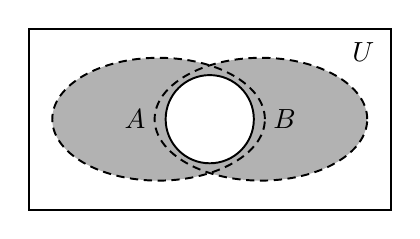
\begin{tikzpicture}[scale=1,line width=0.7pt]
\draw (0,0) rectangle (4.6,2.3);
\fill[black!30] (1.65,1.15) ellipse (1.35 and 0.78);
\fill[black!30] (2.95,1.15) ellipse (1.35 and 0.78);
\fill[white] (2.3,1.15) circle (0.56);
\draw[densely dashed] (1.65,1.15) ellipse (1.35 and 0.78);
\draw[densely dashed] (2.95,1.15) ellipse (1.35 and 0.78);
\draw (2.3,1.15) circle (0.56);
\node at (1.35,1.15) {$A$};
\node at (3.25,1.15) {$B$};
\node at (4.25,2.0) {$U$};
\end{tikzpicture}
\end{center}

\keepwithprev
A. $(-2,1)$\qquad B. $[-1,0]\cup[1,2)$\qquad C. $(-2,-1)\cup[0,1]$\qquad D. $[0,1]$

\ifanswer
\solbegin
\step{$A=\{x\mid-2<x<0\}$，$B=\{x\mid-1\leqslant x\leqslant1\}$，}
\step{所以 $A\cap B=\{x\mid-1\leqslant x<0\}$，$A\cup B=\{x\mid-2<x\leqslant1\}$，}
\step{则图中阴影部分表示的集合是 $(-2,-1)\cup[0,1]$，故选 $C$.}
\solend
\fi

\item 用反证法证明：“若 $x$、$y\in\R$ 且 $x+y>2$，则 $x$、$y$ 中至少有一个大于 $1$”时，应假设\mbox{（\quad）}% 原卷括号内已印“D”，试卷版按惯例留空

\keepwithprev
A. $x$、$y$ 中至少有一个小于 $1$\qquad B. $x$、$y$ 均小于 $1$

C. $x$、$y$ 中至少有一个小于等于 $1$\qquad D. $x$、$y$ 均小于等于 $1$

\ifanswer
\ans{$D$}
\fi

\item 若关于 $x$ 的不等式 $ax^2+bx+c>0$ 的解集是 $(-1,2)$，则不等式 $\dfrac{3ax-b}{x-3}>0$ 的解集是\mbox{（\quad）}

\keepwithprev
A. $\left(-\infty,-\dfrac13\right)\cup(3,+\infty)$\qquad B. $\left(-\dfrac13,3\right)$

C. $(-\infty,-3)\cup\left(\dfrac13,+\infty\right)$\qquad D. $\left(-3,\dfrac13\right)$

\ifanswer
\solbegin
\step{因为不等式 $ax^2+bx+c>0$ 的解集是 $(-1,2)$，}
\step{所以 $-1$、$2$ 是方程 $ax^2+bx+c=0$ 的两个根，且 $a<0$，}
\step{所以 $\begin{cases}-1+2=-\dfrac ba\\ -1\times2=\dfrac ca\end{cases}\Rightarrow\begin{cases}b=-a\\ c=-2a\end{cases}$，}
\step{所以 $\dfrac{3ax-b}{x-3}>0\Rightarrow\dfrac{3ax+a}{x-3}>0\Leftrightarrow a(3x+1)(x-3)>0$，}
\step{又 $a<0$，所以 $(3x+1)(x-3)<0$，解得 $-\dfrac13<x<3$，}
\step{所以不等式 $\dfrac{3ax-b}{x-3}>0$ 的解集为 $\left(-\dfrac13,3\right)$，故选 $B$.}
\solend
\fi

\end{enumerate}

\bigsec{三、解答题}

\begin{enumerate}
\setcounter{enumi}{16}

\item 解下列不等式组：

（1）$\begin{cases}\dfrac{5-x}{x+3}>0\\ 2x-\lvert x-1\rvert>2\end{cases}$；\qquad（2）$\begin{cases}-x^2+x+6\geqslant0\\ \dfrac{x-2}{x+1}\geqslant0\end{cases}$.

\ansspace*[12]

\ifanswer
\solbegin
\stepm{（1）}{不等式 $\dfrac{5-x}{x+3}>0$ 等价于 $(x-5)(x+3)<0$，所以 $-3<x<5$，}
\step{不等式 $2x-\lvert x-1\rvert>2$ 等价于 $2x-2>\lvert x-1\rvert$，}
\step{所以 $2-2x<x-1<2x-2$，故 $x>1$，}
\step{所以不等式组的解集为 $(1,5)$；}
\stepm{（2）}{不等式组 $\begin{cases}-x^2+x+6\geqslant0\\ \dfrac{x-2}{x+1}\geqslant0\end{cases}$ 可化为 $\begin{cases}x^2-x-6\leqslant0\\ (x-2)(x+1)\geqslant0\\ x+1\neq0\end{cases}$，}
\step{解得 $\begin{cases}-2\leqslant x\leqslant3\\ x\leqslant-1\ \text{或}\ x\geqslant2\\ x\neq-1\end{cases}$，即 $-2\leqslant x<-1$ 或 $2\leqslant x\leqslant3$，}
\step{所以不等式组的解集为 $\{x\mid-2\leqslant x<-1$ 或 $2\leqslant x\leqslant3\}$.}
\solend
\fi

\needvspace{3.2cm}
\item 已知 $A=\{x\mid x^2-2x-3\leqslant0\}$，$B=\{x\mid a-1\leqslant x\leqslant2a+1\}$，$a\in\R$.

（1）若 $A\cap B=B$，求实数 $a$ 的取值范围.

（2）若 $a>b>0$，比较 $\dfrac{a^2-b^2}{a^2+b^2}$ 与 $\dfrac{a-b}{a+b}$ 的大小.

\ansspace*[13]

\ifanswer
\solbegin
\stepm{（1）}{解不等式 $x^2-2x-3\leqslant0$，得 $-1\leqslant x\leqslant3$，}
\step{因为 $A\cap B=B$，所以 $B\subseteq A$，}
\step{当 $B=\varnothing$ 时，则 $a-1>2a+1$，解得 $a<-2$，}
\step{当 $B\neq\varnothing$ 时，要使得 $B\subseteq A$，则满足 $\begin{cases}a-1\leqslant2a+1\\ a-1\geqslant-1\\ 2a+1\leqslant3\end{cases}$，解得 $0\leqslant a\leqslant1$，}
\step{综上，实数 $a$ 的取值范围为 $(-\infty,-2)\cup[0,1]$.}
\stepm{（2）}{因为 $a>b>0$，所以 $a-b>0$，$a+b>0$，$ab>0$，}
\step{所以 $a^2-b^2=(a-b)(a+b)>0$，$a^2+b^2+2ab>a^2+b^2>0$，}
\step{$\dfrac{a^2-b^2}{a^2+b^2}>0$，$\dfrac{a-b}{a+b}>0$，}
\step{$\dfrac{\dfrac{a^2-b^2}{a^2+b^2}}{\dfrac{a-b}{a+b}}=\dfrac{(a-b)(a+b)}{a^2+b^2}\cdot\dfrac{a+b}{a-b}=\dfrac{a^2+b^2+2ab}{a^2+b^2}>1$，}
\step{所以 $\dfrac{a^2-b^2}{a^2+b^2}>\dfrac{a-b}{a+b}$.}
\solend
\fi

\item 汽车在行驶中，由于惯性作用，刹车后还要继续向前滑行一段距离才能停住，我们称这段距离为“刹车距离”. 刹车距离是分析事故的一个重要因素. 在一个限速 $40\mathrm{km}/\mathrm{h}$ 以内的弯道上，甲、乙两辆汽车相向而行，发现情况不对，同时刹车，但还是相碰了，事发后现场测得甲车的刹车距离略超过 $12\mathrm{m}$，乙车的刹车距离略超过 $10\mathrm{m}$，又知甲、乙两种车型的刹车距离 $s(\mathrm{m})$ 与车速 $x(\mathrm{km}/\mathrm{h})$ 之间有如下关系：$s_{\text{甲}}=0.1x+0.01x^2$，$s_{\text{乙}}=0.05x+0.005x^2$. 问：两车相撞的主要责任是谁？

\ansspace*[10]

\ifanswer
\solbegin
\step{由题意列出不等式组 $\begin{cases}0.1x+0.01x^2>12\\ 0.05x+0.005x^2>10\end{cases}$，解得 $\begin{cases}x<-40\ \text{或}\ x>30\\ x<-50\ \text{或}\ x>40\end{cases}$，}
\step{由于 $x>0$，从而可得 $x_{\text{甲}}>30\mathrm{km}/\mathrm{h}$，$x_{\text{乙}}>40\mathrm{km}/\mathrm{h}$.}
\step{经比较得乙车超过限速，应负主要责任.}
\solend
\fi

\item 已知关于 $x$ 的一元二次方程 $x^2+(2m-1)x+m^2-3=0$ 有实数根.

（1）若方程有两个负根，求实数 $m$ 的取值范围；

（2）当 $m=2$ 时，记方程的根为 $x_1$、$x_2$，求代数式 $\lvert x_1-x_2\rvert$ 的值.

\ansspace*[12]

\ifanswer
\solbegin
\stepm{（1）}{由方程有两个负根，得 $\begin{cases}\Delta=(2m-1)^2-4(m^2-3)\geqslant0\\ -(2m-1)<0\\ m^2-3>0\end{cases}$，}
\step{即 $\begin{cases}13-4m\geqslant0\\ 2m-1>0\\ (m-\sqrt3)(m+\sqrt3)>0\end{cases}$，解得 $\sqrt3<m\leqslant\dfrac{13}4$，}
\step{则实数 $m$ 的取值范围为 $\left\{m\left|\sqrt3<m\leqslant\dfrac{13}4\right.\right\}$.}
\stepm{（2）}{当 $m=2$ 时，方程为 $x^2+3x+1=0$，}
\step{此时 $\Delta=3^2-4=5>0$，且 $x_1+x_2=-3$，$x_1x_2=1$，}
\step{则 $\lvert x_1-x_2\rvert=\sqrt{(x_1+x_2)^2-4x_1x_2}=\sqrt{(-3)^2-4}=\sqrt5$.}
\solend
\fi

\item 已知不等式 $\lvert2x-a\rvert\leqslant b$ 的解集为 $A$，不等式 $mx^2-mx-1<0$ 的解集为 $B$.

（1）若 $a=1$，$b=2$，求 $A$.

（2）若 $A=[-1,3]$，求实数 $a$、$b$ 的取值；

（3）若 $B=\R$，求实数 $m$ 的取值范围.

\ansspace*[12]

\ifanswer
\solbegin
\stepm{（1）}{因为 $a=1$，$b=2$，所以不等式 $\lvert2x-a\rvert\leqslant b$ 等价于 $\lvert2x-1\rvert\leqslant2$，}
\step{所以 $-2\leqslant2x-1\leqslant2$，故 $-\dfrac12\leqslant x\leqslant\dfrac32$，所以 $A=\left[-\dfrac12,\dfrac32\right]$；}
\stepm{（2）}{当 $b>0$ 时，不等式 $\lvert2x-a\rvert\leqslant b$ 可化为 $-b\leqslant2x-a\leqslant b$，}
\step{所以 $\dfrac{a-b}2\leqslant x\leqslant\dfrac{a+b}2$，由 $A=[-1,3]$，得 $\dfrac{a-b}2=-1$，$\dfrac{a+b}2=3$；}
\step{当 $b=0$ 时，不等式 $\lvert2x-a\rvert\leqslant b$ 的解集为 $\left\{\dfrac a2\right\}$，不满足要求，}
\step{当 $b<0$ 时，不等式 $\lvert2x-a\rvert\leqslant b$ 的解集为 $\varnothing$，不满足要求，}
\step{所以 $a=2$，$b=4$；}
\stepm{（3）}{由已知不等式 $mx^2-mx-1<0$ 的解集为 $\R$，}
\step{得 $\begin{cases}m<0\\ m^2+4m<0\end{cases}$ 或 $m=0$，解得 $-4<m<0$ 或 $m=0$，}
\step{所以实数 $m$ 的取值范围为 $(-4,0]$.}
\solend
\fi

\end{enumerate}

\end{document}
"
% 紧凑版：xelatex "\def\iscompact{1}% 高一97_浦东中学_10月月考.tex
%   —— 高一上数学“2026-2027 年浦东中学高一上 10 月月考”（讲评版）
% 试卷版：xelatex 高一97_浦东中学_10月月考.tex
% 答案版：xelatex "\def\isanswer{1}% 高一97_浦东中学_10月月考.tex
%   —— 高一上数学“2026-2027 年浦东中学高一上 10 月月考”（讲评版）
% 试卷版：xelatex 高一97_浦东中学_10月月考.tex
% 答案版：xelatex "\def\isanswer{1}\input{高一97_浦东中学_10月月考.tex}"
% 紧凑版：xelatex "\def\iscompact{1}\input{高一97_浦东中学_10月月考.tex}"
%
% 原始材料：微信公众号“魔都数学加油站”文章，连载“27学年高一97”；
% 原文标题“27学年高一97——2026-2027年上海市浦东中学高一上10月月考”；
% 原文链接：https://mp.weixin.qq.com/s/2uW3LikOX3B07IWw7LkF_g。
% 正文为 8 张 PNG 页（`原图/高一97_浦东中学_10月月考/01..08.png`）：04、08 为
% 2560×3620，其余为 4762×6735，按页序读取。
%
% 篇幅与题号：原卷自第 3 题起编号（第 1、2 题不在原文内）。填空题 3—12（10 题）、
% 选择题 13—16（4 题）、解答题 17—21（5 题），共 19 题。
%
% 讲评版：第 15 题无【解析】、答案“D”直接印在题干括号内，本稿试卷版按惯例留空、
% 答案版提 \ans{}；其余 18 题印【解析】，其中第 13、14、16 题的答案在解析末句
% “故选 $B$／$C$／$B$”。
%
% 副标题：原卷未印副标题。本稿按内容标作“集合与常用逻辑用语、不等式”。
%
% 插图：第 14 题题干右侧有一幅韦恩图（全集 $U$ 的矩形内两个相交椭圆 $A$、$B$，
% 阴影为两椭圆的对称差）。原图该页为 2560×3620 的低分辨率页，直接裁切会糊，
% 故按原图布局用 TikZ 重绘（三版都出）。
%
% 与原卷的排版差异：
%   ① 原卷每题下直接印【答案】/【解析】，本稿按全稿惯例将答案与解析置于答案版；
%   ② 原卷未印副标题，本稿补出；填空横线统一排 \blankline[4.4em]；
%   ③ 原卷数集记号排斜体 $R$，本稿按全稿惯例改用 $\R$；
%   ④ 第 14 题的韦恩图原为行内右侧小图，本稿改为居中单列；
%   ⑤ 解答题按惯例加 \ansspace；选择题括号排 \mbox{（\quad）}。
%
% 行数核对：逐题数 \step/\stepm 条数，合计 85 条（Q3：2；Q4：2；Q5：2；Q6：2；
% Q7：2；Q8：4；Q9：4；Q10：5；Q11：10；Q12：3；Q13：4；Q14：3；Q15：0；
% Q16：6；Q17：7；Q18：10；Q19：3；Q20：6；Q21：10）。第 15 题无解析，
% 不计入 \step 账。原卷解析的换行按语意合并，未逐行强拆。
%
\documentclass[a4paper,11pt]{article}
\usepackage{common}

\begin{document}

\examtitlest[2]{2026--2027 年浦东中学高一上 10 月月考}{集合与常用逻辑用语、不等式}

\bigsec{一、填空题}

\begin{enumerate}
\setcounter{enumi}{2}

\item “$a(a-2)<0$”是“$\dfrac2a>1$”成立的\blankline[4.4em]条件（填充分必要性）.

\ifanswer
\solbegin
\step{“不等式 $a(a-2)<0\Rightarrow0<a<2$，不等式 $\dfrac2a>1\Rightarrow\dfrac{2-a}a>0\Rightarrow0<a<2$，}
\step{两不等式解集相等，所以“$a(a-2)<0$”是“$\dfrac2a>1$”成立的充要条件.}
\solend
\fi

\item 求不等式 $\lvert5-2x\rvert\leqslant3$ 的解集\blankline[4.4em].

\ifanswer
\solbegin
\step{$\lvert5-2x\rvert\leqslant3$ 等价于 $-3\leqslant5-2x\leqslant3$，解得 $1\leqslant x\leqslant4$，}
\step{所以不等式 $\lvert5-2x\rvert\leqslant3$ 的解集为 $\{x\mid1\leqslant x\leqslant4\}$.}
\solend
\fi

\item 求不等式组 $\begin{cases}3x^2+2x-1<0\\ \dfrac1x\geqslant0\end{cases}$ 的解集\blankline[4.4em].

\ifanswer
\solbegin
\step{不等式 $3x^2+2x-1=(3x-1)(x+1)<0$，解得 $-1<x<\dfrac13$，}
\step{由不等式 $\dfrac1x\geqslant0$ 解得 $x>0$，所以不等式组的解集为 $\left(0,\dfrac13\right)$.}
\solend
\fi

\item 满足 $\{1,3\}\subseteq A\subseteq\{0,1,3,5\}$ 的所有集合 $A$ 的全部元素之和为\blankline[4.4em].

\ifanswer
\solbegin
\step{符合条件的集合 $A$ 有以下几个，$A_1=\{0,1,3\}$，$A_2=\{1,3,5\}$，$A_3=\{0,1,3,5\}$，}
\step{所以所有集合 $A$ 的全部元素之和为 $0+1+3+1+3+5+0+1+3+5=22$.}
\solend
\fi

\item 已知集合 $A=\{(x,y)\mid y=-x+1\}$，$B=\{(x,y)\mid y=x^2-1\}$，则 $A\cap B=\blankline[4.4em]$.

\ifanswer
\solbegin
\step{联立 $\begin{cases}y=-x+1\\ y=x^2-1\end{cases}$，解得 $\begin{cases}x=1\\ y=0\end{cases}$ 或 $\begin{cases}x=-2\\ y=3\end{cases}$，}
\step{故 $A\cap B=\{(1,0),(-2,3)\}$.}
\solend
\fi

\item 若 $a$、$b$ 是方程 $x^2+2x-3=0$ 的两个实数根，则 $a^2-2b=\blankline[4.4em]$.

\ifanswer
\solbegin
\step{$a$、$b$ 是方程 $x^2+2x-3=0$ 的两个实数根，}
\step{所以 $a^2+2a-3=0$，故 $a^2=3-2a$，}
\step{由韦达定理得 $a+b=-2$，所以 $b=-2-a$，}
\step{所以 $a^2-2b=3-2a-2b=3-2a+4+2a=7$.}
\solend
\fi

\item 设 $a$、$b$ 为实数，若不等式 $x^2-ax-b<0$ 的解集为 $(2,8)$，则 $bx^2-ax-1>0$ 的解集为\blankline[4.4em].

\ifanswer
\solbegin
\step{因为不等式 $x^2-ax-b<0$ 的解集为 $(2,8)$，所以 $\begin{cases}2+8=a\\ 2\times8=-b\end{cases}$，}
\step{所以 $a=10$，$b=-16$，所以 $bx^2-ax-1>0$ 可化为 $-16x^2-10x-1>0$，}
\step{所以 $16x^2+10x+1<0$，}
\step{所以所求不等式的解集为 $\left(-\dfrac12,-\dfrac18\right)$.}
\solend
\fi

\item 若集合 $A=\{x\mid x^2+3x-4=0\}$，$B=\{x\mid ax-1=0\}$，若 $A\cap B=B$，则实数 $a$ 的取值组成的集合是\blankline[4.4em].

\ifanswer
\solbegin
\step{集合 $A=\{x\mid x^2+3x-4=0\}=\{-4,1\}$，$B=\{x\mid ax-1=0\}$，}
\step{因为 $A\cap B=B$，所以 $B\subseteq A$，}
\step{当 $a=0$ 时，$B=\varnothing$，$B\subseteq A$ 成立；}
\step{当 $a\neq0$ 时，$B=\left\{\dfrac1a\right\}$，由 $B\subseteq A$，得 $\dfrac1a=-4$ 或 $\dfrac1a=1$，解得 $a=-\dfrac14$ 或 $a=1$，}
\step{所以实数 $a$ 的值为 $-\dfrac14$ 或 $0$ 或 $1$，实数 $a$ 的取值组成的集合是 $\left\{-\dfrac14,0,1\right\}$.}
\solend
\fi

\item 关于 $x$ 的不等式 $ax^2+(1-2a^2)x-2a<0$ 的解集中恰有 $3$ 个正整数解，则 $a$ 的取值范围为\blankline[4.4em].

\ifanswer
\solbegin
\step{①当 $a=0$ 时，不等式化为 $x<0$，则解集中有无数个整数，不满足题意；}
\step{当 $a\neq0$ 时，不等式 $ax^2+(1-2a^2)x-2a<0$ 的解集中恰有 $3$ 个正整数解，}
\step{即为不等式 $(ax+1)(x-2a)<0$ 的解集中恰有 $3$ 个正整数解，}
\step{②当 $a<0$ 时，不等式 $(ax+1)(x-2a)<0$ 的解集中有无数个正整数，}
\step{不满足题意，}
\step{③当 $a>0$ 时，$-\dfrac1a<0,2a>0$，所以 $-\dfrac1a<2a$，}
\step{所以不等式的解集为 $\left\{x\left|-\dfrac1a<x<2a\right.\right\}$，}
\step{由解集得 $0$ 一定属于此集合，则由不等式的解集中恰有 $3$ 个正整数，}
\step{则这 $3$ 个正整数一定为 $1$，$2$，$3$，则 $3<2a\leqslant4$，解得 $\dfrac32<a\leqslant2$，}
\step{所以 $a$ 的取值范围是 $\left\{a\left|\dfrac32<a\leqslant2\right.\right\}$.}
\solend
\fi

\item 设 $x\in\R$，$[x]$ 表示不大于 $x$ 的最大整数，如 $[\pi]=3$，$[-1.2]=-2$，$\left[\dfrac12\right]=0$，则使 $[\lvert x-1\rvert]=3$ 成立的 $x$ 的取值范围\blankline[4.4em].

\ifanswer
\solbegin
\step{由题意 $[\lvert x-1\rvert]=3$，则 $3\leqslant\lvert x-1\rvert<4$，所以 $3\leqslant x-1<4$ 或 $-4\leqslant x-1<-3$，}
\step{解得 $4\leqslant x<5$ 或 $-3<x\leqslant-2$，}
\step{所以使 $[\lvert x-1\rvert]=3$ 成立的 $x$ 的取值范围是 $(-3,-2]\cup[4,5)$.}
\solend
\fi

\end{enumerate}

\bigsec{二、选择题}

\begin{enumerate}
\setcounter{enumi}{12}

\item 若 $a\in\R$，则“$a^2>a$”是“$a>1$”的\mbox{（\quad）}

\keepwithprev
A. 充分非必要条件\qquad B. 必要非充分条件

C. 充要条件\qquad D. 既非充分又非必要条件

\ifanswer
\solbegin
\step{已知 $a^2>a$，则 $a(a-1)>0$，即 $a<0$ 或 $a>1$，}
\step{由“$a<0$ 或 $a>1$”不能推出“$a>1$”；}
\step{由“$a>1$”可以推出“$a<0$ 或 $a>1$”，即“$a>1$”可以推出“$a^2>a$”；}
\step{所以“$a^2>a$”是“$a>1$”的必要非充分条件. 故选 $B$.}
\solend
\fi

\item 已知全集 $U=\R$，集合 $A=\{x\mid x(x+2)<0\}$，$B=\{x\mid\lvert x\rvert\leqslant1\}$，则图中阴影部分表示的集合是\mbox{（\quad）}

\begin{center}
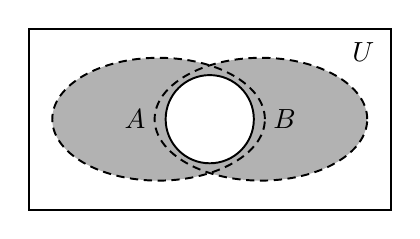
\begin{tikzpicture}[scale=1,line width=0.7pt]
\draw (0,0) rectangle (4.6,2.3);
\fill[black!30] (1.65,1.15) ellipse (1.35 and 0.78);
\fill[black!30] (2.95,1.15) ellipse (1.35 and 0.78);
\fill[white] (2.3,1.15) circle (0.56);
\draw[densely dashed] (1.65,1.15) ellipse (1.35 and 0.78);
\draw[densely dashed] (2.95,1.15) ellipse (1.35 and 0.78);
\draw (2.3,1.15) circle (0.56);
\node at (1.35,1.15) {$A$};
\node at (3.25,1.15) {$B$};
\node at (4.25,2.0) {$U$};
\end{tikzpicture}
\end{center}

\keepwithprev
A. $(-2,1)$\qquad B. $[-1,0]\cup[1,2)$\qquad C. $(-2,-1)\cup[0,1]$\qquad D. $[0,1]$

\ifanswer
\solbegin
\step{$A=\{x\mid-2<x<0\}$，$B=\{x\mid-1\leqslant x\leqslant1\}$，}
\step{所以 $A\cap B=\{x\mid-1\leqslant x<0\}$，$A\cup B=\{x\mid-2<x\leqslant1\}$，}
\step{则图中阴影部分表示的集合是 $(-2,-1)\cup[0,1]$，故选 $C$.}
\solend
\fi

\item 用反证法证明：“若 $x$、$y\in\R$ 且 $x+y>2$，则 $x$、$y$ 中至少有一个大于 $1$”时，应假设\mbox{（\quad）}% 原卷括号内已印“D”，试卷版按惯例留空

\keepwithprev
A. $x$、$y$ 中至少有一个小于 $1$\qquad B. $x$、$y$ 均小于 $1$

C. $x$、$y$ 中至少有一个小于等于 $1$\qquad D. $x$、$y$ 均小于等于 $1$

\ifanswer
\ans{$D$}
\fi

\item 若关于 $x$ 的不等式 $ax^2+bx+c>0$ 的解集是 $(-1,2)$，则不等式 $\dfrac{3ax-b}{x-3}>0$ 的解集是\mbox{（\quad）}

\keepwithprev
A. $\left(-\infty,-\dfrac13\right)\cup(3,+\infty)$\qquad B. $\left(-\dfrac13,3\right)$

C. $(-\infty,-3)\cup\left(\dfrac13,+\infty\right)$\qquad D. $\left(-3,\dfrac13\right)$

\ifanswer
\solbegin
\step{因为不等式 $ax^2+bx+c>0$ 的解集是 $(-1,2)$，}
\step{所以 $-1$、$2$ 是方程 $ax^2+bx+c=0$ 的两个根，且 $a<0$，}
\step{所以 $\begin{cases}-1+2=-\dfrac ba\\ -1\times2=\dfrac ca\end{cases}\Rightarrow\begin{cases}b=-a\\ c=-2a\end{cases}$，}
\step{所以 $\dfrac{3ax-b}{x-3}>0\Rightarrow\dfrac{3ax+a}{x-3}>0\Leftrightarrow a(3x+1)(x-3)>0$，}
\step{又 $a<0$，所以 $(3x+1)(x-3)<0$，解得 $-\dfrac13<x<3$，}
\step{所以不等式 $\dfrac{3ax-b}{x-3}>0$ 的解集为 $\left(-\dfrac13,3\right)$，故选 $B$.}
\solend
\fi

\end{enumerate}

\bigsec{三、解答题}

\begin{enumerate}
\setcounter{enumi}{16}

\item 解下列不等式组：

（1）$\begin{cases}\dfrac{5-x}{x+3}>0\\ 2x-\lvert x-1\rvert>2\end{cases}$；\qquad（2）$\begin{cases}-x^2+x+6\geqslant0\\ \dfrac{x-2}{x+1}\geqslant0\end{cases}$.

\ansspace*[12]

\ifanswer
\solbegin
\stepm{（1）}{不等式 $\dfrac{5-x}{x+3}>0$ 等价于 $(x-5)(x+3)<0$，所以 $-3<x<5$，}
\step{不等式 $2x-\lvert x-1\rvert>2$ 等价于 $2x-2>\lvert x-1\rvert$，}
\step{所以 $2-2x<x-1<2x-2$，故 $x>1$，}
\step{所以不等式组的解集为 $(1,5)$；}
\stepm{（2）}{不等式组 $\begin{cases}-x^2+x+6\geqslant0\\ \dfrac{x-2}{x+1}\geqslant0\end{cases}$ 可化为 $\begin{cases}x^2-x-6\leqslant0\\ (x-2)(x+1)\geqslant0\\ x+1\neq0\end{cases}$，}
\step{解得 $\begin{cases}-2\leqslant x\leqslant3\\ x\leqslant-1\ \text{或}\ x\geqslant2\\ x\neq-1\end{cases}$，即 $-2\leqslant x<-1$ 或 $2\leqslant x\leqslant3$，}
\step{所以不等式组的解集为 $\{x\mid-2\leqslant x<-1$ 或 $2\leqslant x\leqslant3\}$.}
\solend
\fi

\needvspace{3.2cm}
\item 已知 $A=\{x\mid x^2-2x-3\leqslant0\}$，$B=\{x\mid a-1\leqslant x\leqslant2a+1\}$，$a\in\R$.

（1）若 $A\cap B=B$，求实数 $a$ 的取值范围.

（2）若 $a>b>0$，比较 $\dfrac{a^2-b^2}{a^2+b^2}$ 与 $\dfrac{a-b}{a+b}$ 的大小.

\ansspace*[13]

\ifanswer
\solbegin
\stepm{（1）}{解不等式 $x^2-2x-3\leqslant0$，得 $-1\leqslant x\leqslant3$，}
\step{因为 $A\cap B=B$，所以 $B\subseteq A$，}
\step{当 $B=\varnothing$ 时，则 $a-1>2a+1$，解得 $a<-2$，}
\step{当 $B\neq\varnothing$ 时，要使得 $B\subseteq A$，则满足 $\begin{cases}a-1\leqslant2a+1\\ a-1\geqslant-1\\ 2a+1\leqslant3\end{cases}$，解得 $0\leqslant a\leqslant1$，}
\step{综上，实数 $a$ 的取值范围为 $(-\infty,-2)\cup[0,1]$.}
\stepm{（2）}{因为 $a>b>0$，所以 $a-b>0$，$a+b>0$，$ab>0$，}
\step{所以 $a^2-b^2=(a-b)(a+b)>0$，$a^2+b^2+2ab>a^2+b^2>0$，}
\step{$\dfrac{a^2-b^2}{a^2+b^2}>0$，$\dfrac{a-b}{a+b}>0$，}
\step{$\dfrac{\dfrac{a^2-b^2}{a^2+b^2}}{\dfrac{a-b}{a+b}}=\dfrac{(a-b)(a+b)}{a^2+b^2}\cdot\dfrac{a+b}{a-b}=\dfrac{a^2+b^2+2ab}{a^2+b^2}>1$，}
\step{所以 $\dfrac{a^2-b^2}{a^2+b^2}>\dfrac{a-b}{a+b}$.}
\solend
\fi

\item 汽车在行驶中，由于惯性作用，刹车后还要继续向前滑行一段距离才能停住，我们称这段距离为“刹车距离”. 刹车距离是分析事故的一个重要因素. 在一个限速 $40\mathrm{km}/\mathrm{h}$ 以内的弯道上，甲、乙两辆汽车相向而行，发现情况不对，同时刹车，但还是相碰了，事发后现场测得甲车的刹车距离略超过 $12\mathrm{m}$，乙车的刹车距离略超过 $10\mathrm{m}$，又知甲、乙两种车型的刹车距离 $s(\mathrm{m})$ 与车速 $x(\mathrm{km}/\mathrm{h})$ 之间有如下关系：$s_{\text{甲}}=0.1x+0.01x^2$，$s_{\text{乙}}=0.05x+0.005x^2$. 问：两车相撞的主要责任是谁？

\ansspace*[10]

\ifanswer
\solbegin
\step{由题意列出不等式组 $\begin{cases}0.1x+0.01x^2>12\\ 0.05x+0.005x^2>10\end{cases}$，解得 $\begin{cases}x<-40\ \text{或}\ x>30\\ x<-50\ \text{或}\ x>40\end{cases}$，}
\step{由于 $x>0$，从而可得 $x_{\text{甲}}>30\mathrm{km}/\mathrm{h}$，$x_{\text{乙}}>40\mathrm{km}/\mathrm{h}$.}
\step{经比较得乙车超过限速，应负主要责任.}
\solend
\fi

\item 已知关于 $x$ 的一元二次方程 $x^2+(2m-1)x+m^2-3=0$ 有实数根.

（1）若方程有两个负根，求实数 $m$ 的取值范围；

（2）当 $m=2$ 时，记方程的根为 $x_1$、$x_2$，求代数式 $\lvert x_1-x_2\rvert$ 的值.

\ansspace*[12]

\ifanswer
\solbegin
\stepm{（1）}{由方程有两个负根，得 $\begin{cases}\Delta=(2m-1)^2-4(m^2-3)\geqslant0\\ -(2m-1)<0\\ m^2-3>0\end{cases}$，}
\step{即 $\begin{cases}13-4m\geqslant0\\ 2m-1>0\\ (m-\sqrt3)(m+\sqrt3)>0\end{cases}$，解得 $\sqrt3<m\leqslant\dfrac{13}4$，}
\step{则实数 $m$ 的取值范围为 $\left\{m\left|\sqrt3<m\leqslant\dfrac{13}4\right.\right\}$.}
\stepm{（2）}{当 $m=2$ 时，方程为 $x^2+3x+1=0$，}
\step{此时 $\Delta=3^2-4=5>0$，且 $x_1+x_2=-3$，$x_1x_2=1$，}
\step{则 $\lvert x_1-x_2\rvert=\sqrt{(x_1+x_2)^2-4x_1x_2}=\sqrt{(-3)^2-4}=\sqrt5$.}
\solend
\fi

\item 已知不等式 $\lvert2x-a\rvert\leqslant b$ 的解集为 $A$，不等式 $mx^2-mx-1<0$ 的解集为 $B$.

（1）若 $a=1$，$b=2$，求 $A$.

（2）若 $A=[-1,3]$，求实数 $a$、$b$ 的取值；

（3）若 $B=\R$，求实数 $m$ 的取值范围.

\ansspace*[12]

\ifanswer
\solbegin
\stepm{（1）}{因为 $a=1$，$b=2$，所以不等式 $\lvert2x-a\rvert\leqslant b$ 等价于 $\lvert2x-1\rvert\leqslant2$，}
\step{所以 $-2\leqslant2x-1\leqslant2$，故 $-\dfrac12\leqslant x\leqslant\dfrac32$，所以 $A=\left[-\dfrac12,\dfrac32\right]$；}
\stepm{（2）}{当 $b>0$ 时，不等式 $\lvert2x-a\rvert\leqslant b$ 可化为 $-b\leqslant2x-a\leqslant b$，}
\step{所以 $\dfrac{a-b}2\leqslant x\leqslant\dfrac{a+b}2$，由 $A=[-1,3]$，得 $\dfrac{a-b}2=-1$，$\dfrac{a+b}2=3$；}
\step{当 $b=0$ 时，不等式 $\lvert2x-a\rvert\leqslant b$ 的解集为 $\left\{\dfrac a2\right\}$，不满足要求，}
\step{当 $b<0$ 时，不等式 $\lvert2x-a\rvert\leqslant b$ 的解集为 $\varnothing$，不满足要求，}
\step{所以 $a=2$，$b=4$；}
\stepm{（3）}{由已知不等式 $mx^2-mx-1<0$ 的解集为 $\R$，}
\step{得 $\begin{cases}m<0\\ m^2+4m<0\end{cases}$ 或 $m=0$，解得 $-4<m<0$ 或 $m=0$，}
\step{所以实数 $m$ 的取值范围为 $(-4,0]$.}
\solend
\fi

\end{enumerate}

\end{document}
"
% 紧凑版：xelatex "\def\iscompact{1}% 高一97_浦东中学_10月月考.tex
%   —— 高一上数学“2026-2027 年浦东中学高一上 10 月月考”（讲评版）
% 试卷版：xelatex 高一97_浦东中学_10月月考.tex
% 答案版：xelatex "\def\isanswer{1}\input{高一97_浦东中学_10月月考.tex}"
% 紧凑版：xelatex "\def\iscompact{1}\input{高一97_浦东中学_10月月考.tex}"
%
% 原始材料：微信公众号“魔都数学加油站”文章，连载“27学年高一97”；
% 原文标题“27学年高一97——2026-2027年上海市浦东中学高一上10月月考”；
% 原文链接：https://mp.weixin.qq.com/s/2uW3LikOX3B07IWw7LkF_g。
% 正文为 8 张 PNG 页（`原图/高一97_浦东中学_10月月考/01..08.png`）：04、08 为
% 2560×3620，其余为 4762×6735，按页序读取。
%
% 篇幅与题号：原卷自第 3 题起编号（第 1、2 题不在原文内）。填空题 3—12（10 题）、
% 选择题 13—16（4 题）、解答题 17—21（5 题），共 19 题。
%
% 讲评版：第 15 题无【解析】、答案“D”直接印在题干括号内，本稿试卷版按惯例留空、
% 答案版提 \ans{}；其余 18 题印【解析】，其中第 13、14、16 题的答案在解析末句
% “故选 $B$／$C$／$B$”。
%
% 副标题：原卷未印副标题。本稿按内容标作“集合与常用逻辑用语、不等式”。
%
% 插图：第 14 题题干右侧有一幅韦恩图（全集 $U$ 的矩形内两个相交椭圆 $A$、$B$，
% 阴影为两椭圆的对称差）。原图该页为 2560×3620 的低分辨率页，直接裁切会糊，
% 故按原图布局用 TikZ 重绘（三版都出）。
%
% 与原卷的排版差异：
%   ① 原卷每题下直接印【答案】/【解析】，本稿按全稿惯例将答案与解析置于答案版；
%   ② 原卷未印副标题，本稿补出；填空横线统一排 \blankline[4.4em]；
%   ③ 原卷数集记号排斜体 $R$，本稿按全稿惯例改用 $\R$；
%   ④ 第 14 题的韦恩图原为行内右侧小图，本稿改为居中单列；
%   ⑤ 解答题按惯例加 \ansspace；选择题括号排 \mbox{（\quad）}。
%
% 行数核对：逐题数 \step/\stepm 条数，合计 85 条（Q3：2；Q4：2；Q5：2；Q6：2；
% Q7：2；Q8：4；Q9：4；Q10：5；Q11：10；Q12：3；Q13：4；Q14：3；Q15：0；
% Q16：6；Q17：7；Q18：10；Q19：3；Q20：6；Q21：10）。第 15 题无解析，
% 不计入 \step 账。原卷解析的换行按语意合并，未逐行强拆。
%
\documentclass[a4paper,11pt]{article}
\usepackage{common}

\begin{document}

\examtitlest[2]{2026--2027 年浦东中学高一上 10 月月考}{集合与常用逻辑用语、不等式}

\bigsec{一、填空题}

\begin{enumerate}
\setcounter{enumi}{2}

\item “$a(a-2)<0$”是“$\dfrac2a>1$”成立的\blankline[4.4em]条件（填充分必要性）.

\ifanswer
\solbegin
\step{“不等式 $a(a-2)<0\Rightarrow0<a<2$，不等式 $\dfrac2a>1\Rightarrow\dfrac{2-a}a>0\Rightarrow0<a<2$，}
\step{两不等式解集相等，所以“$a(a-2)<0$”是“$\dfrac2a>1$”成立的充要条件.}
\solend
\fi

\item 求不等式 $\lvert5-2x\rvert\leqslant3$ 的解集\blankline[4.4em].

\ifanswer
\solbegin
\step{$\lvert5-2x\rvert\leqslant3$ 等价于 $-3\leqslant5-2x\leqslant3$，解得 $1\leqslant x\leqslant4$，}
\step{所以不等式 $\lvert5-2x\rvert\leqslant3$ 的解集为 $\{x\mid1\leqslant x\leqslant4\}$.}
\solend
\fi

\item 求不等式组 $\begin{cases}3x^2+2x-1<0\\ \dfrac1x\geqslant0\end{cases}$ 的解集\blankline[4.4em].

\ifanswer
\solbegin
\step{不等式 $3x^2+2x-1=(3x-1)(x+1)<0$，解得 $-1<x<\dfrac13$，}
\step{由不等式 $\dfrac1x\geqslant0$ 解得 $x>0$，所以不等式组的解集为 $\left(0,\dfrac13\right)$.}
\solend
\fi

\item 满足 $\{1,3\}\subseteq A\subseteq\{0,1,3,5\}$ 的所有集合 $A$ 的全部元素之和为\blankline[4.4em].

\ifanswer
\solbegin
\step{符合条件的集合 $A$ 有以下几个，$A_1=\{0,1,3\}$，$A_2=\{1,3,5\}$，$A_3=\{0,1,3,5\}$，}
\step{所以所有集合 $A$ 的全部元素之和为 $0+1+3+1+3+5+0+1+3+5=22$.}
\solend
\fi

\item 已知集合 $A=\{(x,y)\mid y=-x+1\}$，$B=\{(x,y)\mid y=x^2-1\}$，则 $A\cap B=\blankline[4.4em]$.

\ifanswer
\solbegin
\step{联立 $\begin{cases}y=-x+1\\ y=x^2-1\end{cases}$，解得 $\begin{cases}x=1\\ y=0\end{cases}$ 或 $\begin{cases}x=-2\\ y=3\end{cases}$，}
\step{故 $A\cap B=\{(1,0),(-2,3)\}$.}
\solend
\fi

\item 若 $a$、$b$ 是方程 $x^2+2x-3=0$ 的两个实数根，则 $a^2-2b=\blankline[4.4em]$.

\ifanswer
\solbegin
\step{$a$、$b$ 是方程 $x^2+2x-3=0$ 的两个实数根，}
\step{所以 $a^2+2a-3=0$，故 $a^2=3-2a$，}
\step{由韦达定理得 $a+b=-2$，所以 $b=-2-a$，}
\step{所以 $a^2-2b=3-2a-2b=3-2a+4+2a=7$.}
\solend
\fi

\item 设 $a$、$b$ 为实数，若不等式 $x^2-ax-b<0$ 的解集为 $(2,8)$，则 $bx^2-ax-1>0$ 的解集为\blankline[4.4em].

\ifanswer
\solbegin
\step{因为不等式 $x^2-ax-b<0$ 的解集为 $(2,8)$，所以 $\begin{cases}2+8=a\\ 2\times8=-b\end{cases}$，}
\step{所以 $a=10$，$b=-16$，所以 $bx^2-ax-1>0$ 可化为 $-16x^2-10x-1>0$，}
\step{所以 $16x^2+10x+1<0$，}
\step{所以所求不等式的解集为 $\left(-\dfrac12,-\dfrac18\right)$.}
\solend
\fi

\item 若集合 $A=\{x\mid x^2+3x-4=0\}$，$B=\{x\mid ax-1=0\}$，若 $A\cap B=B$，则实数 $a$ 的取值组成的集合是\blankline[4.4em].

\ifanswer
\solbegin
\step{集合 $A=\{x\mid x^2+3x-4=0\}=\{-4,1\}$，$B=\{x\mid ax-1=0\}$，}
\step{因为 $A\cap B=B$，所以 $B\subseteq A$，}
\step{当 $a=0$ 时，$B=\varnothing$，$B\subseteq A$ 成立；}
\step{当 $a\neq0$ 时，$B=\left\{\dfrac1a\right\}$，由 $B\subseteq A$，得 $\dfrac1a=-4$ 或 $\dfrac1a=1$，解得 $a=-\dfrac14$ 或 $a=1$，}
\step{所以实数 $a$ 的值为 $-\dfrac14$ 或 $0$ 或 $1$，实数 $a$ 的取值组成的集合是 $\left\{-\dfrac14,0,1\right\}$.}
\solend
\fi

\item 关于 $x$ 的不等式 $ax^2+(1-2a^2)x-2a<0$ 的解集中恰有 $3$ 个正整数解，则 $a$ 的取值范围为\blankline[4.4em].

\ifanswer
\solbegin
\step{①当 $a=0$ 时，不等式化为 $x<0$，则解集中有无数个整数，不满足题意；}
\step{当 $a\neq0$ 时，不等式 $ax^2+(1-2a^2)x-2a<0$ 的解集中恰有 $3$ 个正整数解，}
\step{即为不等式 $(ax+1)(x-2a)<0$ 的解集中恰有 $3$ 个正整数解，}
\step{②当 $a<0$ 时，不等式 $(ax+1)(x-2a)<0$ 的解集中有无数个正整数，}
\step{不满足题意，}
\step{③当 $a>0$ 时，$-\dfrac1a<0,2a>0$，所以 $-\dfrac1a<2a$，}
\step{所以不等式的解集为 $\left\{x\left|-\dfrac1a<x<2a\right.\right\}$，}
\step{由解集得 $0$ 一定属于此集合，则由不等式的解集中恰有 $3$ 个正整数，}
\step{则这 $3$ 个正整数一定为 $1$，$2$，$3$，则 $3<2a\leqslant4$，解得 $\dfrac32<a\leqslant2$，}
\step{所以 $a$ 的取值范围是 $\left\{a\left|\dfrac32<a\leqslant2\right.\right\}$.}
\solend
\fi

\item 设 $x\in\R$，$[x]$ 表示不大于 $x$ 的最大整数，如 $[\pi]=3$，$[-1.2]=-2$，$\left[\dfrac12\right]=0$，则使 $[\lvert x-1\rvert]=3$ 成立的 $x$ 的取值范围\blankline[4.4em].

\ifanswer
\solbegin
\step{由题意 $[\lvert x-1\rvert]=3$，则 $3\leqslant\lvert x-1\rvert<4$，所以 $3\leqslant x-1<4$ 或 $-4\leqslant x-1<-3$，}
\step{解得 $4\leqslant x<5$ 或 $-3<x\leqslant-2$，}
\step{所以使 $[\lvert x-1\rvert]=3$ 成立的 $x$ 的取值范围是 $(-3,-2]\cup[4,5)$.}
\solend
\fi

\end{enumerate}

\bigsec{二、选择题}

\begin{enumerate}
\setcounter{enumi}{12}

\item 若 $a\in\R$，则“$a^2>a$”是“$a>1$”的\mbox{（\quad）}

\keepwithprev
A. 充分非必要条件\qquad B. 必要非充分条件

C. 充要条件\qquad D. 既非充分又非必要条件

\ifanswer
\solbegin
\step{已知 $a^2>a$，则 $a(a-1)>0$，即 $a<0$ 或 $a>1$，}
\step{由“$a<0$ 或 $a>1$”不能推出“$a>1$”；}
\step{由“$a>1$”可以推出“$a<0$ 或 $a>1$”，即“$a>1$”可以推出“$a^2>a$”；}
\step{所以“$a^2>a$”是“$a>1$”的必要非充分条件. 故选 $B$.}
\solend
\fi

\item 已知全集 $U=\R$，集合 $A=\{x\mid x(x+2)<0\}$，$B=\{x\mid\lvert x\rvert\leqslant1\}$，则图中阴影部分表示的集合是\mbox{（\quad）}

\begin{center}
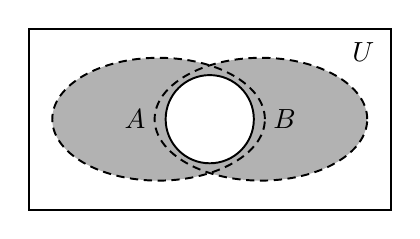
\begin{tikzpicture}[scale=1,line width=0.7pt]
\draw (0,0) rectangle (4.6,2.3);
\fill[black!30] (1.65,1.15) ellipse (1.35 and 0.78);
\fill[black!30] (2.95,1.15) ellipse (1.35 and 0.78);
\fill[white] (2.3,1.15) circle (0.56);
\draw[densely dashed] (1.65,1.15) ellipse (1.35 and 0.78);
\draw[densely dashed] (2.95,1.15) ellipse (1.35 and 0.78);
\draw (2.3,1.15) circle (0.56);
\node at (1.35,1.15) {$A$};
\node at (3.25,1.15) {$B$};
\node at (4.25,2.0) {$U$};
\end{tikzpicture}
\end{center}

\keepwithprev
A. $(-2,1)$\qquad B. $[-1,0]\cup[1,2)$\qquad C. $(-2,-1)\cup[0,1]$\qquad D. $[0,1]$

\ifanswer
\solbegin
\step{$A=\{x\mid-2<x<0\}$，$B=\{x\mid-1\leqslant x\leqslant1\}$，}
\step{所以 $A\cap B=\{x\mid-1\leqslant x<0\}$，$A\cup B=\{x\mid-2<x\leqslant1\}$，}
\step{则图中阴影部分表示的集合是 $(-2,-1)\cup[0,1]$，故选 $C$.}
\solend
\fi

\item 用反证法证明：“若 $x$、$y\in\R$ 且 $x+y>2$，则 $x$、$y$ 中至少有一个大于 $1$”时，应假设\mbox{（\quad）}% 原卷括号内已印“D”，试卷版按惯例留空

\keepwithprev
A. $x$、$y$ 中至少有一个小于 $1$\qquad B. $x$、$y$ 均小于 $1$

C. $x$、$y$ 中至少有一个小于等于 $1$\qquad D. $x$、$y$ 均小于等于 $1$

\ifanswer
\ans{$D$}
\fi

\item 若关于 $x$ 的不等式 $ax^2+bx+c>0$ 的解集是 $(-1,2)$，则不等式 $\dfrac{3ax-b}{x-3}>0$ 的解集是\mbox{（\quad）}

\keepwithprev
A. $\left(-\infty,-\dfrac13\right)\cup(3,+\infty)$\qquad B. $\left(-\dfrac13,3\right)$

C. $(-\infty,-3)\cup\left(\dfrac13,+\infty\right)$\qquad D. $\left(-3,\dfrac13\right)$

\ifanswer
\solbegin
\step{因为不等式 $ax^2+bx+c>0$ 的解集是 $(-1,2)$，}
\step{所以 $-1$、$2$ 是方程 $ax^2+bx+c=0$ 的两个根，且 $a<0$，}
\step{所以 $\begin{cases}-1+2=-\dfrac ba\\ -1\times2=\dfrac ca\end{cases}\Rightarrow\begin{cases}b=-a\\ c=-2a\end{cases}$，}
\step{所以 $\dfrac{3ax-b}{x-3}>0\Rightarrow\dfrac{3ax+a}{x-3}>0\Leftrightarrow a(3x+1)(x-3)>0$，}
\step{又 $a<0$，所以 $(3x+1)(x-3)<0$，解得 $-\dfrac13<x<3$，}
\step{所以不等式 $\dfrac{3ax-b}{x-3}>0$ 的解集为 $\left(-\dfrac13,3\right)$，故选 $B$.}
\solend
\fi

\end{enumerate}

\bigsec{三、解答题}

\begin{enumerate}
\setcounter{enumi}{16}

\item 解下列不等式组：

（1）$\begin{cases}\dfrac{5-x}{x+3}>0\\ 2x-\lvert x-1\rvert>2\end{cases}$；\qquad（2）$\begin{cases}-x^2+x+6\geqslant0\\ \dfrac{x-2}{x+1}\geqslant0\end{cases}$.

\ansspace*[12]

\ifanswer
\solbegin
\stepm{（1）}{不等式 $\dfrac{5-x}{x+3}>0$ 等价于 $(x-5)(x+3)<0$，所以 $-3<x<5$，}
\step{不等式 $2x-\lvert x-1\rvert>2$ 等价于 $2x-2>\lvert x-1\rvert$，}
\step{所以 $2-2x<x-1<2x-2$，故 $x>1$，}
\step{所以不等式组的解集为 $(1,5)$；}
\stepm{（2）}{不等式组 $\begin{cases}-x^2+x+6\geqslant0\\ \dfrac{x-2}{x+1}\geqslant0\end{cases}$ 可化为 $\begin{cases}x^2-x-6\leqslant0\\ (x-2)(x+1)\geqslant0\\ x+1\neq0\end{cases}$，}
\step{解得 $\begin{cases}-2\leqslant x\leqslant3\\ x\leqslant-1\ \text{或}\ x\geqslant2\\ x\neq-1\end{cases}$，即 $-2\leqslant x<-1$ 或 $2\leqslant x\leqslant3$，}
\step{所以不等式组的解集为 $\{x\mid-2\leqslant x<-1$ 或 $2\leqslant x\leqslant3\}$.}
\solend
\fi

\needvspace{3.2cm}
\item 已知 $A=\{x\mid x^2-2x-3\leqslant0\}$，$B=\{x\mid a-1\leqslant x\leqslant2a+1\}$，$a\in\R$.

（1）若 $A\cap B=B$，求实数 $a$ 的取值范围.

（2）若 $a>b>0$，比较 $\dfrac{a^2-b^2}{a^2+b^2}$ 与 $\dfrac{a-b}{a+b}$ 的大小.

\ansspace*[13]

\ifanswer
\solbegin
\stepm{（1）}{解不等式 $x^2-2x-3\leqslant0$，得 $-1\leqslant x\leqslant3$，}
\step{因为 $A\cap B=B$，所以 $B\subseteq A$，}
\step{当 $B=\varnothing$ 时，则 $a-1>2a+1$，解得 $a<-2$，}
\step{当 $B\neq\varnothing$ 时，要使得 $B\subseteq A$，则满足 $\begin{cases}a-1\leqslant2a+1\\ a-1\geqslant-1\\ 2a+1\leqslant3\end{cases}$，解得 $0\leqslant a\leqslant1$，}
\step{综上，实数 $a$ 的取值范围为 $(-\infty,-2)\cup[0,1]$.}
\stepm{（2）}{因为 $a>b>0$，所以 $a-b>0$，$a+b>0$，$ab>0$，}
\step{所以 $a^2-b^2=(a-b)(a+b)>0$，$a^2+b^2+2ab>a^2+b^2>0$，}
\step{$\dfrac{a^2-b^2}{a^2+b^2}>0$，$\dfrac{a-b}{a+b}>0$，}
\step{$\dfrac{\dfrac{a^2-b^2}{a^2+b^2}}{\dfrac{a-b}{a+b}}=\dfrac{(a-b)(a+b)}{a^2+b^2}\cdot\dfrac{a+b}{a-b}=\dfrac{a^2+b^2+2ab}{a^2+b^2}>1$，}
\step{所以 $\dfrac{a^2-b^2}{a^2+b^2}>\dfrac{a-b}{a+b}$.}
\solend
\fi

\item 汽车在行驶中，由于惯性作用，刹车后还要继续向前滑行一段距离才能停住，我们称这段距离为“刹车距离”. 刹车距离是分析事故的一个重要因素. 在一个限速 $40\mathrm{km}/\mathrm{h}$ 以内的弯道上，甲、乙两辆汽车相向而行，发现情况不对，同时刹车，但还是相碰了，事发后现场测得甲车的刹车距离略超过 $12\mathrm{m}$，乙车的刹车距离略超过 $10\mathrm{m}$，又知甲、乙两种车型的刹车距离 $s(\mathrm{m})$ 与车速 $x(\mathrm{km}/\mathrm{h})$ 之间有如下关系：$s_{\text{甲}}=0.1x+0.01x^2$，$s_{\text{乙}}=0.05x+0.005x^2$. 问：两车相撞的主要责任是谁？

\ansspace*[10]

\ifanswer
\solbegin
\step{由题意列出不等式组 $\begin{cases}0.1x+0.01x^2>12\\ 0.05x+0.005x^2>10\end{cases}$，解得 $\begin{cases}x<-40\ \text{或}\ x>30\\ x<-50\ \text{或}\ x>40\end{cases}$，}
\step{由于 $x>0$，从而可得 $x_{\text{甲}}>30\mathrm{km}/\mathrm{h}$，$x_{\text{乙}}>40\mathrm{km}/\mathrm{h}$.}
\step{经比较得乙车超过限速，应负主要责任.}
\solend
\fi

\item 已知关于 $x$ 的一元二次方程 $x^2+(2m-1)x+m^2-3=0$ 有实数根.

（1）若方程有两个负根，求实数 $m$ 的取值范围；

（2）当 $m=2$ 时，记方程的根为 $x_1$、$x_2$，求代数式 $\lvert x_1-x_2\rvert$ 的值.

\ansspace*[12]

\ifanswer
\solbegin
\stepm{（1）}{由方程有两个负根，得 $\begin{cases}\Delta=(2m-1)^2-4(m^2-3)\geqslant0\\ -(2m-1)<0\\ m^2-3>0\end{cases}$，}
\step{即 $\begin{cases}13-4m\geqslant0\\ 2m-1>0\\ (m-\sqrt3)(m+\sqrt3)>0\end{cases}$，解得 $\sqrt3<m\leqslant\dfrac{13}4$，}
\step{则实数 $m$ 的取值范围为 $\left\{m\left|\sqrt3<m\leqslant\dfrac{13}4\right.\right\}$.}
\stepm{（2）}{当 $m=2$ 时，方程为 $x^2+3x+1=0$，}
\step{此时 $\Delta=3^2-4=5>0$，且 $x_1+x_2=-3$，$x_1x_2=1$，}
\step{则 $\lvert x_1-x_2\rvert=\sqrt{(x_1+x_2)^2-4x_1x_2}=\sqrt{(-3)^2-4}=\sqrt5$.}
\solend
\fi

\item 已知不等式 $\lvert2x-a\rvert\leqslant b$ 的解集为 $A$，不等式 $mx^2-mx-1<0$ 的解集为 $B$.

（1）若 $a=1$，$b=2$，求 $A$.

（2）若 $A=[-1,3]$，求实数 $a$、$b$ 的取值；

（3）若 $B=\R$，求实数 $m$ 的取值范围.

\ansspace*[12]

\ifanswer
\solbegin
\stepm{（1）}{因为 $a=1$，$b=2$，所以不等式 $\lvert2x-a\rvert\leqslant b$ 等价于 $\lvert2x-1\rvert\leqslant2$，}
\step{所以 $-2\leqslant2x-1\leqslant2$，故 $-\dfrac12\leqslant x\leqslant\dfrac32$，所以 $A=\left[-\dfrac12,\dfrac32\right]$；}
\stepm{（2）}{当 $b>0$ 时，不等式 $\lvert2x-a\rvert\leqslant b$ 可化为 $-b\leqslant2x-a\leqslant b$，}
\step{所以 $\dfrac{a-b}2\leqslant x\leqslant\dfrac{a+b}2$，由 $A=[-1,3]$，得 $\dfrac{a-b}2=-1$，$\dfrac{a+b}2=3$；}
\step{当 $b=0$ 时，不等式 $\lvert2x-a\rvert\leqslant b$ 的解集为 $\left\{\dfrac a2\right\}$，不满足要求，}
\step{当 $b<0$ 时，不等式 $\lvert2x-a\rvert\leqslant b$ 的解集为 $\varnothing$，不满足要求，}
\step{所以 $a=2$，$b=4$；}
\stepm{（3）}{由已知不等式 $mx^2-mx-1<0$ 的解集为 $\R$，}
\step{得 $\begin{cases}m<0\\ m^2+4m<0\end{cases}$ 或 $m=0$，解得 $-4<m<0$ 或 $m=0$，}
\step{所以实数 $m$ 的取值范围为 $(-4,0]$.}
\solend
\fi

\end{enumerate}

\end{document}
"
%
% 原始材料：微信公众号“魔都数学加油站”文章，连载“27学年高一97”；
% 原文标题“27学年高一97——2026-2027年上海市浦东中学高一上10月月考”；
% 原文链接：https://mp.weixin.qq.com/s/2uW3LikOX3B07IWw7LkF_g。
% 正文为 8 张 PNG 页（`原图/高一97_浦东中学_10月月考/01..08.png`）：04、08 为
% 2560×3620，其余为 4762×6735，按页序读取。
%
% 篇幅与题号：原卷自第 3 题起编号（第 1、2 题不在原文内）。填空题 3—12（10 题）、
% 选择题 13—16（4 题）、解答题 17—21（5 题），共 19 题。
%
% 讲评版：第 15 题无【解析】、答案“D”直接印在题干括号内，本稿试卷版按惯例留空、
% 答案版提 \ans{}；其余 18 题印【解析】，其中第 13、14、16 题的答案在解析末句
% “故选 $B$／$C$／$B$”。
%
% 副标题：原卷未印副标题。本稿按内容标作“集合与常用逻辑用语、不等式”。
%
% 插图：第 14 题题干右侧有一幅韦恩图（全集 $U$ 的矩形内两个相交椭圆 $A$、$B$，
% 阴影为两椭圆的对称差）。原图该页为 2560×3620 的低分辨率页，直接裁切会糊，
% 故按原图布局用 TikZ 重绘（三版都出）。
%
% 与原卷的排版差异：
%   ① 原卷每题下直接印【答案】/【解析】，本稿按全稿惯例将答案与解析置于答案版；
%   ② 原卷未印副标题，本稿补出；填空横线统一排 \blankline[4.4em]；
%   ③ 原卷数集记号排斜体 $R$，本稿按全稿惯例改用 $\R$；
%   ④ 第 14 题的韦恩图原为行内右侧小图，本稿改为居中单列；
%   ⑤ 解答题按惯例加 \ansspace；选择题括号排 \mbox{（\quad）}。
%
% 行数核对：逐题数 \step/\stepm 条数，合计 85 条（Q3：2；Q4：2；Q5：2；Q6：2；
% Q7：2；Q8：4；Q9：4；Q10：5；Q11：10；Q12：3；Q13：4；Q14：3；Q15：0；
% Q16：6；Q17：7；Q18：10；Q19：3；Q20：6；Q21：10）。第 15 题无解析，
% 不计入 \step 账。原卷解析的换行按语意合并，未逐行强拆。
%
\documentclass[a4paper,11pt]{article}
\usepackage{common}

\begin{document}

\examtitlest[2]{2026--2027 年浦东中学高一上 10 月月考}{集合与常用逻辑用语、不等式}

\bigsec{一、填空题}

\begin{enumerate}
\setcounter{enumi}{2}

\item “$a(a-2)<0$”是“$\dfrac2a>1$”成立的\blankline[4.4em]条件（填充分必要性）.

\ifanswer
\solbegin
\step{“不等式 $a(a-2)<0\Rightarrow0<a<2$，不等式 $\dfrac2a>1\Rightarrow\dfrac{2-a}a>0\Rightarrow0<a<2$，}
\step{两不等式解集相等，所以“$a(a-2)<0$”是“$\dfrac2a>1$”成立的充要条件.}
\solend
\fi

\item 求不等式 $\lvert5-2x\rvert\leqslant3$ 的解集\blankline[4.4em].

\ifanswer
\solbegin
\step{$\lvert5-2x\rvert\leqslant3$ 等价于 $-3\leqslant5-2x\leqslant3$，解得 $1\leqslant x\leqslant4$，}
\step{所以不等式 $\lvert5-2x\rvert\leqslant3$ 的解集为 $\{x\mid1\leqslant x\leqslant4\}$.}
\solend
\fi

\item 求不等式组 $\begin{cases}3x^2+2x-1<0\\ \dfrac1x\geqslant0\end{cases}$ 的解集\blankline[4.4em].

\ifanswer
\solbegin
\step{不等式 $3x^2+2x-1=(3x-1)(x+1)<0$，解得 $-1<x<\dfrac13$，}
\step{由不等式 $\dfrac1x\geqslant0$ 解得 $x>0$，所以不等式组的解集为 $\left(0,\dfrac13\right)$.}
\solend
\fi

\item 满足 $\{1,3\}\subseteq A\subseteq\{0,1,3,5\}$ 的所有集合 $A$ 的全部元素之和为\blankline[4.4em].

\ifanswer
\solbegin
\step{符合条件的集合 $A$ 有以下几个，$A_1=\{0,1,3\}$，$A_2=\{1,3,5\}$，$A_3=\{0,1,3,5\}$，}
\step{所以所有集合 $A$ 的全部元素之和为 $0+1+3+1+3+5+0+1+3+5=22$.}
\solend
\fi

\item 已知集合 $A=\{(x,y)\mid y=-x+1\}$，$B=\{(x,y)\mid y=x^2-1\}$，则 $A\cap B=\blankline[4.4em]$.

\ifanswer
\solbegin
\step{联立 $\begin{cases}y=-x+1\\ y=x^2-1\end{cases}$，解得 $\begin{cases}x=1\\ y=0\end{cases}$ 或 $\begin{cases}x=-2\\ y=3\end{cases}$，}
\step{故 $A\cap B=\{(1,0),(-2,3)\}$.}
\solend
\fi

\item 若 $a$、$b$ 是方程 $x^2+2x-3=0$ 的两个实数根，则 $a^2-2b=\blankline[4.4em]$.

\ifanswer
\solbegin
\step{$a$、$b$ 是方程 $x^2+2x-3=0$ 的两个实数根，}
\step{所以 $a^2+2a-3=0$，故 $a^2=3-2a$，}
\step{由韦达定理得 $a+b=-2$，所以 $b=-2-a$，}
\step{所以 $a^2-2b=3-2a-2b=3-2a+4+2a=7$.}
\solend
\fi

\item 设 $a$、$b$ 为实数，若不等式 $x^2-ax-b<0$ 的解集为 $(2,8)$，则 $bx^2-ax-1>0$ 的解集为\blankline[4.4em].

\ifanswer
\solbegin
\step{因为不等式 $x^2-ax-b<0$ 的解集为 $(2,8)$，所以 $\begin{cases}2+8=a\\ 2\times8=-b\end{cases}$，}
\step{所以 $a=10$，$b=-16$，所以 $bx^2-ax-1>0$ 可化为 $-16x^2-10x-1>0$，}
\step{所以 $16x^2+10x+1<0$，}
\step{所以所求不等式的解集为 $\left(-\dfrac12,-\dfrac18\right)$.}
\solend
\fi

\item 若集合 $A=\{x\mid x^2+3x-4=0\}$，$B=\{x\mid ax-1=0\}$，若 $A\cap B=B$，则实数 $a$ 的取值组成的集合是\blankline[4.4em].

\ifanswer
\solbegin
\step{集合 $A=\{x\mid x^2+3x-4=0\}=\{-4,1\}$，$B=\{x\mid ax-1=0\}$，}
\step{因为 $A\cap B=B$，所以 $B\subseteq A$，}
\step{当 $a=0$ 时，$B=\varnothing$，$B\subseteq A$ 成立；}
\step{当 $a\neq0$ 时，$B=\left\{\dfrac1a\right\}$，由 $B\subseteq A$，得 $\dfrac1a=-4$ 或 $\dfrac1a=1$，解得 $a=-\dfrac14$ 或 $a=1$，}
\step{所以实数 $a$ 的值为 $-\dfrac14$ 或 $0$ 或 $1$，实数 $a$ 的取值组成的集合是 $\left\{-\dfrac14,0,1\right\}$.}
\solend
\fi

\item 关于 $x$ 的不等式 $ax^2+(1-2a^2)x-2a<0$ 的解集中恰有 $3$ 个正整数解，则 $a$ 的取值范围为\blankline[4.4em].

\ifanswer
\solbegin
\step{①当 $a=0$ 时，不等式化为 $x<0$，则解集中有无数个整数，不满足题意；}
\step{当 $a\neq0$ 时，不等式 $ax^2+(1-2a^2)x-2a<0$ 的解集中恰有 $3$ 个正整数解，}
\step{即为不等式 $(ax+1)(x-2a)<0$ 的解集中恰有 $3$ 个正整数解，}
\step{②当 $a<0$ 时，不等式 $(ax+1)(x-2a)<0$ 的解集中有无数个正整数，}
\step{不满足题意，}
\step{③当 $a>0$ 时，$-\dfrac1a<0,2a>0$，所以 $-\dfrac1a<2a$，}
\step{所以不等式的解集为 $\left\{x\left|-\dfrac1a<x<2a\right.\right\}$，}
\step{由解集得 $0$ 一定属于此集合，则由不等式的解集中恰有 $3$ 个正整数，}
\step{则这 $3$ 个正整数一定为 $1$，$2$，$3$，则 $3<2a\leqslant4$，解得 $\dfrac32<a\leqslant2$，}
\step{所以 $a$ 的取值范围是 $\left\{a\left|\dfrac32<a\leqslant2\right.\right\}$.}
\solend
\fi

\item 设 $x\in\R$，$[x]$ 表示不大于 $x$ 的最大整数，如 $[\pi]=3$，$[-1.2]=-2$，$\left[\dfrac12\right]=0$，则使 $[\lvert x-1\rvert]=3$ 成立的 $x$ 的取值范围\blankline[4.4em].

\ifanswer
\solbegin
\step{由题意 $[\lvert x-1\rvert]=3$，则 $3\leqslant\lvert x-1\rvert<4$，所以 $3\leqslant x-1<4$ 或 $-4\leqslant x-1<-3$，}
\step{解得 $4\leqslant x<5$ 或 $-3<x\leqslant-2$，}
\step{所以使 $[\lvert x-1\rvert]=3$ 成立的 $x$ 的取值范围是 $(-3,-2]\cup[4,5)$.}
\solend
\fi

\end{enumerate}

\bigsec{二、选择题}

\begin{enumerate}
\setcounter{enumi}{12}

\item 若 $a\in\R$，则“$a^2>a$”是“$a>1$”的\mbox{（\quad）}

\keepwithprev
A. 充分非必要条件\qquad B. 必要非充分条件

C. 充要条件\qquad D. 既非充分又非必要条件

\ifanswer
\solbegin
\step{已知 $a^2>a$，则 $a(a-1)>0$，即 $a<0$ 或 $a>1$，}
\step{由“$a<0$ 或 $a>1$”不能推出“$a>1$”；}
\step{由“$a>1$”可以推出“$a<0$ 或 $a>1$”，即“$a>1$”可以推出“$a^2>a$”；}
\step{所以“$a^2>a$”是“$a>1$”的必要非充分条件. 故选 $B$.}
\solend
\fi

\item 已知全集 $U=\R$，集合 $A=\{x\mid x(x+2)<0\}$，$B=\{x\mid\lvert x\rvert\leqslant1\}$，则图中阴影部分表示的集合是\mbox{（\quad）}

\begin{center}
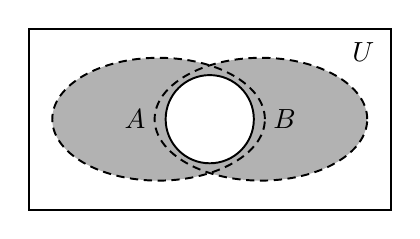
\begin{tikzpicture}[scale=1,line width=0.7pt]
\draw (0,0) rectangle (4.6,2.3);
\fill[black!30] (1.65,1.15) ellipse (1.35 and 0.78);
\fill[black!30] (2.95,1.15) ellipse (1.35 and 0.78);
\fill[white] (2.3,1.15) circle (0.56);
\draw[densely dashed] (1.65,1.15) ellipse (1.35 and 0.78);
\draw[densely dashed] (2.95,1.15) ellipse (1.35 and 0.78);
\draw (2.3,1.15) circle (0.56);
\node at (1.35,1.15) {$A$};
\node at (3.25,1.15) {$B$};
\node at (4.25,2.0) {$U$};
\end{tikzpicture}
\end{center}

\keepwithprev
A. $(-2,1)$\qquad B. $[-1,0]\cup[1,2)$\qquad C. $(-2,-1)\cup[0,1]$\qquad D. $[0,1]$

\ifanswer
\solbegin
\step{$A=\{x\mid-2<x<0\}$，$B=\{x\mid-1\leqslant x\leqslant1\}$，}
\step{所以 $A\cap B=\{x\mid-1\leqslant x<0\}$，$A\cup B=\{x\mid-2<x\leqslant1\}$，}
\step{则图中阴影部分表示的集合是 $(-2,-1)\cup[0,1]$，故选 $C$.}
\solend
\fi

\item 用反证法证明：“若 $x$、$y\in\R$ 且 $x+y>2$，则 $x$、$y$ 中至少有一个大于 $1$”时，应假设\mbox{（\quad）}% 原卷括号内已印“D”，试卷版按惯例留空

\keepwithprev
A. $x$、$y$ 中至少有一个小于 $1$\qquad B. $x$、$y$ 均小于 $1$

C. $x$、$y$ 中至少有一个小于等于 $1$\qquad D. $x$、$y$ 均小于等于 $1$

\ifanswer
\ans{$D$}
\fi

\item 若关于 $x$ 的不等式 $ax^2+bx+c>0$ 的解集是 $(-1,2)$，则不等式 $\dfrac{3ax-b}{x-3}>0$ 的解集是\mbox{（\quad）}

\keepwithprev
A. $\left(-\infty,-\dfrac13\right)\cup(3,+\infty)$\qquad B. $\left(-\dfrac13,3\right)$

C. $(-\infty,-3)\cup\left(\dfrac13,+\infty\right)$\qquad D. $\left(-3,\dfrac13\right)$

\ifanswer
\solbegin
\step{因为不等式 $ax^2+bx+c>0$ 的解集是 $(-1,2)$，}
\step{所以 $-1$、$2$ 是方程 $ax^2+bx+c=0$ 的两个根，且 $a<0$，}
\step{所以 $\begin{cases}-1+2=-\dfrac ba\\ -1\times2=\dfrac ca\end{cases}\Rightarrow\begin{cases}b=-a\\ c=-2a\end{cases}$，}
\step{所以 $\dfrac{3ax-b}{x-3}>0\Rightarrow\dfrac{3ax+a}{x-3}>0\Leftrightarrow a(3x+1)(x-3)>0$，}
\step{又 $a<0$，所以 $(3x+1)(x-3)<0$，解得 $-\dfrac13<x<3$，}
\step{所以不等式 $\dfrac{3ax-b}{x-3}>0$ 的解集为 $\left(-\dfrac13,3\right)$，故选 $B$.}
\solend
\fi

\end{enumerate}

\bigsec{三、解答题}

\begin{enumerate}
\setcounter{enumi}{16}

\item 解下列不等式组：

（1）$\begin{cases}\dfrac{5-x}{x+3}>0\\ 2x-\lvert x-1\rvert>2\end{cases}$；\qquad（2）$\begin{cases}-x^2+x+6\geqslant0\\ \dfrac{x-2}{x+1}\geqslant0\end{cases}$.

\ansspace*[12]

\ifanswer
\solbegin
\stepm{（1）}{不等式 $\dfrac{5-x}{x+3}>0$ 等价于 $(x-5)(x+3)<0$，所以 $-3<x<5$，}
\step{不等式 $2x-\lvert x-1\rvert>2$ 等价于 $2x-2>\lvert x-1\rvert$，}
\step{所以 $2-2x<x-1<2x-2$，故 $x>1$，}
\step{所以不等式组的解集为 $(1,5)$；}
\stepm{（2）}{不等式组 $\begin{cases}-x^2+x+6\geqslant0\\ \dfrac{x-2}{x+1}\geqslant0\end{cases}$ 可化为 $\begin{cases}x^2-x-6\leqslant0\\ (x-2)(x+1)\geqslant0\\ x+1\neq0\end{cases}$，}
\step{解得 $\begin{cases}-2\leqslant x\leqslant3\\ x\leqslant-1\ \text{或}\ x\geqslant2\\ x\neq-1\end{cases}$，即 $-2\leqslant x<-1$ 或 $2\leqslant x\leqslant3$，}
\step{所以不等式组的解集为 $\{x\mid-2\leqslant x<-1$ 或 $2\leqslant x\leqslant3\}$.}
\solend
\fi

\needvspace{3.2cm}
\item 已知 $A=\{x\mid x^2-2x-3\leqslant0\}$，$B=\{x\mid a-1\leqslant x\leqslant2a+1\}$，$a\in\R$.

（1）若 $A\cap B=B$，求实数 $a$ 的取值范围.

（2）若 $a>b>0$，比较 $\dfrac{a^2-b^2}{a^2+b^2}$ 与 $\dfrac{a-b}{a+b}$ 的大小.

\ansspace*[13]

\ifanswer
\solbegin
\stepm{（1）}{解不等式 $x^2-2x-3\leqslant0$，得 $-1\leqslant x\leqslant3$，}
\step{因为 $A\cap B=B$，所以 $B\subseteq A$，}
\step{当 $B=\varnothing$ 时，则 $a-1>2a+1$，解得 $a<-2$，}
\step{当 $B\neq\varnothing$ 时，要使得 $B\subseteq A$，则满足 $\begin{cases}a-1\leqslant2a+1\\ a-1\geqslant-1\\ 2a+1\leqslant3\end{cases}$，解得 $0\leqslant a\leqslant1$，}
\step{综上，实数 $a$ 的取值范围为 $(-\infty,-2)\cup[0,1]$.}
\stepm{（2）}{因为 $a>b>0$，所以 $a-b>0$，$a+b>0$，$ab>0$，}
\step{所以 $a^2-b^2=(a-b)(a+b)>0$，$a^2+b^2+2ab>a^2+b^2>0$，}
\step{$\dfrac{a^2-b^2}{a^2+b^2}>0$，$\dfrac{a-b}{a+b}>0$，}
\step{$\dfrac{\dfrac{a^2-b^2}{a^2+b^2}}{\dfrac{a-b}{a+b}}=\dfrac{(a-b)(a+b)}{a^2+b^2}\cdot\dfrac{a+b}{a-b}=\dfrac{a^2+b^2+2ab}{a^2+b^2}>1$，}
\step{所以 $\dfrac{a^2-b^2}{a^2+b^2}>\dfrac{a-b}{a+b}$.}
\solend
\fi

\item 汽车在行驶中，由于惯性作用，刹车后还要继续向前滑行一段距离才能停住，我们称这段距离为“刹车距离”. 刹车距离是分析事故的一个重要因素. 在一个限速 $40\mathrm{km}/\mathrm{h}$ 以内的弯道上，甲、乙两辆汽车相向而行，发现情况不对，同时刹车，但还是相碰了，事发后现场测得甲车的刹车距离略超过 $12\mathrm{m}$，乙车的刹车距离略超过 $10\mathrm{m}$，又知甲、乙两种车型的刹车距离 $s(\mathrm{m})$ 与车速 $x(\mathrm{km}/\mathrm{h})$ 之间有如下关系：$s_{\text{甲}}=0.1x+0.01x^2$，$s_{\text{乙}}=0.05x+0.005x^2$. 问：两车相撞的主要责任是谁？

\ansspace*[10]

\ifanswer
\solbegin
\step{由题意列出不等式组 $\begin{cases}0.1x+0.01x^2>12\\ 0.05x+0.005x^2>10\end{cases}$，解得 $\begin{cases}x<-40\ \text{或}\ x>30\\ x<-50\ \text{或}\ x>40\end{cases}$，}
\step{由于 $x>0$，从而可得 $x_{\text{甲}}>30\mathrm{km}/\mathrm{h}$，$x_{\text{乙}}>40\mathrm{km}/\mathrm{h}$.}
\step{经比较得乙车超过限速，应负主要责任.}
\solend
\fi

\item 已知关于 $x$ 的一元二次方程 $x^2+(2m-1)x+m^2-3=0$ 有实数根.

（1）若方程有两个负根，求实数 $m$ 的取值范围；

（2）当 $m=2$ 时，记方程的根为 $x_1$、$x_2$，求代数式 $\lvert x_1-x_2\rvert$ 的值.

\ansspace*[12]

\ifanswer
\solbegin
\stepm{（1）}{由方程有两个负根，得 $\begin{cases}\Delta=(2m-1)^2-4(m^2-3)\geqslant0\\ -(2m-1)<0\\ m^2-3>0\end{cases}$，}
\step{即 $\begin{cases}13-4m\geqslant0\\ 2m-1>0\\ (m-\sqrt3)(m+\sqrt3)>0\end{cases}$，解得 $\sqrt3<m\leqslant\dfrac{13}4$，}
\step{则实数 $m$ 的取值范围为 $\left\{m\left|\sqrt3<m\leqslant\dfrac{13}4\right.\right\}$.}
\stepm{（2）}{当 $m=2$ 时，方程为 $x^2+3x+1=0$，}
\step{此时 $\Delta=3^2-4=5>0$，且 $x_1+x_2=-3$，$x_1x_2=1$，}
\step{则 $\lvert x_1-x_2\rvert=\sqrt{(x_1+x_2)^2-4x_1x_2}=\sqrt{(-3)^2-4}=\sqrt5$.}
\solend
\fi

\item 已知不等式 $\lvert2x-a\rvert\leqslant b$ 的解集为 $A$，不等式 $mx^2-mx-1<0$ 的解集为 $B$.

（1）若 $a=1$，$b=2$，求 $A$.

（2）若 $A=[-1,3]$，求实数 $a$、$b$ 的取值；

（3）若 $B=\R$，求实数 $m$ 的取值范围.

\ansspace*[12]

\ifanswer
\solbegin
\stepm{（1）}{因为 $a=1$，$b=2$，所以不等式 $\lvert2x-a\rvert\leqslant b$ 等价于 $\lvert2x-1\rvert\leqslant2$，}
\step{所以 $-2\leqslant2x-1\leqslant2$，故 $-\dfrac12\leqslant x\leqslant\dfrac32$，所以 $A=\left[-\dfrac12,\dfrac32\right]$；}
\stepm{（2）}{当 $b>0$ 时，不等式 $\lvert2x-a\rvert\leqslant b$ 可化为 $-b\leqslant2x-a\leqslant b$，}
\step{所以 $\dfrac{a-b}2\leqslant x\leqslant\dfrac{a+b}2$，由 $A=[-1,3]$，得 $\dfrac{a-b}2=-1$，$\dfrac{a+b}2=3$；}
\step{当 $b=0$ 时，不等式 $\lvert2x-a\rvert\leqslant b$ 的解集为 $\left\{\dfrac a2\right\}$，不满足要求，}
\step{当 $b<0$ 时，不等式 $\lvert2x-a\rvert\leqslant b$ 的解集为 $\varnothing$，不满足要求，}
\step{所以 $a=2$，$b=4$；}
\stepm{（3）}{由已知不等式 $mx^2-mx-1<0$ 的解集为 $\R$，}
\step{得 $\begin{cases}m<0\\ m^2+4m<0\end{cases}$ 或 $m=0$，解得 $-4<m<0$ 或 $m=0$，}
\step{所以实数 $m$ 的取值范围为 $(-4,0]$.}
\solend
\fi

\end{enumerate}

\end{document}
"
%
% 原始材料：微信公众号“魔都数学加油站”文章，连载“27学年高一97”；
% 原文标题“27学年高一97——2026-2027年上海市浦东中学高一上10月月考”；
% 原文链接：https://mp.weixin.qq.com/s/2uW3LikOX3B07IWw7LkF_g。
% 正文为 8 张 PNG 页（`原图/高一97_浦东中学_10月月考/01..08.png`）：04、08 为
% 2560×3620，其余为 4762×6735，按页序读取。
%
% 篇幅与题号：原卷自第 3 题起编号（第 1、2 题不在原文内）。填空题 3—12（10 题）、
% 选择题 13—16（4 题）、解答题 17—21（5 题），共 19 题。
%
% 讲评版：第 15 题无【解析】、答案“D”直接印在题干括号内，本稿试卷版按惯例留空、
% 答案版提 \ans{}；其余 18 题印【解析】，其中第 13、14、16 题的答案在解析末句
% “故选 $B$／$C$／$B$”。
%
% 副标题：原卷未印副标题。本稿按内容标作“集合与常用逻辑用语、不等式”。
%
% 插图：第 14 题题干右侧有一幅韦恩图（全集 $U$ 的矩形内两个相交椭圆 $A$、$B$，
% 阴影为两椭圆的对称差）。原图该页为 2560×3620 的低分辨率页，直接裁切会糊，
% 故按原图布局用 TikZ 重绘（三版都出）。
%
% 与原卷的排版差异：
%   ① 原卷每题下直接印【答案】/【解析】，本稿按全稿惯例将答案与解析置于答案版；
%   ② 原卷未印副标题，本稿补出；填空横线统一排 \blankline[4.4em]；
%   ③ 原卷数集记号排斜体 $R$，本稿按全稿惯例改用 $\R$；
%   ④ 第 14 题的韦恩图原为行内右侧小图，本稿改为居中单列；
%   ⑤ 解答题按惯例加 \ansspace；选择题括号排 \mbox{（\quad）}。
%
% 行数核对：逐题数 \step/\stepm 条数，合计 85 条（Q3：2；Q4：2；Q5：2；Q6：2；
% Q7：2；Q8：4；Q9：4；Q10：5；Q11：10；Q12：3；Q13：4；Q14：3；Q15：0；
% Q16：6；Q17：7；Q18：10；Q19：3；Q20：6；Q21：10）。第 15 题无解析，
% 不计入 \step 账。原卷解析的换行按语意合并，未逐行强拆。
%
\documentclass[a4paper,11pt]{article}
\usepackage{common}

\begin{document}

\examtitlest[2]{2026--2027 年浦东中学高一上 10 月月考}{集合与常用逻辑用语、不等式}

\bigsec{一、填空题}

\begin{enumerate}
\setcounter{enumi}{2}

\item “$a(a-2)<0$”是“$\dfrac2a>1$”成立的\blankline[4.4em]条件（填充分必要性）.

\ifanswer
\solbegin
\step{“不等式 $a(a-2)<0\Rightarrow0<a<2$，不等式 $\dfrac2a>1\Rightarrow\dfrac{2-a}a>0\Rightarrow0<a<2$，}
\step{两不等式解集相等，所以“$a(a-2)<0$”是“$\dfrac2a>1$”成立的充要条件.}
\solend
\fi

\item 求不等式 $\lvert5-2x\rvert\leqslant3$ 的解集\blankline[4.4em].

\ifanswer
\solbegin
\step{$\lvert5-2x\rvert\leqslant3$ 等价于 $-3\leqslant5-2x\leqslant3$，解得 $1\leqslant x\leqslant4$，}
\step{所以不等式 $\lvert5-2x\rvert\leqslant3$ 的解集为 $\{x\mid1\leqslant x\leqslant4\}$.}
\solend
\fi

\item 求不等式组 $\begin{cases}3x^2+2x-1<0\\ \dfrac1x\geqslant0\end{cases}$ 的解集\blankline[4.4em].

\ifanswer
\solbegin
\step{不等式 $3x^2+2x-1=(3x-1)(x+1)<0$，解得 $-1<x<\dfrac13$，}
\step{由不等式 $\dfrac1x\geqslant0$ 解得 $x>0$，所以不等式组的解集为 $\left(0,\dfrac13\right)$.}
\solend
\fi

\item 满足 $\{1,3\}\subseteq A\subseteq\{0,1,3,5\}$ 的所有集合 $A$ 的全部元素之和为\blankline[4.4em].

\ifanswer
\solbegin
\step{符合条件的集合 $A$ 有以下几个，$A_1=\{0,1,3\}$，$A_2=\{1,3,5\}$，$A_3=\{0,1,3,5\}$，}
\step{所以所有集合 $A$ 的全部元素之和为 $0+1+3+1+3+5+0+1+3+5=22$.}
\solend
\fi

\item 已知集合 $A=\{(x,y)\mid y=-x+1\}$，$B=\{(x,y)\mid y=x^2-1\}$，则 $A\cap B=\blankline[4.4em]$.

\ifanswer
\solbegin
\step{联立 $\begin{cases}y=-x+1\\ y=x^2-1\end{cases}$，解得 $\begin{cases}x=1\\ y=0\end{cases}$ 或 $\begin{cases}x=-2\\ y=3\end{cases}$，}
\step{故 $A\cap B=\{(1,0),(-2,3)\}$.}
\solend
\fi

\item 若 $a$、$b$ 是方程 $x^2+2x-3=0$ 的两个实数根，则 $a^2-2b=\blankline[4.4em]$.

\ifanswer
\solbegin
\step{$a$、$b$ 是方程 $x^2+2x-3=0$ 的两个实数根，}
\step{所以 $a^2+2a-3=0$，故 $a^2=3-2a$，}
\step{由韦达定理得 $a+b=-2$，所以 $b=-2-a$，}
\step{所以 $a^2-2b=3-2a-2b=3-2a+4+2a=7$.}
\solend
\fi

\item 设 $a$、$b$ 为实数，若不等式 $x^2-ax-b<0$ 的解集为 $(2,8)$，则 $bx^2-ax-1>0$ 的解集为\blankline[4.4em].

\ifanswer
\solbegin
\step{因为不等式 $x^2-ax-b<0$ 的解集为 $(2,8)$，所以 $\begin{cases}2+8=a\\ 2\times8=-b\end{cases}$，}
\step{所以 $a=10$，$b=-16$，所以 $bx^2-ax-1>0$ 可化为 $-16x^2-10x-1>0$，}
\step{所以 $16x^2+10x+1<0$，}
\step{所以所求不等式的解集为 $\left(-\dfrac12,-\dfrac18\right)$.}
\solend
\fi

\item 若集合 $A=\{x\mid x^2+3x-4=0\}$，$B=\{x\mid ax-1=0\}$，若 $A\cap B=B$，则实数 $a$ 的取值组成的集合是\blankline[4.4em].

\ifanswer
\solbegin
\step{集合 $A=\{x\mid x^2+3x-4=0\}=\{-4,1\}$，$B=\{x\mid ax-1=0\}$，}
\step{因为 $A\cap B=B$，所以 $B\subseteq A$，}
\step{当 $a=0$ 时，$B=\varnothing$，$B\subseteq A$ 成立；}
\step{当 $a\neq0$ 时，$B=\left\{\dfrac1a\right\}$，由 $B\subseteq A$，得 $\dfrac1a=-4$ 或 $\dfrac1a=1$，解得 $a=-\dfrac14$ 或 $a=1$，}
\step{所以实数 $a$ 的值为 $-\dfrac14$ 或 $0$ 或 $1$，实数 $a$ 的取值组成的集合是 $\left\{-\dfrac14,0,1\right\}$.}
\solend
\fi

\item 关于 $x$ 的不等式 $ax^2+(1-2a^2)x-2a<0$ 的解集中恰有 $3$ 个正整数解，则 $a$ 的取值范围为\blankline[4.4em].

\ifanswer
\solbegin
\step{①当 $a=0$ 时，不等式化为 $x<0$，则解集中有无数个整数，不满足题意；}
\step{当 $a\neq0$ 时，不等式 $ax^2+(1-2a^2)x-2a<0$ 的解集中恰有 $3$ 个正整数解，}
\step{即为不等式 $(ax+1)(x-2a)<0$ 的解集中恰有 $3$ 个正整数解，}
\step{②当 $a<0$ 时，不等式 $(ax+1)(x-2a)<0$ 的解集中有无数个正整数，}
\step{不满足题意，}
\step{③当 $a>0$ 时，$-\dfrac1a<0,2a>0$，所以 $-\dfrac1a<2a$，}
\step{所以不等式的解集为 $\left\{x\left|-\dfrac1a<x<2a\right.\right\}$，}
\step{由解集得 $0$ 一定属于此集合，则由不等式的解集中恰有 $3$ 个正整数，}
\step{则这 $3$ 个正整数一定为 $1$，$2$，$3$，则 $3<2a\leqslant4$，解得 $\dfrac32<a\leqslant2$，}
\step{所以 $a$ 的取值范围是 $\left\{a\left|\dfrac32<a\leqslant2\right.\right\}$.}
\solend
\fi

\item 设 $x\in\R$，$[x]$ 表示不大于 $x$ 的最大整数，如 $[\pi]=3$，$[-1.2]=-2$，$\left[\dfrac12\right]=0$，则使 $[\lvert x-1\rvert]=3$ 成立的 $x$ 的取值范围\blankline[4.4em].

\ifanswer
\solbegin
\step{由题意 $[\lvert x-1\rvert]=3$，则 $3\leqslant\lvert x-1\rvert<4$，所以 $3\leqslant x-1<4$ 或 $-4\leqslant x-1<-3$，}
\step{解得 $4\leqslant x<5$ 或 $-3<x\leqslant-2$，}
\step{所以使 $[\lvert x-1\rvert]=3$ 成立的 $x$ 的取值范围是 $(-3,-2]\cup[4,5)$.}
\solend
\fi

\end{enumerate}

\bigsec{二、选择题}

\begin{enumerate}
\setcounter{enumi}{12}

\item 若 $a\in\R$，则“$a^2>a$”是“$a>1$”的\mbox{（\quad）}

\keepwithprev
A. 充分非必要条件\qquad B. 必要非充分条件

C. 充要条件\qquad D. 既非充分又非必要条件

\ifanswer
\solbegin
\step{已知 $a^2>a$，则 $a(a-1)>0$，即 $a<0$ 或 $a>1$，}
\step{由“$a<0$ 或 $a>1$”不能推出“$a>1$”；}
\step{由“$a>1$”可以推出“$a<0$ 或 $a>1$”，即“$a>1$”可以推出“$a^2>a$”；}
\step{所以“$a^2>a$”是“$a>1$”的必要非充分条件. 故选 $B$.}
\solend
\fi

\item 已知全集 $U=\R$，集合 $A=\{x\mid x(x+2)<0\}$，$B=\{x\mid\lvert x\rvert\leqslant1\}$，则图中阴影部分表示的集合是\mbox{（\quad）}

\begin{center}
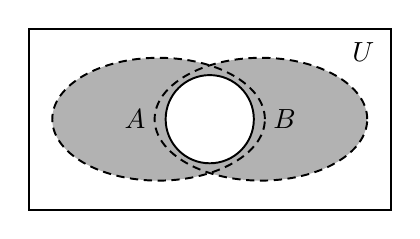
\begin{tikzpicture}[scale=1,line width=0.7pt]
\draw (0,0) rectangle (4.6,2.3);
\fill[black!30] (1.65,1.15) ellipse (1.35 and 0.78);
\fill[black!30] (2.95,1.15) ellipse (1.35 and 0.78);
\fill[white] (2.3,1.15) circle (0.56);
\draw[densely dashed] (1.65,1.15) ellipse (1.35 and 0.78);
\draw[densely dashed] (2.95,1.15) ellipse (1.35 and 0.78);
\draw (2.3,1.15) circle (0.56);
\node at (1.35,1.15) {$A$};
\node at (3.25,1.15) {$B$};
\node at (4.25,2.0) {$U$};
\end{tikzpicture}
\end{center}

\keepwithprev
A. $(-2,1)$\qquad B. $[-1,0]\cup[1,2)$\qquad C. $(-2,-1)\cup[0,1]$\qquad D. $[0,1]$

\ifanswer
\solbegin
\step{$A=\{x\mid-2<x<0\}$，$B=\{x\mid-1\leqslant x\leqslant1\}$，}
\step{所以 $A\cap B=\{x\mid-1\leqslant x<0\}$，$A\cup B=\{x\mid-2<x\leqslant1\}$，}
\step{则图中阴影部分表示的集合是 $(-2,-1)\cup[0,1]$，故选 $C$.}
\solend
\fi

\item 用反证法证明：“若 $x$、$y\in\R$ 且 $x+y>2$，则 $x$、$y$ 中至少有一个大于 $1$”时，应假设\mbox{（\quad）}% 原卷括号内已印“D”，试卷版按惯例留空

\keepwithprev
A. $x$、$y$ 中至少有一个小于 $1$\qquad B. $x$、$y$ 均小于 $1$

C. $x$、$y$ 中至少有一个小于等于 $1$\qquad D. $x$、$y$ 均小于等于 $1$

\ifanswer
\ans{$D$}
\fi

\item 若关于 $x$ 的不等式 $ax^2+bx+c>0$ 的解集是 $(-1,2)$，则不等式 $\dfrac{3ax-b}{x-3}>0$ 的解集是\mbox{（\quad）}

\keepwithprev
A. $\left(-\infty,-\dfrac13\right)\cup(3,+\infty)$\qquad B. $\left(-\dfrac13,3\right)$

C. $(-\infty,-3)\cup\left(\dfrac13,+\infty\right)$\qquad D. $\left(-3,\dfrac13\right)$

\ifanswer
\solbegin
\step{因为不等式 $ax^2+bx+c>0$ 的解集是 $(-1,2)$，}
\step{所以 $-1$、$2$ 是方程 $ax^2+bx+c=0$ 的两个根，且 $a<0$，}
\step{所以 $\begin{cases}-1+2=-\dfrac ba\\ -1\times2=\dfrac ca\end{cases}\Rightarrow\begin{cases}b=-a\\ c=-2a\end{cases}$，}
\step{所以 $\dfrac{3ax-b}{x-3}>0\Rightarrow\dfrac{3ax+a}{x-3}>0\Leftrightarrow a(3x+1)(x-3)>0$，}
\step{又 $a<0$，所以 $(3x+1)(x-3)<0$，解得 $-\dfrac13<x<3$，}
\step{所以不等式 $\dfrac{3ax-b}{x-3}>0$ 的解集为 $\left(-\dfrac13,3\right)$，故选 $B$.}
\solend
\fi

\end{enumerate}

\bigsec{三、解答题}

\begin{enumerate}
\setcounter{enumi}{16}

\item 解下列不等式组：

（1）$\begin{cases}\dfrac{5-x}{x+3}>0\\ 2x-\lvert x-1\rvert>2\end{cases}$；\qquad（2）$\begin{cases}-x^2+x+6\geqslant0\\ \dfrac{x-2}{x+1}\geqslant0\end{cases}$.

\ansspace*[12]

\ifanswer
\solbegin
\stepm{（1）}{不等式 $\dfrac{5-x}{x+3}>0$ 等价于 $(x-5)(x+3)<0$，所以 $-3<x<5$，}
\step{不等式 $2x-\lvert x-1\rvert>2$ 等价于 $2x-2>\lvert x-1\rvert$，}
\step{所以 $2-2x<x-1<2x-2$，故 $x>1$，}
\step{所以不等式组的解集为 $(1,5)$；}
\stepm{（2）}{不等式组 $\begin{cases}-x^2+x+6\geqslant0\\ \dfrac{x-2}{x+1}\geqslant0\end{cases}$ 可化为 $\begin{cases}x^2-x-6\leqslant0\\ (x-2)(x+1)\geqslant0\\ x+1\neq0\end{cases}$，}
\step{解得 $\begin{cases}-2\leqslant x\leqslant3\\ x\leqslant-1\ \text{或}\ x\geqslant2\\ x\neq-1\end{cases}$，即 $-2\leqslant x<-1$ 或 $2\leqslant x\leqslant3$，}
\step{所以不等式组的解集为 $\{x\mid-2\leqslant x<-1$ 或 $2\leqslant x\leqslant3\}$.}
\solend
\fi

\needvspace{3.2cm}
\item 已知 $A=\{x\mid x^2-2x-3\leqslant0\}$，$B=\{x\mid a-1\leqslant x\leqslant2a+1\}$，$a\in\R$.

（1）若 $A\cap B=B$，求实数 $a$ 的取值范围.

（2）若 $a>b>0$，比较 $\dfrac{a^2-b^2}{a^2+b^2}$ 与 $\dfrac{a-b}{a+b}$ 的大小.

\ansspace*[13]

\ifanswer
\solbegin
\stepm{（1）}{解不等式 $x^2-2x-3\leqslant0$，得 $-1\leqslant x\leqslant3$，}
\step{因为 $A\cap B=B$，所以 $B\subseteq A$，}
\step{当 $B=\varnothing$ 时，则 $a-1>2a+1$，解得 $a<-2$，}
\step{当 $B\neq\varnothing$ 时，要使得 $B\subseteq A$，则满足 $\begin{cases}a-1\leqslant2a+1\\ a-1\geqslant-1\\ 2a+1\leqslant3\end{cases}$，解得 $0\leqslant a\leqslant1$，}
\step{综上，实数 $a$ 的取值范围为 $(-\infty,-2)\cup[0,1]$.}
\stepm{（2）}{因为 $a>b>0$，所以 $a-b>0$，$a+b>0$，$ab>0$，}
\step{所以 $a^2-b^2=(a-b)(a+b)>0$，$a^2+b^2+2ab>a^2+b^2>0$，}
\step{$\dfrac{a^2-b^2}{a^2+b^2}>0$，$\dfrac{a-b}{a+b}>0$，}
\step{$\dfrac{\dfrac{a^2-b^2}{a^2+b^2}}{\dfrac{a-b}{a+b}}=\dfrac{(a-b)(a+b)}{a^2+b^2}\cdot\dfrac{a+b}{a-b}=\dfrac{a^2+b^2+2ab}{a^2+b^2}>1$，}
\step{所以 $\dfrac{a^2-b^2}{a^2+b^2}>\dfrac{a-b}{a+b}$.}
\solend
\fi

\item 汽车在行驶中，由于惯性作用，刹车后还要继续向前滑行一段距离才能停住，我们称这段距离为“刹车距离”. 刹车距离是分析事故的一个重要因素. 在一个限速 $40\mathrm{km}/\mathrm{h}$ 以内的弯道上，甲、乙两辆汽车相向而行，发现情况不对，同时刹车，但还是相碰了，事发后现场测得甲车的刹车距离略超过 $12\mathrm{m}$，乙车的刹车距离略超过 $10\mathrm{m}$，又知甲、乙两种车型的刹车距离 $s(\mathrm{m})$ 与车速 $x(\mathrm{km}/\mathrm{h})$ 之间有如下关系：$s_{\text{甲}}=0.1x+0.01x^2$，$s_{\text{乙}}=0.05x+0.005x^2$. 问：两车相撞的主要责任是谁？

\ansspace*[10]

\ifanswer
\solbegin
\step{由题意列出不等式组 $\begin{cases}0.1x+0.01x^2>12\\ 0.05x+0.005x^2>10\end{cases}$，解得 $\begin{cases}x<-40\ \text{或}\ x>30\\ x<-50\ \text{或}\ x>40\end{cases}$，}
\step{由于 $x>0$，从而可得 $x_{\text{甲}}>30\mathrm{km}/\mathrm{h}$，$x_{\text{乙}}>40\mathrm{km}/\mathrm{h}$.}
\step{经比较得乙车超过限速，应负主要责任.}
\solend
\fi

\item 已知关于 $x$ 的一元二次方程 $x^2+(2m-1)x+m^2-3=0$ 有实数根.

（1）若方程有两个负根，求实数 $m$ 的取值范围；

（2）当 $m=2$ 时，记方程的根为 $x_1$、$x_2$，求代数式 $\lvert x_1-x_2\rvert$ 的值.

\ansspace*[12]

\ifanswer
\solbegin
\stepm{（1）}{由方程有两个负根，得 $\begin{cases}\Delta=(2m-1)^2-4(m^2-3)\geqslant0\\ -(2m-1)<0\\ m^2-3>0\end{cases}$，}
\step{即 $\begin{cases}13-4m\geqslant0\\ 2m-1>0\\ (m-\sqrt3)(m+\sqrt3)>0\end{cases}$，解得 $\sqrt3<m\leqslant\dfrac{13}4$，}
\step{则实数 $m$ 的取值范围为 $\left\{m\left|\sqrt3<m\leqslant\dfrac{13}4\right.\right\}$.}
\stepm{（2）}{当 $m=2$ 时，方程为 $x^2+3x+1=0$，}
\step{此时 $\Delta=3^2-4=5>0$，且 $x_1+x_2=-3$，$x_1x_2=1$，}
\step{则 $\lvert x_1-x_2\rvert=\sqrt{(x_1+x_2)^2-4x_1x_2}=\sqrt{(-3)^2-4}=\sqrt5$.}
\solend
\fi

\item 已知不等式 $\lvert2x-a\rvert\leqslant b$ 的解集为 $A$，不等式 $mx^2-mx-1<0$ 的解集为 $B$.

（1）若 $a=1$，$b=2$，求 $A$.

（2）若 $A=[-1,3]$，求实数 $a$、$b$ 的取值；

（3）若 $B=\R$，求实数 $m$ 的取值范围.

\ansspace*[12]

\ifanswer
\solbegin
\stepm{（1）}{因为 $a=1$，$b=2$，所以不等式 $\lvert2x-a\rvert\leqslant b$ 等价于 $\lvert2x-1\rvert\leqslant2$，}
\step{所以 $-2\leqslant2x-1\leqslant2$，故 $-\dfrac12\leqslant x\leqslant\dfrac32$，所以 $A=\left[-\dfrac12,\dfrac32\right]$；}
\stepm{（2）}{当 $b>0$ 时，不等式 $\lvert2x-a\rvert\leqslant b$ 可化为 $-b\leqslant2x-a\leqslant b$，}
\step{所以 $\dfrac{a-b}2\leqslant x\leqslant\dfrac{a+b}2$，由 $A=[-1,3]$，得 $\dfrac{a-b}2=-1$，$\dfrac{a+b}2=3$；}
\step{当 $b=0$ 时，不等式 $\lvert2x-a\rvert\leqslant b$ 的解集为 $\left\{\dfrac a2\right\}$，不满足要求，}
\step{当 $b<0$ 时，不等式 $\lvert2x-a\rvert\leqslant b$ 的解集为 $\varnothing$，不满足要求，}
\step{所以 $a=2$，$b=4$；}
\stepm{（3）}{由已知不等式 $mx^2-mx-1<0$ 的解集为 $\R$，}
\step{得 $\begin{cases}m<0\\ m^2+4m<0\end{cases}$ 或 $m=0$，解得 $-4<m<0$ 或 $m=0$，}
\step{所以实数 $m$ 的取值范围为 $(-4,0]$.}
\solend
\fi

\end{enumerate}

\end{document}
"
%
% 原始材料：微信公众号“魔都数学加油站”文章，连载“27学年高一97”；
% 原文标题“27学年高一97——2026-2027年上海市浦东中学高一上10月月考”；
% 原文链接：https://mp.weixin.qq.com/s/2uW3LikOX3B07IWw7LkF_g。
% 正文为 8 张 PNG 页（`原图/高一97_浦东中学_10月月考/01..08.png`）：04、08 为
% 2560×3620，其余为 4762×6735，按页序读取。
%
% 篇幅与题号：原卷自第 3 题起编号（第 1、2 题不在原文内）。填空题 3—12（10 题）、
% 选择题 13—16（4 题）、解答题 17—21（5 题），共 19 题。
%
% 讲评版：第 15 题无【解析】、答案“D”直接印在题干括号内，本稿试卷版按惯例留空、
% 答案版提 \ans{}；其余 18 题印【解析】，其中第 13、14、16 题的答案在解析末句
% “故选 $B$／$C$／$B$”。
%
% 副标题：原卷未印副标题。本稿按内容标作“集合与常用逻辑用语、不等式”。
%
% 插图：第 14 题题干右侧有一幅韦恩图（全集 $U$ 的矩形内两个相交椭圆 $A$、$B$，
% 阴影为两椭圆的对称差）。原图该页为 2560×3620 的低分辨率页，直接裁切会糊，
% 故按原图布局用 TikZ 重绘（三版都出）。
%
% 与原卷的排版差异：
%   ① 原卷每题下直接印【答案】/【解析】，本稿按全稿惯例将答案与解析置于答案版；
%   ② 原卷未印副标题，本稿补出；填空横线统一排 \blankline[4.4em]；
%   ③ 原卷数集记号排斜体 $R$，本稿按全稿惯例改用 $\R$；
%   ④ 第 14 题的韦恩图原为行内右侧小图，本稿改为居中单列；
%   ⑤ 解答题按惯例加 \ansspace；选择题括号排 \mbox{（\quad）}。
%
% 行数核对：逐题数 \step/\stepm 条数，合计 85 条（Q3：2；Q4：2；Q5：2；Q6：2；
% Q7：2；Q8：4；Q9：4；Q10：5；Q11：10；Q12：3；Q13：4；Q14：3；Q15：0；
% Q16：6；Q17：7；Q18：10；Q19：3；Q20：6；Q21：10）。第 15 题无解析，
% 不计入 \step 账。原卷解析的换行按语意合并，未逐行强拆。
%
\documentclass[a4paper,11pt]{article}
\usepackage{common}

\begin{document}

\examtitlest[2]{2026--2027 年浦东中学高一上 10 月月考}{集合与常用逻辑用语、不等式}

\bigsec{一、填空题}

\begin{enumerate}
\setcounter{enumi}{2}

\item “$a(a-2)<0$”是“$\dfrac2a>1$”成立的\blankline[4.4em]条件（填充分必要性）.

\ifanswer
\solbegin
\step{“不等式 $a(a-2)<0\Rightarrow0<a<2$，不等式 $\dfrac2a>1\Rightarrow\dfrac{2-a}a>0\Rightarrow0<a<2$，}
\step{两不等式解集相等，所以“$a(a-2)<0$”是“$\dfrac2a>1$”成立的充要条件.}
\solend
\fi

\item 求不等式 $\lvert5-2x\rvert\leqslant3$ 的解集\blankline[4.4em].

\ifanswer
\solbegin
\step{$\lvert5-2x\rvert\leqslant3$ 等价于 $-3\leqslant5-2x\leqslant3$，解得 $1\leqslant x\leqslant4$，}
\step{所以不等式 $\lvert5-2x\rvert\leqslant3$ 的解集为 $\{x\mid1\leqslant x\leqslant4\}$.}
\solend
\fi

\item 求不等式组 $\begin{cases}3x^2+2x-1<0\\ \dfrac1x\geqslant0\end{cases}$ 的解集\blankline[4.4em].

\ifanswer
\solbegin
\step{不等式 $3x^2+2x-1=(3x-1)(x+1)<0$，解得 $-1<x<\dfrac13$，}
\step{由不等式 $\dfrac1x\geqslant0$ 解得 $x>0$，所以不等式组的解集为 $\left(0,\dfrac13\right)$.}
\solend
\fi

\item 满足 $\{1,3\}\subseteq A\subseteq\{0,1,3,5\}$ 的所有集合 $A$ 的全部元素之和为\blankline[4.4em].

\ifanswer
\solbegin
\step{符合条件的集合 $A$ 有以下几个，$A_1=\{0,1,3\}$，$A_2=\{1,3,5\}$，$A_3=\{0,1,3,5\}$，}
\step{所以所有集合 $A$ 的全部元素之和为 $0+1+3+1+3+5+0+1+3+5=22$.}
\solend
\fi

\item 已知集合 $A=\{(x,y)\mid y=-x+1\}$，$B=\{(x,y)\mid y=x^2-1\}$，则 $A\cap B=\blankline[4.4em]$.

\ifanswer
\solbegin
\step{联立 $\begin{cases}y=-x+1\\ y=x^2-1\end{cases}$，解得 $\begin{cases}x=1\\ y=0\end{cases}$ 或 $\begin{cases}x=-2\\ y=3\end{cases}$，}
\step{故 $A\cap B=\{(1,0),(-2,3)\}$.}
\solend
\fi

\item 若 $a$、$b$ 是方程 $x^2+2x-3=0$ 的两个实数根，则 $a^2-2b=\blankline[4.4em]$.

\ifanswer
\solbegin
\step{$a$、$b$ 是方程 $x^2+2x-3=0$ 的两个实数根，}
\step{所以 $a^2+2a-3=0$，故 $a^2=3-2a$，}
\step{由韦达定理得 $a+b=-2$，所以 $b=-2-a$，}
\step{所以 $a^2-2b=3-2a-2b=3-2a+4+2a=7$.}
\solend
\fi

\item 设 $a$、$b$ 为实数，若不等式 $x^2-ax-b<0$ 的解集为 $(2,8)$，则 $bx^2-ax-1>0$ 的解集为\blankline[4.4em].

\ifanswer
\solbegin
\step{因为不等式 $x^2-ax-b<0$ 的解集为 $(2,8)$，所以 $\begin{cases}2+8=a\\ 2\times8=-b\end{cases}$，}
\step{所以 $a=10$，$b=-16$，所以 $bx^2-ax-1>0$ 可化为 $-16x^2-10x-1>0$，}
\step{所以 $16x^2+10x+1<0$，}
\step{所以所求不等式的解集为 $\left(-\dfrac12,-\dfrac18\right)$.}
\solend
\fi

\item 若集合 $A=\{x\mid x^2+3x-4=0\}$，$B=\{x\mid ax-1=0\}$，若 $A\cap B=B$，则实数 $a$ 的取值组成的集合是\blankline[4.4em].

\ifanswer
\solbegin
\step{集合 $A=\{x\mid x^2+3x-4=0\}=\{-4,1\}$，$B=\{x\mid ax-1=0\}$，}
\step{因为 $A\cap B=B$，所以 $B\subseteq A$，}
\step{当 $a=0$ 时，$B=\varnothing$，$B\subseteq A$ 成立；}
\step{当 $a\neq0$ 时，$B=\left\{\dfrac1a\right\}$，由 $B\subseteq A$，得 $\dfrac1a=-4$ 或 $\dfrac1a=1$，解得 $a=-\dfrac14$ 或 $a=1$，}
\step{所以实数 $a$ 的值为 $-\dfrac14$ 或 $0$ 或 $1$，实数 $a$ 的取值组成的集合是 $\left\{-\dfrac14,0,1\right\}$.}
\solend
\fi

\item 关于 $x$ 的不等式 $ax^2+(1-2a^2)x-2a<0$ 的解集中恰有 $3$ 个正整数解，则 $a$ 的取值范围为\blankline[4.4em].

\ifanswer
\solbegin
\step{①当 $a=0$ 时，不等式化为 $x<0$，则解集中有无数个整数，不满足题意；}
\step{当 $a\neq0$ 时，不等式 $ax^2+(1-2a^2)x-2a<0$ 的解集中恰有 $3$ 个正整数解，}
\step{即为不等式 $(ax+1)(x-2a)<0$ 的解集中恰有 $3$ 个正整数解，}
\step{②当 $a<0$ 时，不等式 $(ax+1)(x-2a)<0$ 的解集中有无数个正整数，}
\step{不满足题意，}
\step{③当 $a>0$ 时，$-\dfrac1a<0,2a>0$，所以 $-\dfrac1a<2a$，}
\step{所以不等式的解集为 $\left\{x\left|-\dfrac1a<x<2a\right.\right\}$，}
\step{由解集得 $0$ 一定属于此集合，则由不等式的解集中恰有 $3$ 个正整数，}
\step{则这 $3$ 个正整数一定为 $1$，$2$，$3$，则 $3<2a\leqslant4$，解得 $\dfrac32<a\leqslant2$，}
\step{所以 $a$ 的取值范围是 $\left\{a\left|\dfrac32<a\leqslant2\right.\right\}$.}
\solend
\fi

\item 设 $x\in\R$，$[x]$ 表示不大于 $x$ 的最大整数，如 $[\pi]=3$，$[-1.2]=-2$，$\left[\dfrac12\right]=0$，则使 $[\lvert x-1\rvert]=3$ 成立的 $x$ 的取值范围\blankline[4.4em].

\ifanswer
\solbegin
\step{由题意 $[\lvert x-1\rvert]=3$，则 $3\leqslant\lvert x-1\rvert<4$，所以 $3\leqslant x-1<4$ 或 $-4\leqslant x-1<-3$，}
\step{解得 $4\leqslant x<5$ 或 $-3<x\leqslant-2$，}
\step{所以使 $[\lvert x-1\rvert]=3$ 成立的 $x$ 的取值范围是 $(-3,-2]\cup[4,5)$.}
\solend
\fi

\end{enumerate}

\bigsec{二、选择题}

\begin{enumerate}
\setcounter{enumi}{12}

\item 若 $a\in\R$，则“$a^2>a$”是“$a>1$”的\mbox{（\quad）}

\keepwithprev
A. 充分非必要条件\qquad B. 必要非充分条件

C. 充要条件\qquad D. 既非充分又非必要条件

\ifanswer
\solbegin
\step{已知 $a^2>a$，则 $a(a-1)>0$，即 $a<0$ 或 $a>1$，}
\step{由“$a<0$ 或 $a>1$”不能推出“$a>1$”；}
\step{由“$a>1$”可以推出“$a<0$ 或 $a>1$”，即“$a>1$”可以推出“$a^2>a$”；}
\step{所以“$a^2>a$”是“$a>1$”的必要非充分条件. 故选 $B$.}
\solend
\fi

\item 已知全集 $U=\R$，集合 $A=\{x\mid x(x+2)<0\}$，$B=\{x\mid\lvert x\rvert\leqslant1\}$，则图中阴影部分表示的集合是\mbox{（\quad）}

\begin{center}
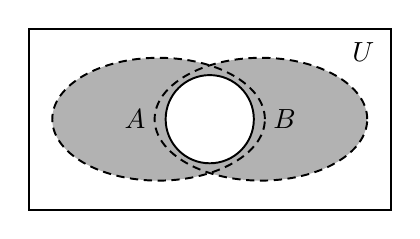
\begin{tikzpicture}[scale=1,line width=0.7pt]
\draw (0,0) rectangle (4.6,2.3);
\fill[black!30] (1.65,1.15) ellipse (1.35 and 0.78);
\fill[black!30] (2.95,1.15) ellipse (1.35 and 0.78);
\fill[white] (2.3,1.15) circle (0.56);
\draw[densely dashed] (1.65,1.15) ellipse (1.35 and 0.78);
\draw[densely dashed] (2.95,1.15) ellipse (1.35 and 0.78);
\draw (2.3,1.15) circle (0.56);
\node at (1.35,1.15) {$A$};
\node at (3.25,1.15) {$B$};
\node at (4.25,2.0) {$U$};
\end{tikzpicture}
\end{center}

\keepwithprev
A. $(-2,1)$\qquad B. $[-1,0]\cup[1,2)$\qquad C. $(-2,-1)\cup[0,1]$\qquad D. $[0,1]$

\ifanswer
\solbegin
\step{$A=\{x\mid-2<x<0\}$，$B=\{x\mid-1\leqslant x\leqslant1\}$，}
\step{所以 $A\cap B=\{x\mid-1\leqslant x<0\}$，$A\cup B=\{x\mid-2<x\leqslant1\}$，}
\step{则图中阴影部分表示的集合是 $(-2,-1)\cup[0,1]$，故选 $C$.}
\solend
\fi

\item 用反证法证明：“若 $x$、$y\in\R$ 且 $x+y>2$，则 $x$、$y$ 中至少有一个大于 $1$”时，应假设\mbox{（\quad）}% 原卷括号内已印“D”，试卷版按惯例留空

\keepwithprev
A. $x$、$y$ 中至少有一个小于 $1$\qquad B. $x$、$y$ 均小于 $1$

C. $x$、$y$ 中至少有一个小于等于 $1$\qquad D. $x$、$y$ 均小于等于 $1$

\ifanswer
\ans{$D$}
\fi

\item 若关于 $x$ 的不等式 $ax^2+bx+c>0$ 的解集是 $(-1,2)$，则不等式 $\dfrac{3ax-b}{x-3}>0$ 的解集是\mbox{（\quad）}

\keepwithprev
A. $\left(-\infty,-\dfrac13\right)\cup(3,+\infty)$\qquad B. $\left(-\dfrac13,3\right)$

C. $(-\infty,-3)\cup\left(\dfrac13,+\infty\right)$\qquad D. $\left(-3,\dfrac13\right)$

\ifanswer
\solbegin
\step{因为不等式 $ax^2+bx+c>0$ 的解集是 $(-1,2)$，}
\step{所以 $-1$、$2$ 是方程 $ax^2+bx+c=0$ 的两个根，且 $a<0$，}
\step{所以 $\begin{cases}-1+2=-\dfrac ba\\ -1\times2=\dfrac ca\end{cases}\Rightarrow\begin{cases}b=-a\\ c=-2a\end{cases}$，}
\step{所以 $\dfrac{3ax-b}{x-3}>0\Rightarrow\dfrac{3ax+a}{x-3}>0\Leftrightarrow a(3x+1)(x-3)>0$，}
\step{又 $a<0$，所以 $(3x+1)(x-3)<0$，解得 $-\dfrac13<x<3$，}
\step{所以不等式 $\dfrac{3ax-b}{x-3}>0$ 的解集为 $\left(-\dfrac13,3\right)$，故选 $B$.}
\solend
\fi

\end{enumerate}

\bigsec{三、解答题}

\begin{enumerate}
\setcounter{enumi}{16}

\item 解下列不等式组：

（1）$\begin{cases}\dfrac{5-x}{x+3}>0\\ 2x-\lvert x-1\rvert>2\end{cases}$；\qquad（2）$\begin{cases}-x^2+x+6\geqslant0\\ \dfrac{x-2}{x+1}\geqslant0\end{cases}$.

\ansspace*[12]

\ifanswer
\solbegin
\stepm{（1）}{不等式 $\dfrac{5-x}{x+3}>0$ 等价于 $(x-5)(x+3)<0$，所以 $-3<x<5$，}
\step{不等式 $2x-\lvert x-1\rvert>2$ 等价于 $2x-2>\lvert x-1\rvert$，}
\step{所以 $2-2x<x-1<2x-2$，故 $x>1$，}
\step{所以不等式组的解集为 $(1,5)$；}
\stepm{（2）}{不等式组 $\begin{cases}-x^2+x+6\geqslant0\\ \dfrac{x-2}{x+1}\geqslant0\end{cases}$ 可化为 $\begin{cases}x^2-x-6\leqslant0\\ (x-2)(x+1)\geqslant0\\ x+1\neq0\end{cases}$，}
\step{解得 $\begin{cases}-2\leqslant x\leqslant3\\ x\leqslant-1\ \text{或}\ x\geqslant2\\ x\neq-1\end{cases}$，即 $-2\leqslant x<-1$ 或 $2\leqslant x\leqslant3$，}
\step{所以不等式组的解集为 $\{x\mid-2\leqslant x<-1$ 或 $2\leqslant x\leqslant3\}$.}
\solend
\fi

\needvspace{3.2cm}
\item 已知 $A=\{x\mid x^2-2x-3\leqslant0\}$，$B=\{x\mid a-1\leqslant x\leqslant2a+1\}$，$a\in\R$.

（1）若 $A\cap B=B$，求实数 $a$ 的取值范围.

（2）若 $a>b>0$，比较 $\dfrac{a^2-b^2}{a^2+b^2}$ 与 $\dfrac{a-b}{a+b}$ 的大小.

\ansspace*[13]

\ifanswer
\solbegin
\stepm{（1）}{解不等式 $x^2-2x-3\leqslant0$，得 $-1\leqslant x\leqslant3$，}
\step{因为 $A\cap B=B$，所以 $B\subseteq A$，}
\step{当 $B=\varnothing$ 时，则 $a-1>2a+1$，解得 $a<-2$，}
\step{当 $B\neq\varnothing$ 时，要使得 $B\subseteq A$，则满足 $\begin{cases}a-1\leqslant2a+1\\ a-1\geqslant-1\\ 2a+1\leqslant3\end{cases}$，解得 $0\leqslant a\leqslant1$，}
\step{综上，实数 $a$ 的取值范围为 $(-\infty,-2)\cup[0,1]$.}
\stepm{（2）}{因为 $a>b>0$，所以 $a-b>0$，$a+b>0$，$ab>0$，}
\step{所以 $a^2-b^2=(a-b)(a+b)>0$，$a^2+b^2+2ab>a^2+b^2>0$，}
\step{$\dfrac{a^2-b^2}{a^2+b^2}>0$，$\dfrac{a-b}{a+b}>0$，}
\step{$\dfrac{\dfrac{a^2-b^2}{a^2+b^2}}{\dfrac{a-b}{a+b}}=\dfrac{(a-b)(a+b)}{a^2+b^2}\cdot\dfrac{a+b}{a-b}=\dfrac{a^2+b^2+2ab}{a^2+b^2}>1$，}
\step{所以 $\dfrac{a^2-b^2}{a^2+b^2}>\dfrac{a-b}{a+b}$.}
\solend
\fi

\item 汽车在行驶中，由于惯性作用，刹车后还要继续向前滑行一段距离才能停住，我们称这段距离为“刹车距离”. 刹车距离是分析事故的一个重要因素. 在一个限速 $40\mathrm{km}/\mathrm{h}$ 以内的弯道上，甲、乙两辆汽车相向而行，发现情况不对，同时刹车，但还是相碰了，事发后现场测得甲车的刹车距离略超过 $12\mathrm{m}$，乙车的刹车距离略超过 $10\mathrm{m}$，又知甲、乙两种车型的刹车距离 $s(\mathrm{m})$ 与车速 $x(\mathrm{km}/\mathrm{h})$ 之间有如下关系：$s_{\text{甲}}=0.1x+0.01x^2$，$s_{\text{乙}}=0.05x+0.005x^2$. 问：两车相撞的主要责任是谁？

\ansspace*[10]

\ifanswer
\solbegin
\step{由题意列出不等式组 $\begin{cases}0.1x+0.01x^2>12\\ 0.05x+0.005x^2>10\end{cases}$，解得 $\begin{cases}x<-40\ \text{或}\ x>30\\ x<-50\ \text{或}\ x>40\end{cases}$，}
\step{由于 $x>0$，从而可得 $x_{\text{甲}}>30\mathrm{km}/\mathrm{h}$，$x_{\text{乙}}>40\mathrm{km}/\mathrm{h}$.}
\step{经比较得乙车超过限速，应负主要责任.}
\solend
\fi

\item 已知关于 $x$ 的一元二次方程 $x^2+(2m-1)x+m^2-3=0$ 有实数根.

（1）若方程有两个负根，求实数 $m$ 的取值范围；

（2）当 $m=2$ 时，记方程的根为 $x_1$、$x_2$，求代数式 $\lvert x_1-x_2\rvert$ 的值.

\ansspace*[12]

\ifanswer
\solbegin
\stepm{（1）}{由方程有两个负根，得 $\begin{cases}\Delta=(2m-1)^2-4(m^2-3)\geqslant0\\ -(2m-1)<0\\ m^2-3>0\end{cases}$，}
\step{即 $\begin{cases}13-4m\geqslant0\\ 2m-1>0\\ (m-\sqrt3)(m+\sqrt3)>0\end{cases}$，解得 $\sqrt3<m\leqslant\dfrac{13}4$，}
\step{则实数 $m$ 的取值范围为 $\left\{m\left|\sqrt3<m\leqslant\dfrac{13}4\right.\right\}$.}
\stepm{（2）}{当 $m=2$ 时，方程为 $x^2+3x+1=0$，}
\step{此时 $\Delta=3^2-4=5>0$，且 $x_1+x_2=-3$，$x_1x_2=1$，}
\step{则 $\lvert x_1-x_2\rvert=\sqrt{(x_1+x_2)^2-4x_1x_2}=\sqrt{(-3)^2-4}=\sqrt5$.}
\solend
\fi

\item 已知不等式 $\lvert2x-a\rvert\leqslant b$ 的解集为 $A$，不等式 $mx^2-mx-1<0$ 的解集为 $B$.

（1）若 $a=1$，$b=2$，求 $A$.

（2）若 $A=[-1,3]$，求实数 $a$、$b$ 的取值；

（3）若 $B=\R$，求实数 $m$ 的取值范围.

\ansspace*[12]

\ifanswer
\solbegin
\stepm{（1）}{因为 $a=1$，$b=2$，所以不等式 $\lvert2x-a\rvert\leqslant b$ 等价于 $\lvert2x-1\rvert\leqslant2$，}
\step{所以 $-2\leqslant2x-1\leqslant2$，故 $-\dfrac12\leqslant x\leqslant\dfrac32$，所以 $A=\left[-\dfrac12,\dfrac32\right]$；}
\stepm{（2）}{当 $b>0$ 时，不等式 $\lvert2x-a\rvert\leqslant b$ 可化为 $-b\leqslant2x-a\leqslant b$，}
\step{所以 $\dfrac{a-b}2\leqslant x\leqslant\dfrac{a+b}2$，由 $A=[-1,3]$，得 $\dfrac{a-b}2=-1$，$\dfrac{a+b}2=3$；}
\step{当 $b=0$ 时，不等式 $\lvert2x-a\rvert\leqslant b$ 的解集为 $\left\{\dfrac a2\right\}$，不满足要求，}
\step{当 $b<0$ 时，不等式 $\lvert2x-a\rvert\leqslant b$ 的解集为 $\varnothing$，不满足要求，}
\step{所以 $a=2$，$b=4$；}
\stepm{（3）}{由已知不等式 $mx^2-mx-1<0$ 的解集为 $\R$，}
\step{得 $\begin{cases}m<0\\ m^2+4m<0\end{cases}$ 或 $m=0$，解得 $-4<m<0$ 或 $m=0$，}
\step{所以实数 $m$ 的取值范围为 $(-4,0]$.}
\solend
\fi

\end{enumerate}

\end{document}
